%!Tex Program=xelatex
\documentclass[12pt,a4paper,twoside,openany]{book}

%%%%%%%%%%导入相关宏包%%%%%%%%%%%%%%%%%%%%%%

\usepackage{CJKutf8,CJKnumb}
\usepackage{amsmath, amssymb,amsthm,amscd}
\usepackage{gensymb}
\usepackage{titlesec}
\usepackage{titletoc}
\usepackage{fancyhdr}
\usepackage[paperwidth=185mm,paperheight=260mm,text={148mm,210mm},
			left=21mm,vmarginratio=1:1]{geometry}
\usepackage{xcolor}
\usepackage{listings}
\usepackage{enumitem}
\usepackage[labelfont=bf,labelsep=quad]{caption}
\usepackage{multirow}
\usepackage{floatrow}
\usepackage{subfig}
\newif\ifpdf
\ifx\pdfoutput\undefined
   \pdffalse
\else
   \pdfoutput=1
   \pdftrue
\fi
\ifpdf
   \usepackage[pdftex]{graphicx}
   \usepackage[pdftex,unicode=true,colorlinks,linkcolor=red,anchorcolor=blue,citecolor=green]{hyperref}
\else
   \usepackage{graphicx}
   \usepackage[unicode={true},colorlinks,linkcolor=red,anchorcolor=blue,citecolor=green]{hyperref}
\fi
\usepackage{lscape}
\usepackage{tikz}
\usepackage{indentfirst}
\usetikzlibrary{arrows,calc,through}
\usetikzlibrary{intersections}

\setlength{\parindent}{2em}
\endinput

\makeindex%生成建立索引

\begin{document}
%%%%%%%%%% 定理类环境的定义 %%%%%%%%%% 
%% 必须在导入中文环境之后 
\newtheorem{example}{例}             % 整体编号 
\newtheorem{algorithm}{算法} 
\newtheorem{theorem}{定理}[section]  % 按 section 编号 
\newtheorem{definition}{定义} 
\newtheorem{axiom}{公理} 
\newtheorem{property}{性质} 
\newtheorem{proposition}{命题} 
\newtheorem{lemma}{引理} 
\newtheorem{corollary}{推论} 
\newtheorem{remark}{注解} 
\newtheorem{condition}{条件} 
\newtheorem{conclusion}{结论} 
\newtheorem{assumption}{假设} 
 
%%%%%%%%%% 一些重定义 %%%%%%%%%% 

%% 必须在导入中文环境之后 
\renewcommand{\contentsname}{目\quad 录}% 将 Contents 改为目录 
%\renewcommand{\abstractname}{摘\ \ 要} % 将 Abstract 改为摘要 
\renewcommand{\bibname}{参考文献}      % 将 References 改为参考文献 
\renewcommand{\indexname}{索\quad 引} %将Idex 改为索引
\renewcommand{\figurename}{图} 
\renewcommand{\tablename}{表} 
\renewcommand{\appendixname}{附\quad 录} 
\renewcommand{\proofname}{\hei 证明} 
\renewcommand{\algorithm}{\hei 算法} 
 
%%%%%%%%%% 重定义字号命令 %%%%%%%%%% 

\newcommand{\yihao}{\fontsize{26pt}{36pt}\selectfont}%一号, 1.4 倍行距 
\newcommand{\erhao}{\fontsize{22pt}{28pt}\selectfont}%二号, 1.25 倍行距 
\newcommand{\xiaoer}{\fontsize{18pt}{18pt}\selectfont}%小二, 单倍行距 
\newcommand{\sanhao}{\fontsize{16pt}{24pt}\selectfont}%三号, 1.5 倍行距
\newcommand{\xiaosan}{\fontsize{15pt}{22pt}\selectfont}%小三, 1.5 倍行距 
\newcommand{\sihao}{\fontsize{14pt}{21pt}\selectfont}%四号, 1.5 倍行距 
\newcommand{\bansi}{\fontsize{13pt}{19.5pt}\selectfont}%半四, 1.5 倍行距 
\newcommand{\xiaosi}{\fontsize{12pt}{18pt}\selectfont}% 小四, 1.5 倍行距 
\newcommand{\dawu}{\fontsize{11pt}{11pt}\selectfont} % 大五, 单倍行距 
\newcommand{\wuhao}{\fontsize{10.5pt}{10.5pt}\selectfont}%五号, 单倍行距

%%%%%%%%%%%%%重定义章节的格式%%%%%%%%%%%%%%%%%%%

\titlecontents{chapter}[1em]{\vspace{.5\baselineskip}\bfseries}
{第\thecontentslabel 章\quad}{}
{\hspace{.5em}\titlerule*[10pt]{$\cdot$}\contentspage}
\renewcommand{\chaptername}{第\,\thechapter \,章}
\titleformat{\chapter}[hang]{\centering\huge\bfseries}{\chaptername}{1em}{}
\titlespacing{\chapter}{0pt}{*0}{*4}
\pagestyle{fancy}
\fancyhf{}
\renewcommand{\chaptermark}[1]{\markboth{第\,\thechapter\,章\ #1}{}}
\renewcommand{\sectionmark}[1]{\markright{\thesection\ #1}{}}
%%%%%%%%%%%%定义页眉而脚%%%%%%%%%%%%%%%%%%%%%%%%%%%%%%%%%

\fancyhead[ER]{\leftmark}
\fancyhead[OL]{\rightmark}
\fancyhead[EL,OR]{$\cdot$\ \thepage\ $\cdot$}
\renewcommand{\headrulewidth}{0.4pt}

%%%%%%%%%%%%%设置列表格式%%%%%%%%%%%%%%%%

\setenumerate[1]{itemsep=0pt,partopsep=0pt,parsep=\parskip,topsep=5pt}

\setitemize[1]{itemsep=0pt,partopsep=0pt,parsep=\parskip,topsep=5pt}

\setdescription{itemsep=0pt,partopsep=0pt,parsep=\parskip,topsep=5pt}

%%%%%%%%%%%定义过程列表%%%%%%%%%%%%%%%%%

\newcommand{\gorectangle}[1]{
\tikz\node[text=white,font=\sffamily\bfseries,inner sep=0.5mm,draw,rounded corners,fill=black]{\small #1};}
\newcounter{procedurecounter}
\newenvironment{procedure}{
\begin{list}{\gorectangle{Step\,\arabic{procedurecounter}}}{
\setlength{\parsep}{\parskip}
\setlength{\itemsep}{0ex plus 0.1ex}
\setlength{\labelwidth}{4em}
\setlength{\labelsep}{0.2em}
\setlength{\leftmargin}{6.2em}
\usecounter{procedurecounter}
\setcounter{procedurecounter}{0}}}
{\end{list}}

\newcounter{yaodiancounter}
\tikzstyle{mybox} = [draw=black, fill=gray!20, very thick,
    rectangle, rounded corners, inner sep=10pt, inner ysep=20pt]
\tikzstyle{fancytitle} =[fill=gray, text=white]
\newcommand{\yaodian}[1]{
\addtocounter{yaodiancounter}{1}
\begin{tikzpicture}
\node [mybox] (box){%
    \begin{minipage}{0.75\textwidth}
       \lishu{#1}
    \end{minipage}
};
\node[fancytitle, right=10pt] at (box.north west) {\hei{要点\arabic{yaodiancounter}}};
\end{tikzpicture}
}
%源代码格式设置
\lstdefinelanguage{autocad}{
morekeywords={line, circle,xline,view,subtract,cylinder,vscurrent,union,chamferedge,save,saveas},
sensitive=false,
}
\lstloadlanguages{autocad}                  % 所要粘贴代码的编程语言 
\lstset{language=autocad,tabsize=4, keepspaces=true, 
    xleftmargin=2em,xrightmargin=2em, aboveskip=1em, 
    backgroundcolor=\color{lightgray},    % 定义背景颜色 
    frame=none,                      % 表示不要边框 
    keywordstyle=\color{blue}\bfseries,     breakindent=22pt,stepnumber=1,numberstyle=\tiny, 
    basicstyle=\footnotesize, 
    showspaces=false, 
    flexiblecolumns=true, 
    breaklines=true, breakautoindent=true,breakindent=4em, 
    escapeinside={/*@}{@*/} 
} 
\endinput
\title{\hei{\yihao{ 工程制图与CAD讲义}}}
\author{\sanhao{金波}}
\date{\today}
\maketitle
%\CJKtilde
\frontmatter
\chapter*{前言}
\section*{本书结构}
\section*{目标读者}
\section*{命令提示说明}
书中用到的相关命令及提示都会以代码的形式贴出。对于第一次出现的命令则会根据命令的提示进行逐步讲解,其形式如下:
\begin{lstlisting}
命令:CYLINDER
\end{lstlisting}

命令提示指定圆柱体的底面中心点或者绘图选项。
\begin{lstlisting}
指定底面的中心点或 [三点(3P)/两点(2P)/切点、切点、半径(T)/椭圆(E)]:
\end{lstlisting}

接下来,根据命令提示输入底面的半径
\begin{lstlisting}
指定底面半径或 [直径(D)]: 7
\end{lstlisting}

最后,根据命令提示指定圆柱体的高度,并按回车或空格键结束命令。
\begin{lstlisting}
指定高度或 [两点(2P)/轴端点(A)]: 28
\end{lstlisting}

对于已经使用过的命令,则直接贴整个命令提示,其形式如下:

\begin{lstlisting}
命令: CYLINDER
指定底面的中心点或 [三点(3P)/两点(2P)/切点、切点、半径(T)/椭圆(E)]:
指定底面半径或 [直径(D)]: 8
指定高度或 [两点(2P)/轴端点(A)]: 2
\end{lstlisting}
\section*{关于勘误}
由于编者的时间和水平比较有限,书中难免会出现一些纰漏和错误。如果读者在阅读过程中发现任何错误,请及时与本人联系,提出修改意见和建议。本人会在本书后续的版本中加以改正。本人专门为本书设立的电子邮箱是:kingbo2001@gmail.com。本人欢迎并希望和大家一起学习和讨论AutoCAD的三维建模功能,促进大家的共同进步。
\section*{致谢}
\endinput
\tableofcontents
\mainmatter
\graphicspath{{pdf/}{png/}}
\part{小轮组三维建模}
作为本书的第一部分,我们将构建小轮组组成零件的三维模型和小轮组装配三维模型。通过完成小轮组三维建模任务,让读者对应用AutoCAD进行三维建模的特点具有初步的认识和了解,掌握和理解以下几个方面的内容:
\begin{itemize}
\item 零件图和三维模型之间的对应关系
\item AutoCAD基本的三维建模命令
\item 三视图规律
\item 相关的国家制图标准
\item AutoCAD生成基本视图的方法
\end{itemize} 
%%%%%%%%%%%%%第一章%%%%%%%%%%%%%%%%%%%%%%%
\chapter{套筒}
\begin{figure}[htbp]
\centering
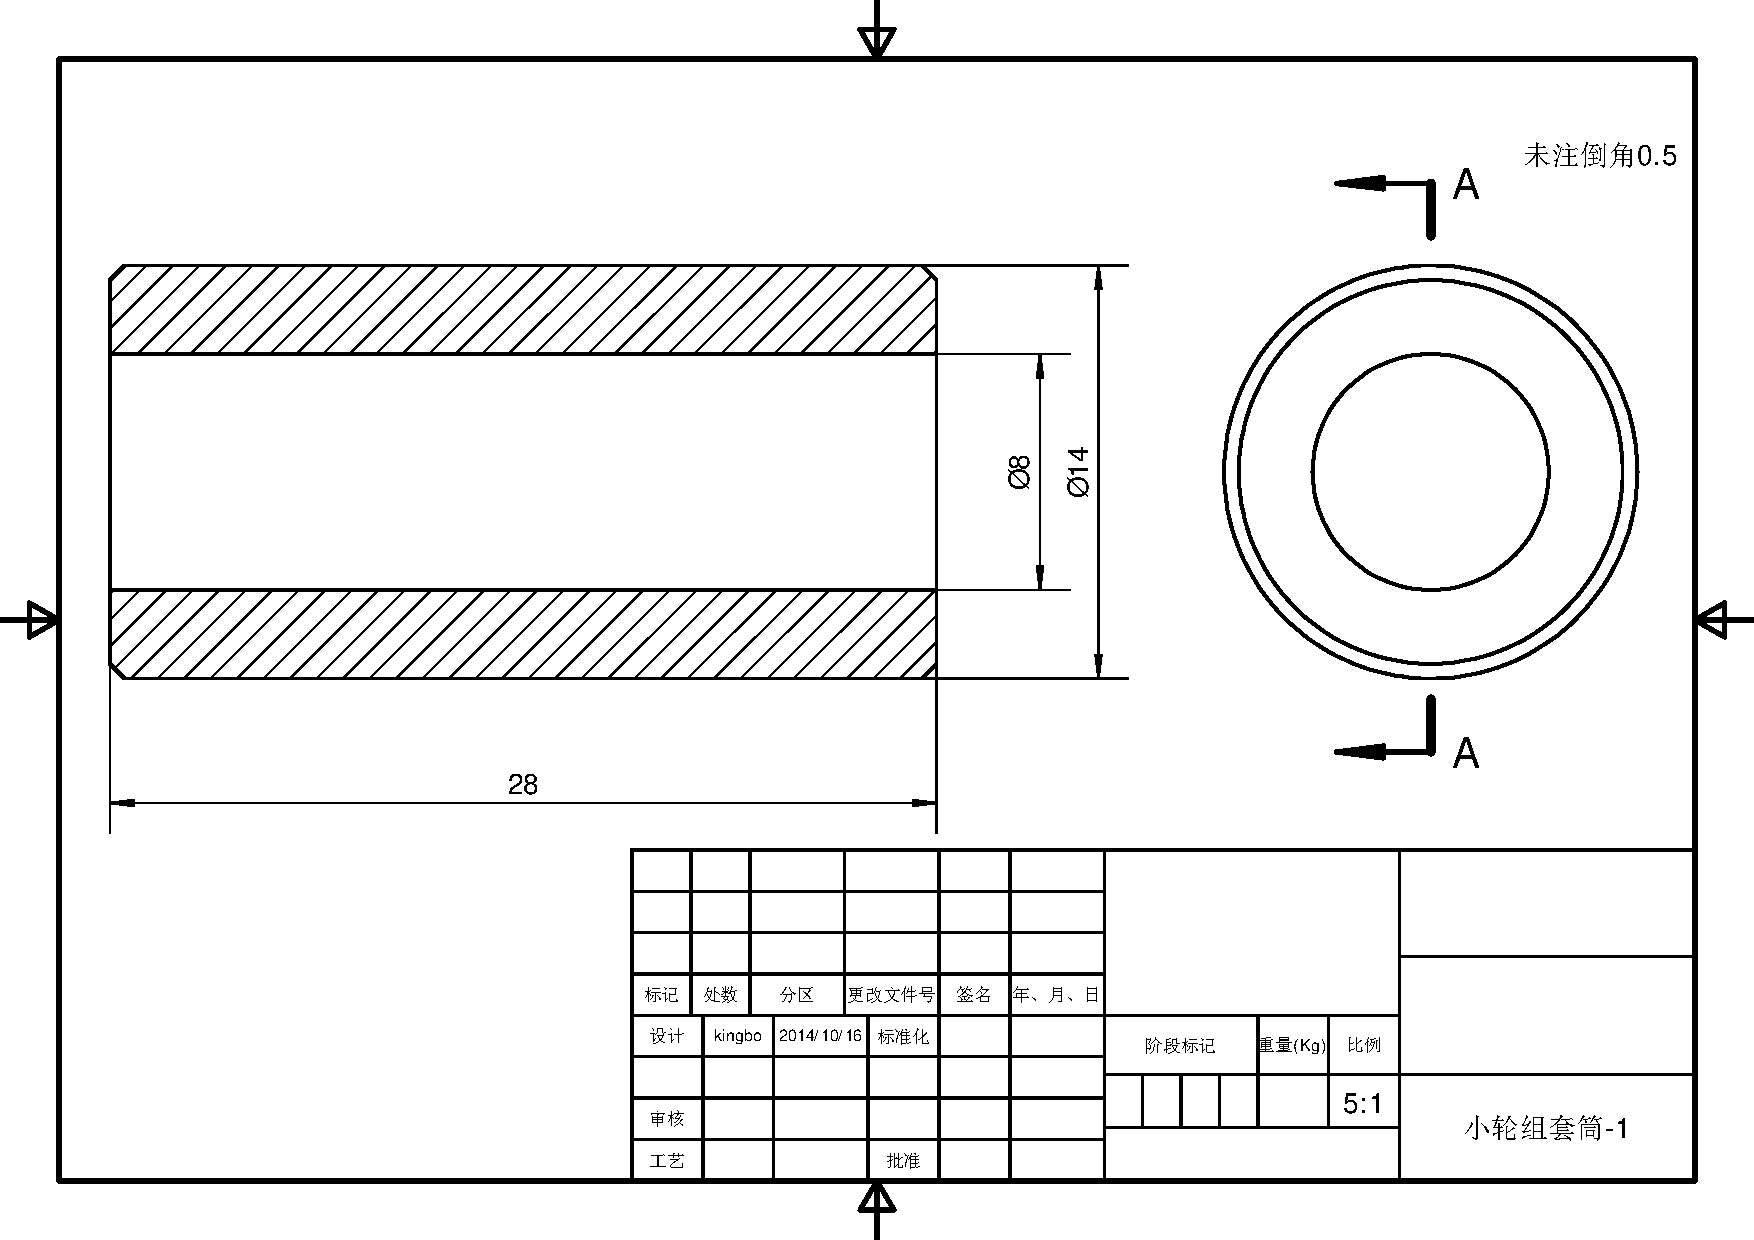
\includegraphics[scale=0.5]{xiaoluntaotong.pdf}
\end{figure}
\section{初识零件图}
在构建图\ref{fig:xiaoluntaotong}所示零件之前,让我们先来了解一些相关的制图知识。类似于图\ref{fig:xiaoluntaotong}所示的图纸被称为零件图。所谓零件图是用于表达零件的图样,它广泛运用于工程技术设计、施工或产品制造,它是制造、加工、测量、检验的依据,是工程界的共同技术语言,是表达和交流技术思想的必备工具,是工程技术部门的一项重要技术文件。掌握零件图的阅读和绘制不仅是构建零件三维模型的基础,也是从事工程设计和技术的工程技术人员所必须具备的基本能力。一张完整的零件图应包括以下几个组成部分:
\begin{itemize}
\item 一组视图
根据国家制图标准规定的视图、剖视、剖面及其他画法绘制的用于表达零件内外形状的图形。
\item 完整的尺寸
用于确定零件各部分形状大小和位置的全部尺寸。它是按照国家标准GT/T4458.4-1984的要求进行标注的。
\item 技术要求
用于规定零件在制造和检验时应达到的一些要求。通常用规定的符号标注于图纸中或在图纸上指定位置用文字统一标出。
\item 标题栏
用于说明零件的名称、材料、数量等信息。它是按照国家标准GB/T10609.1-1989的规定绘制的。
\end{itemize}
\begin{figure}[htbp]
\centering
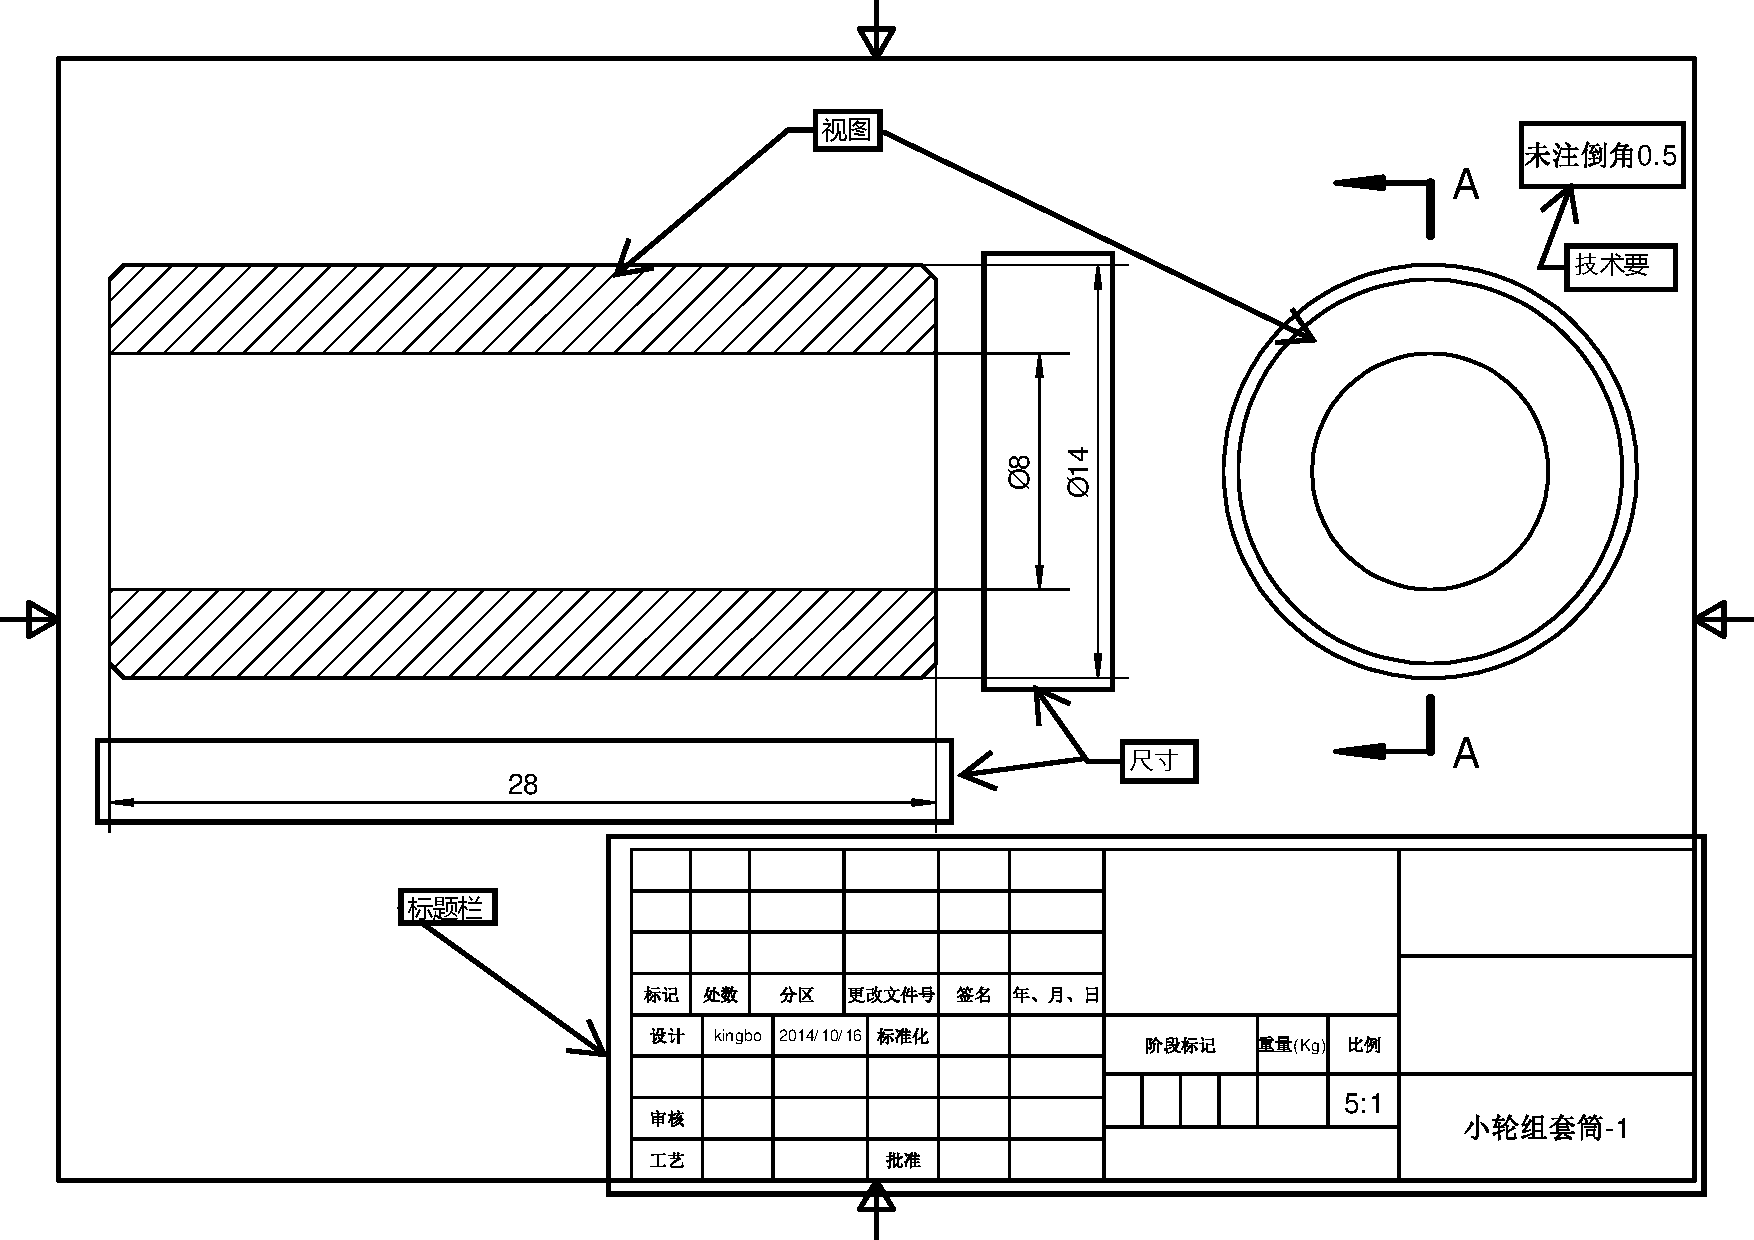
\includegraphics[scale=0.45]{xiaoluntaotong2.pdf}
\caption{零件图组成部分}\label{fig:xiaoluntaotong2}
\end{figure}
图\ref{fig:xiaoluntaotong2}对图\ref{fig:xiaoluntaotong}所示零件图的各个组成部分进行了标注。
\section{圆柱体视图}
图\ref{fig:xiaoluntaotong}所示零件图中的视图既然是用于表达零件的内外形状的,那么它的立体形状是怎样的呢,如保用AutoCAD构建出它的三维模型呢?要解决这个问题,我们先将图\ref{fig:xiaoluntaotong}所示零件图进行简化,忽略其内部及细微的局部,只研究其中$\phi 14$所对应的部分,简化后的结果如图\ref{fig:yuanzhuti}所示。
\begin{figure}[htbp]
\centering
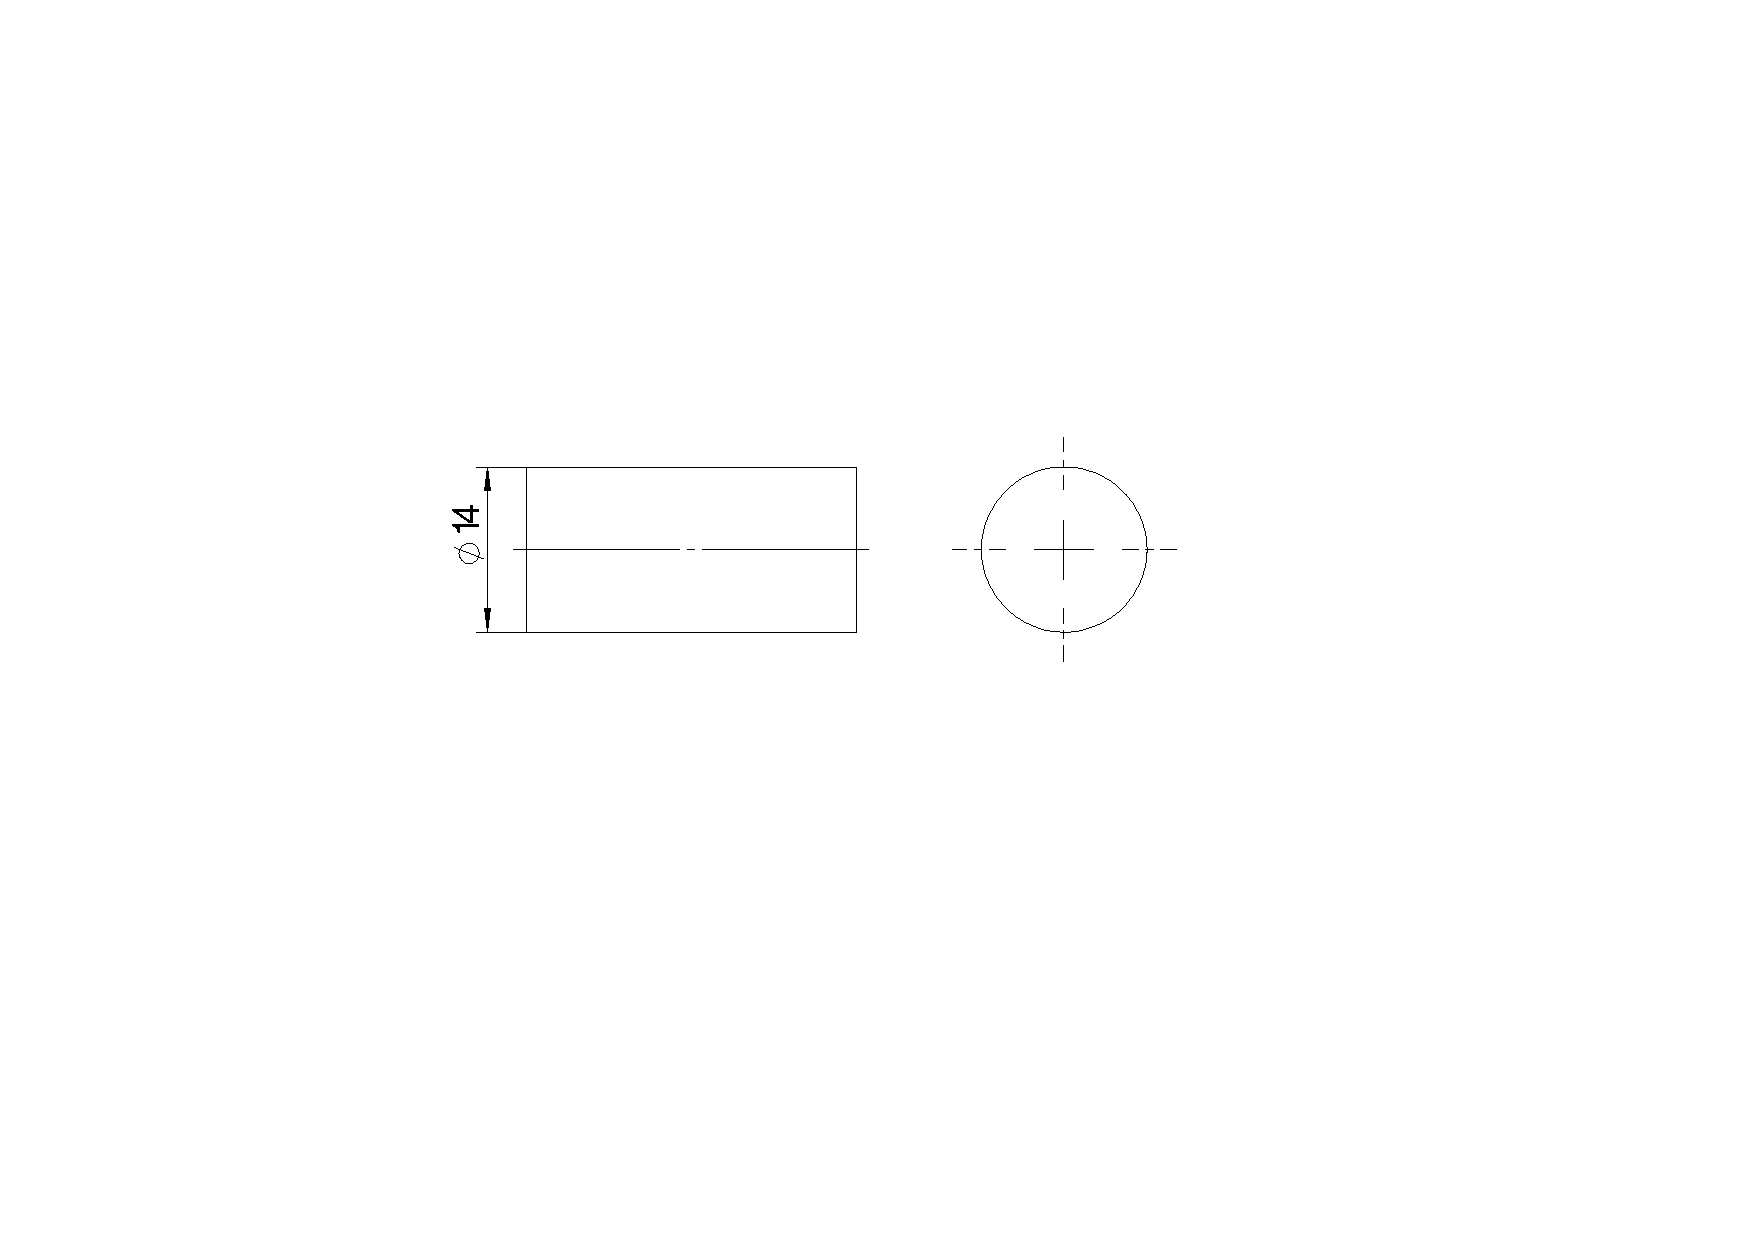
\includegraphics[scale=0.55]{yuanzhuti.pdf}
\caption{套筒外圆柱视图}\label{fig:yuanzhuti}
\end{figure}

那么图\ref{fig:yuanzhuti}所表达的又是什么物体呢?要回答这个问题,我们先将一个圆柱体放置于图\ref{fig:sanweizuobiao}所示的三个相互垂直的三面投影之中,然后从三个方向将圆柱体投影到投影面上,即可得到圆柱体的三面投影,如图\ref{fig:yuanzhutouyin}所示。从圆柱体的三面投影可以看出其中两投影的大小和形状是一样的,均为矩形,仅有一个投影为圆。
\begin{figure}[htbp]
\centering
\subfloat[三维投影面]{\label{fig:sanweizuobiao}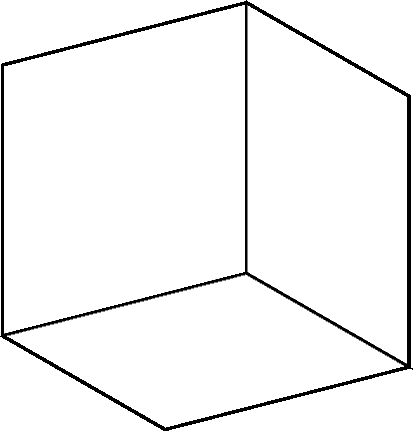
\includegraphics[scale=0.4]{sanweizuobiao.png}}\hspace{30pt}
\subfloat[圆柱体三面投影]{\label{fig:yuanzhutouyin}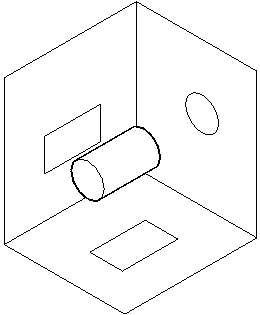
\includegraphics[scale=0.3]{yuanzhutouyin.png}}
\end{figure}

由此可以看出图\ref{fig:yuanzhuti}所示的视图表达的是一个直径为$\phi 14$,长为28的圆柱体,其中符号$\phi$用于表示后面所标注的尺寸是直径。

\endinput
\endinput
\section{初识零件图}
在构建图\ref{fig:xiaoluntaotong}所示零件之前,让我们先来了解一些相关的制图知识。类似于图\ref{fig:xiaoluntaotong}所示的图纸被称为零件图。所谓零件图是用于表达零件的图样,它广泛运用于工程技术设计、施工或产品制造,它是制造、加工、测量、检验的依据,是工程界的共同技术语言,是表达和交流技术思想的必备工具,是工程技术部门的一项重要技术文件。掌握零件图的阅读和绘制不仅是构建零件三维模型的基础,也是从事工程设计和技术的工程技术人员所必须具备的基本能力。一张完整的零件图应包括以下几个组成部分:
\begin{itemize}
\item 一组视图
根据国家制图标准规定的视图、剖视、剖面及其他画法绘制的用于表达零件内外形状的图形。
\item 完整的尺寸
用于确定零件各部分形状大小和位置的全部尺寸。它是按照国家标准GT/T4458.4-1984的要求进行标注的。
\item 技术要求
用于规定零件在制造和检验时应达到的一些要求。通常用规定的符号标注于图纸中或在图纸上指定位置用文字统一标出。
\item 标题栏
用于说明零件的名称、材料、数量等信息。它是按照国家标准GB/T10609.1-1989的规定绘制的。
\end{itemize}
\begin{figure}[htbp]
\centering
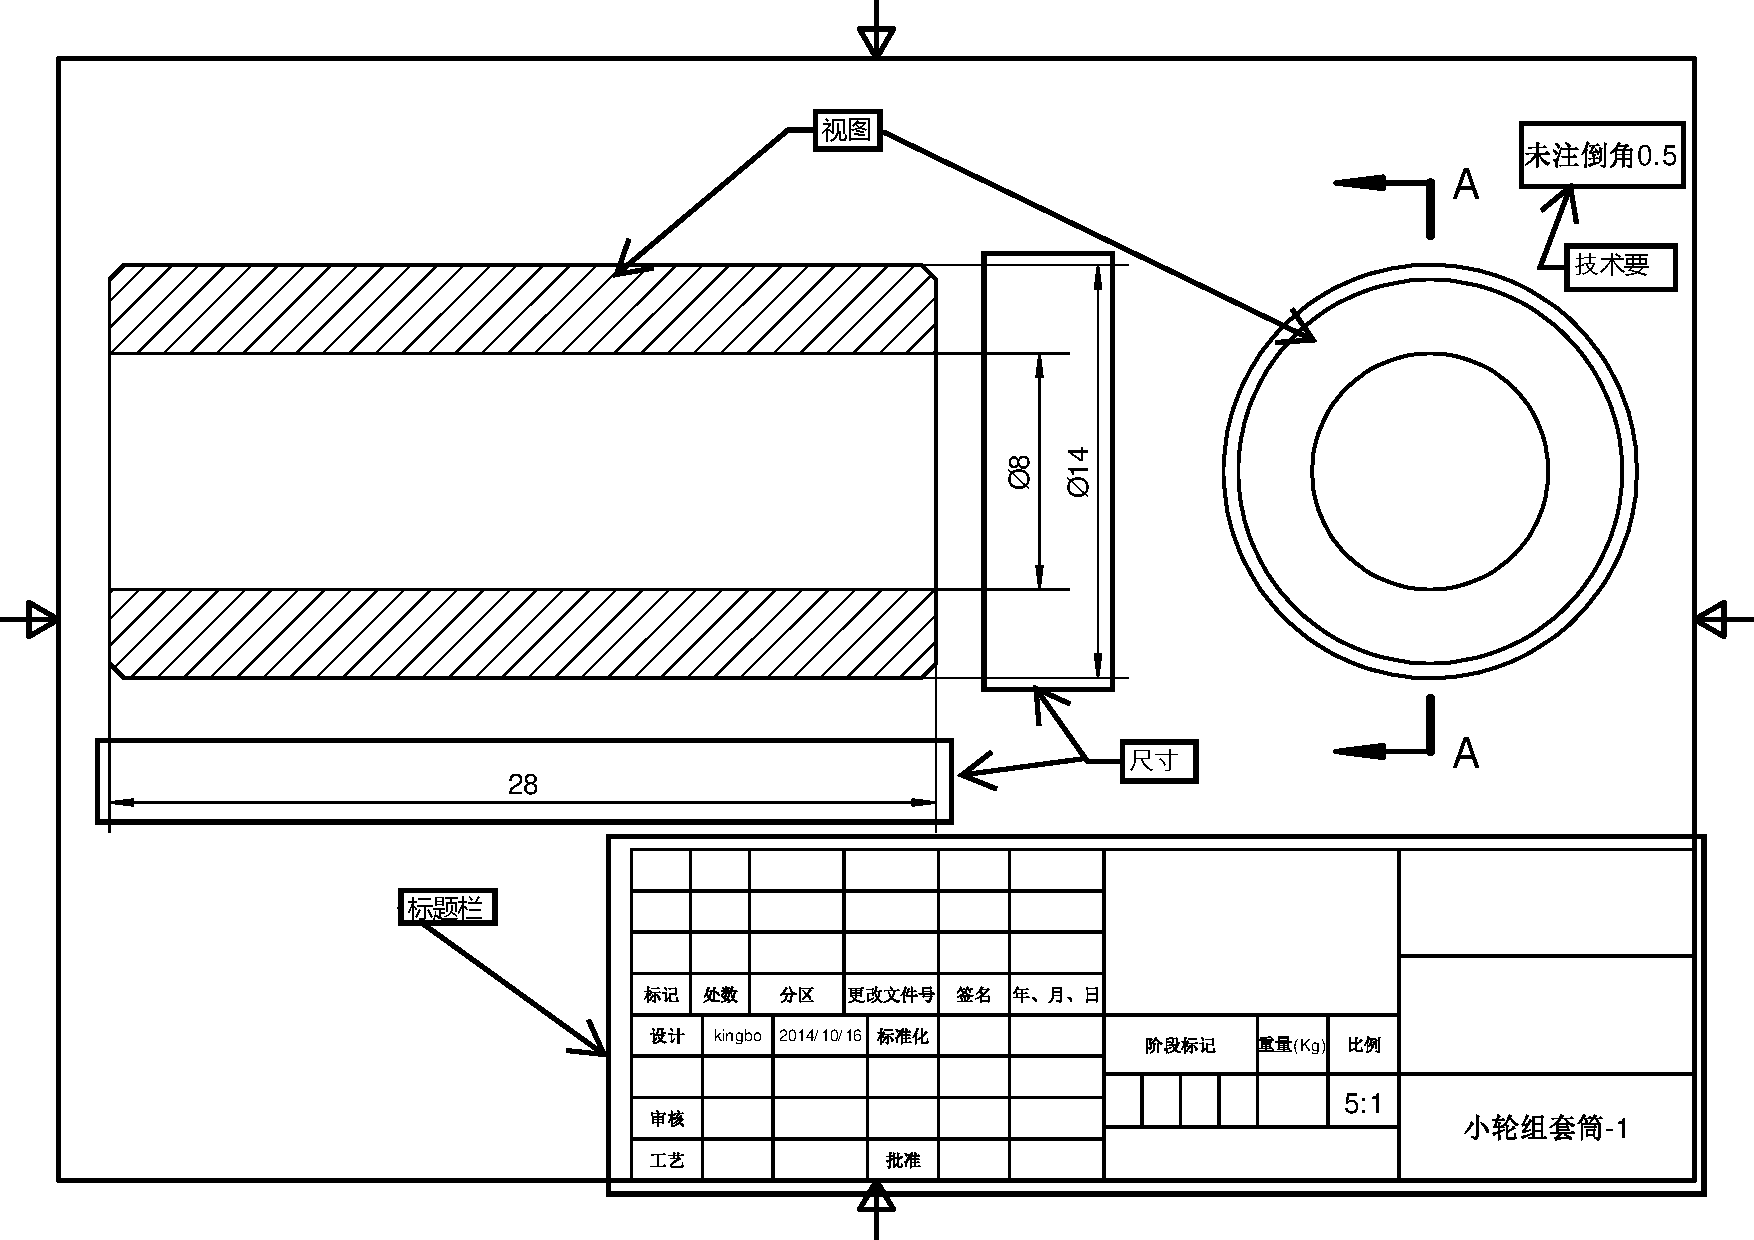
\includegraphics[scale=0.45]{xiaoluntaotong2.pdf}
\caption{零件图组成部分}\label{fig:xiaoluntaotong2}
\end{figure}
图\ref{fig:xiaoluntaotong2}对图\ref{fig:xiaoluntaotong}所示零件图的各个组成部分进行了标注。
\section{圆柱体视图}
图\ref{fig:xiaoluntaotong}所示零件图中的视图既然是用于表达零件的内外形状的,那么它的立体形状是怎样的呢,如保用AutoCAD构建出它的三维模型呢?要解决这个问题,我们先将图\ref{fig:xiaoluntaotong}所示零件图进行简化,忽略其内部及细微的局部,只研究其中$\phi 14$所对应的部分,简化后的结果如图\ref{fig:yuanzhuti}所示。
\begin{figure}[htbp]
\centering
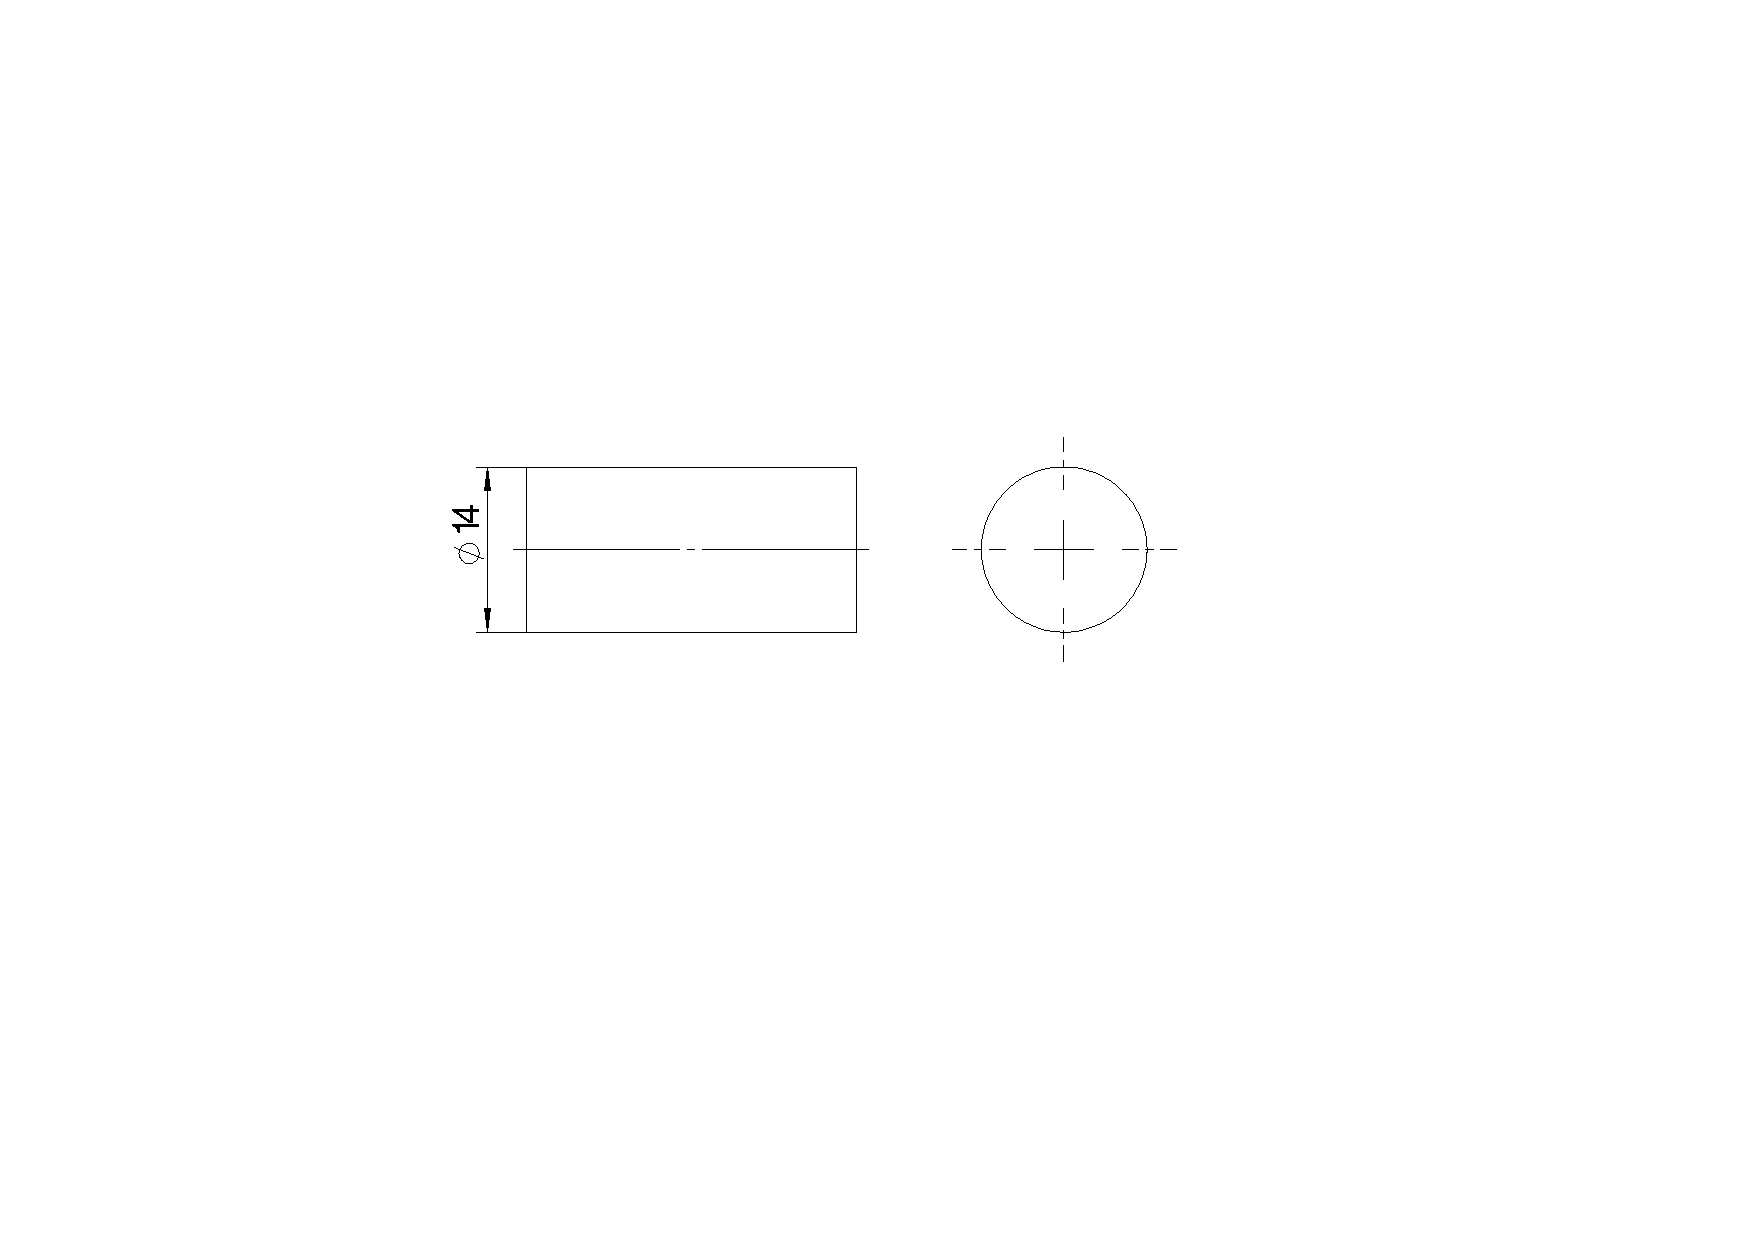
\includegraphics[scale=0.55]{yuanzhuti.pdf}
\caption{套筒外圆柱视图}\label{fig:yuanzhuti}
\end{figure}

那么图\ref{fig:yuanzhuti}所表达的又是什么物体呢?要回答这个问题,我们先将一个圆柱体放置于图\ref{fig:sanweizuobiao}所示的三个相互垂直的三面投影之中,然后从三个方向将圆柱体投影到投影面上,即可得到圆柱体的三面投影,如图\ref{fig:yuanzhutouyin}所示。从圆柱体的三面投影可以看出其中两投影的大小和形状是一样的,均为矩形,仅有一个投影为圆。
\begin{figure}[htbp]
\centering
\subfloat[三维投影面]{\label{fig:sanweizuobiao}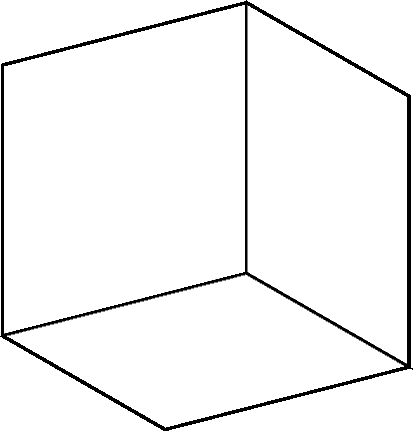
\includegraphics[scale=0.4]{sanweizuobiao.png}}\hspace{30pt}
\subfloat[圆柱体三面投影]{\label{fig:yuanzhutouyin}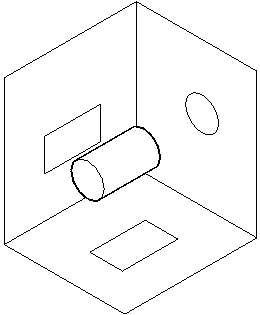
\includegraphics[scale=0.3]{yuanzhutouyin.png}}
\end{figure}

由此可以看出图\ref{fig:yuanzhuti}所示的视图表达的是一个直径为$\phi 14$,长为28的圆柱体,其中符号$\phi$用于表示后面所标注的尺寸是直径。

\endinput
\section{套筒三维模型构建}\label{sec:taotongjianmo}
基于上面的认识和理解,现在可以用AutoCAD来构建套筒的三维模型,具体构建方法是:
\begin{procedure}

\item 启动AutoCAD软件。

启动AutoCAD软件的方法通常有:
\begin{itemize}
\item 双击桌面图标
\includegraphics[scale=0.2]{cadicon.png}。
\item 【开始】$\rightarrow$ 【所有程序】$\rightarrow$【Autodesk】$\rightarrow$【AutoCAD 2014 – 简体中文 (Simplified Chinese)】$\rightarrow$【AutoCAD 2014 – 简体中文 (Simplified Chinese)】。
\end{itemize}
AutoCAD软件启动完成后,将出现图\ref{fig:cadui}所示的软件界面。
\begin{figure}[htbp]
\centering
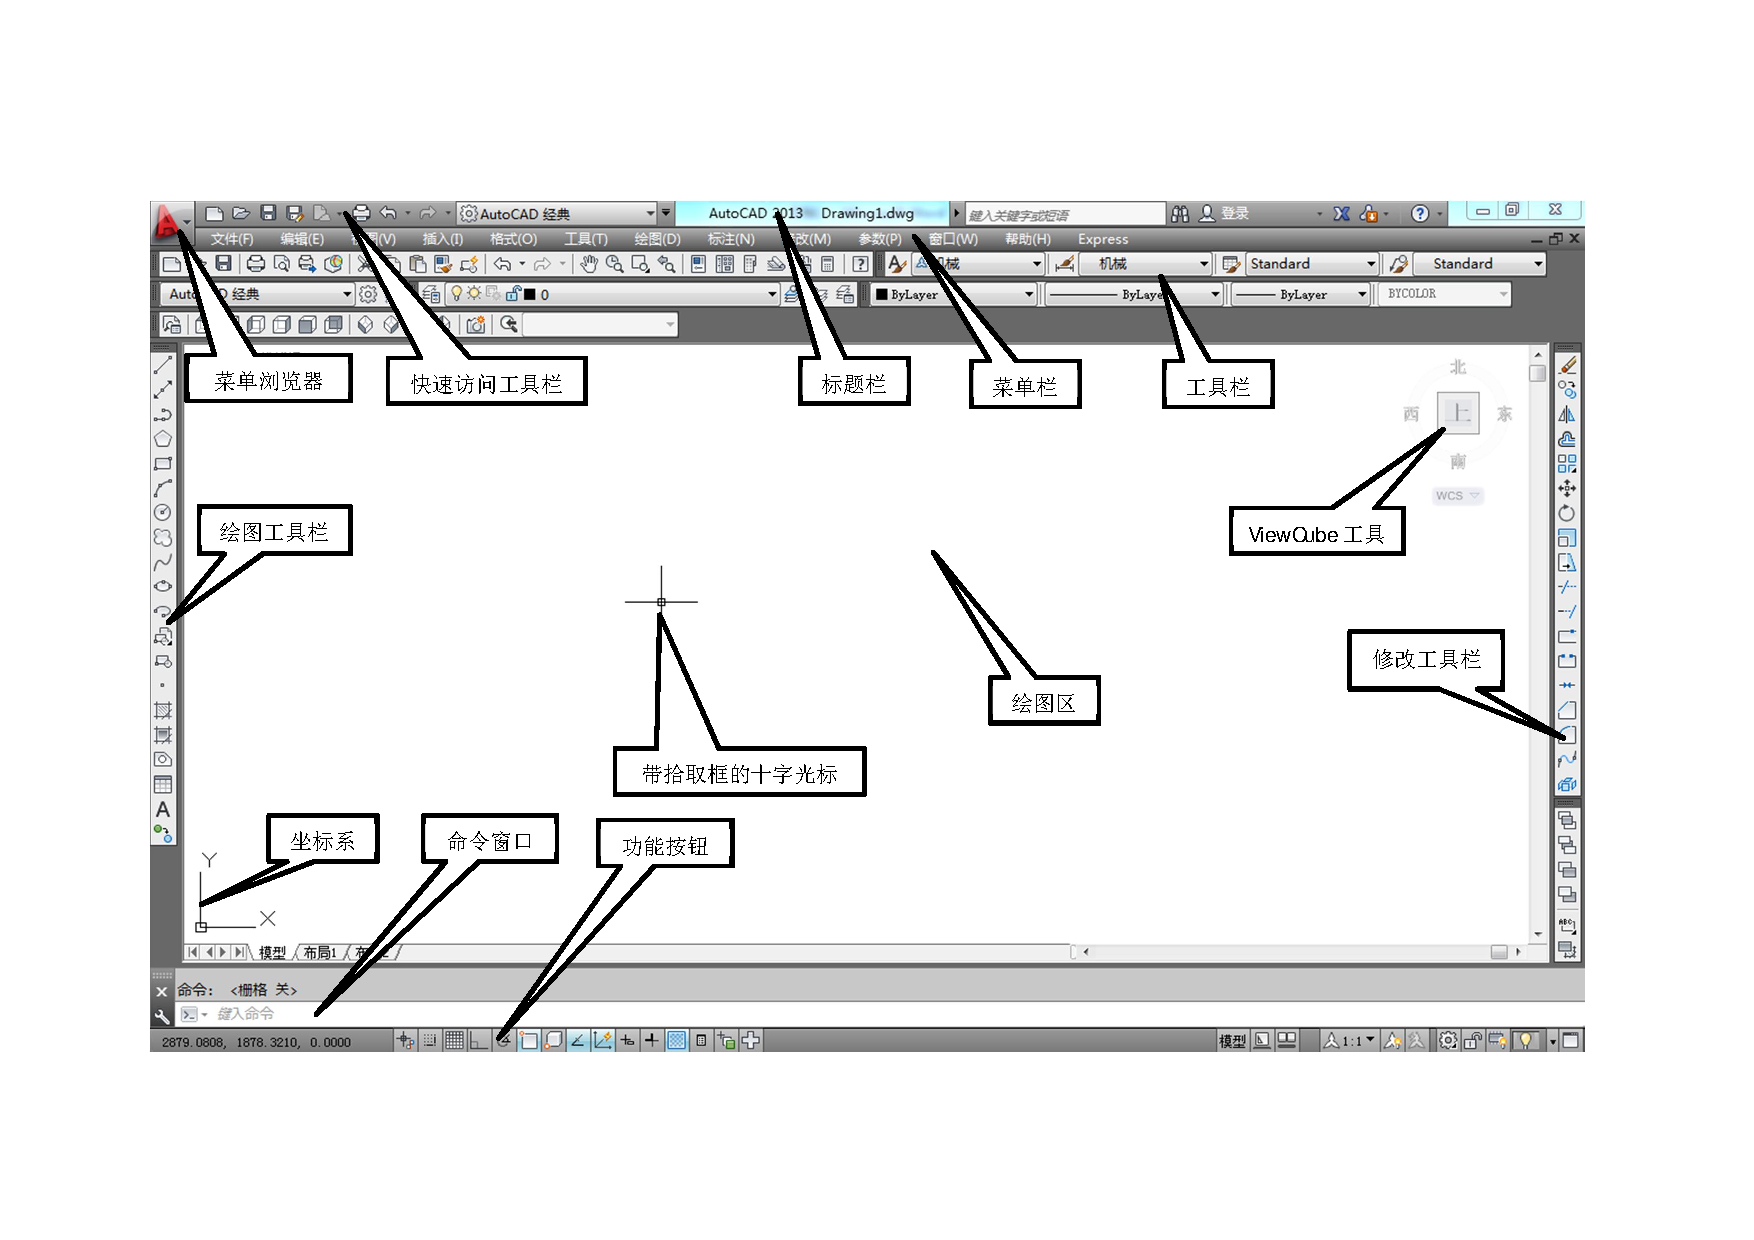
\includegraphics[scale=0.5]{cadui.pdf}
\caption{“AutoCAD经典”工作空间}\label{fig:cadui}
\end{figure}
AutoCAD软件的界面与Word字处理软件的界面非常相似,也是由标题栏、菜单栏、工具栏、绘图区、状态栏等要素构成。不同的是AutoCAD软件的界面在标题栏上还有菜单浏览器和快速访问工具栏;绘图区的左下方有坐标系,右上方有ViewCube工具,左边有绘图工具栏,右边有编辑工具栏;状态栏的上方有命令窗口;状态栏中有功能按钮。

\item 将视图切换为左视图。

AutoCAD启动后默认的视图方向是俯视图方向,而套筒零件的特征图位于左视图方向,为使套筒零件的三维模型与纸方向一致,需要将AutoCAD的视图方向切换为左视图方向。实现左视图切换的方法有:
\begin{itemize}
\item 键盘输入-VIME\index{-view,视图} 或-V,选择【正交】选项中的【左视】项。
\item 键盘输入-VIME,并输入left。
\item 【视图】$\rightarrow$【三维视图】$\rightarrow$【左视图】。
\item 【视图】$\triangleright$【左视】图标
\includegraphics[scale=0.6]{lefttool.png}。
\end{itemize}
同理,如果要将视图切换为其它视图方向,其操作方法与切换左视图的方法是一致的,只是需要将“左视”换成其它视图方向即可。例如要将视图方向切换为俯视图方向则将上述方法中的【左视】改为【俯视】。

\begin{lstlisting}
命令: -VIEW
输入选项 [?/删除(D)/正交(O)/恢复(R)/保存(S)/设置(E)/窗口(W)]: left
\end{lstlisting}

\yaodian{结合能够显著表达物体特征的视图选择AutoCAD的三维视图方向,将有助于三维模型的构建。}

\item 构建外圆柱
在AutoCAD中,创建圆柱体需要用到圆柱体命令,通常启动【圆柱体】命令的方法有:
\begin{itemize}
\item 键盘输入CYLINDER\index{cylinder,圆柱体}或CYL。
\item 【绘图】$\rightarrow$【建模】$\rightarrow$【圆柱体】。
\item 【建模】$\triangleright$【圆柱体】图标
\includegraphics[scale=0.6]{cylinder.png}。
\end{itemize}
在图\ref{fig:commandline}所示的命令行窗口中输入CYLINDER命令,并回车或按空格键结束命令。结束命令输入后,绘图区中的光标形状由带拾取框的十字光标“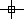
\includegraphics[scale=0.8]{guangbiao1} ”变成十字形光标“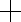
\includegraphics[scale=0.6]{guangbiao2}”,表示此时AutoCAD进入了绘图状态。
\begin{figure}[htbp]
\centering
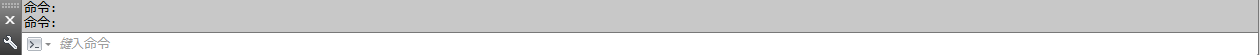
\includegraphics[scale=0.35]{commandline.png}
\caption{AutoCAD命令行}\label{fig:commandline}
\end{figure}

\yaodian{AutoCAD命令行是重要的信息窗口,是正确绘图的关键。初学者应多关注命令行的提示。}
\begin{lstlisting}
命令: _CYLINDER
\end{lstlisting}
接下来命令提示行中会提示,指定圆柱体的底面中心点或者绘图选项。
\begin{lstlisting}
指定底面的中心点或 [三点(3P)/两点(2P)/切点、切点、半径(T)/椭圆(E)]:
\end{lstlisting}
看到上述提示后,可以用鼠标在绘图区中任意单击一下,以完成底面中心点的指定,也可能输入其它选项来指定底面。

接下来,命令提示输入底面的半径,此时根据$\phi 14$直径尺寸计算得到半径应该是7,因此直接从键盘上输入数字7并按空格键或回车键结束半径的指定。如果要指定直径则需要在指定半径的提示下,输入选项字母D来进入指定直径状态。
\begin{lstlisting}
指定底面半径或 [直径(D)]: 7
\end{lstlisting}
最后,命令提示指定圆柱体的高度,此时从键盘上输入数字28,并按回车或空格键结束高度指定。
\begin{lstlisting}
指定高度或 [两点(2P)/轴端点(A)]: 28
\end{lstlisting}
此时,绘图区的光标切换为带拾取框的十字光标,表示AutoCAD当前处于非绘图命令状态。
\item 将视图方向切换为西南等轴测。
\begin{lstlisting}
命令: -VIEW
-VIEW输入选项 [?/删除(D)/正交(O)/恢复(R)/保存(S)/设置(E)/窗口(W)]:  swiso
\end{lstlisting}
完成视图切换后,可以看到图\ref{fig:taotong1} 所示的结果。
\begin{figure}[htbp]
\centering
\subfloat[]{\label{fig:taotong1}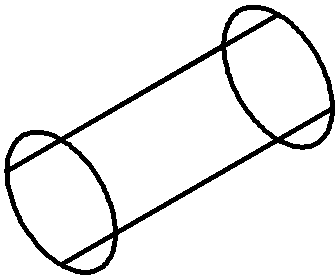
\includegraphics[scale=0.3]{taotong1.png}}\hspace{20pt}
\subfloat[]{\label{fig:centerselect}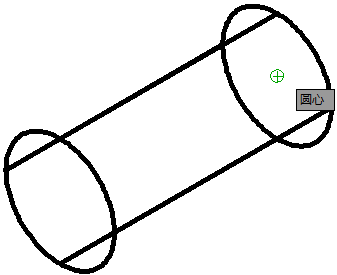
\includegraphics[scale=0.3]{centerselect.png}}\hspace{20pt}
\subfloat[]{\label{fig:taotong2}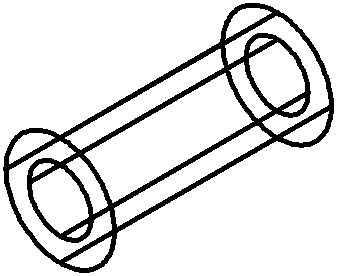
\includegraphics[scale=0.3]{taotong2.png}}
\caption{构建圆柱体}
\end{figure}

\item 构建内圆柱
\begin{lstlisting}
命令: _CYLINDER
指定底面的中心点或 [三点(3P)/两点(2P)/切点、切点、半径(T)/椭圆(E)]:
\end{lstlisting}
当命令提示指定底面圆心时,为保证我们所绘制的$\phi 8$圆柱与$\phi 14$圆上下端面对齐并且同轴,需要应用AutoCAD的对象后捕捉方式来选取$\phi 14$圆底端面的圆心作为$\phi 8$圆柱底端面的圆心。其具体操作方法是:将鼠标移至图\ref{fig:centerselect}所示的位置,直到出现图示的圆心标记和提示,然后单击鼠标左键确定圆柱体的圆心,并按下面的提示完$\phi 8$圆柱体的构建。
\begin{lstlisting}
指定底面半径或 [直径(D)] <7.0000>: 4
指定高度或 [两点(2P)/轴端点(A)] <28.0000>:
\end{lstlisting}

\yaodian{合理使用捕捉是实现精确绘图和快速绘图的重要方法之一。}

\item 进行差集操作,制作内孔

由于前面构建的是两个实体的圆柱体,因此并没有真构成套筒零件所需要的孔,而实现孔的构建则需要从$\phi 14$的圆柱体中去除一个$\phi 8$的圆柱体,要实现这一目标,需要用到实体编辑中的【差集】命令,其启动方法有:
\begin{itemize}
\item 键盘输入SUBTRACT\index{subtract,差集}或SU。
\item 【修改】$\rightarrow$【实体编辑】$\rightarrow$【差集】。
\item 【实体编辑】$\triangleright$【差集】图标
\includegraphics[scale=0.7]{subtracttool.png}。
\end{itemize}
\begin{figure}[htbp]
\centering
\subfloat[]{\label{fig:subtractselect}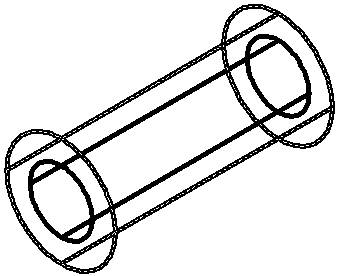
\includegraphics[scale=0.3]{subtractselect.png}}\hspace{40pt}
\subfloat[]{\label{fig:subtractselect1}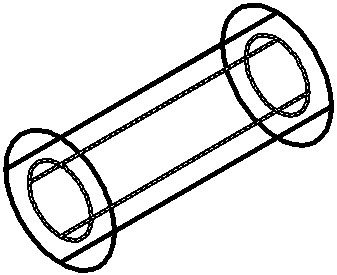
\includegraphics[scale=0.3]{subtractselect1.png}}
\caption{差集操作}
\end{figure}
\begin{lstlisting}
命令: SUBTRACT
选择要从中减去的实体、曲面和面域...
\end{lstlisting}
输入SUBTACT命令后,提示选择要从中减去的实体,同时绘图区的鼠标形状变为矩形小方框“
\includegraphics[scale=0.8]{selectobject.png}”,表示进入选择对象状态,此时按照图\ref{fig:subtractselect}所示选择$\phi 14$的圆柱体作为要从中减去的对象,并按回车或空格键结束选择。
\begin{lstlisting}
选择对象: 找到 1 个
选择对象:  选择要减去的实体、曲面和面域...
\end{lstlisting}
结束从中减去实体选择后,命令提示选择要减去的实体,此时按照图\ref{fig:subtractselect1}所示选择$\phi 8$圆柱体作为要选择的实体,并按驾车可空格键结束选择。
\begin{lstlisting}
选择对象: 找到 1 个
选择对象:
\end{lstlisting}
\item 进行倒角操作
至此,已经完成了套筒的整体部分的构建,还剩下两个倒角没有完成,在AutoCAD中完成三维立体倒角边构建的命令是“倒角边”,其启动方法有:
\begin{itemize}
\item 键盘输入CHAMFEREDGE\index{charmferedge,倒角边}。
\item 【修改】$\rightarrow$【实体编辑】$\rightarrow$【倒角边】。
\item 【实体编辑】$\triangleright$【倒角边】图标
\includegraphics[scale=0.6]{chamferedge.png}。
\end{itemize}

\begin{lstlisting}
命令: CHAMFEREDGE
距离 1 = 1.0000,距离 2 = 1.0000
\end{lstlisting}
启动完倒角边命令后,命令会提示当前的倒角边距离的默认值,并提示选择要倒角的边,此时按照图\ref{fig:chamferedgeselect}所示选择要倒角的一条边,选择完成后会自动生成倒角预览。
\begin{figure}[htbp]
\centering
\subfloat[]{\label{fig:chamferedgeselect}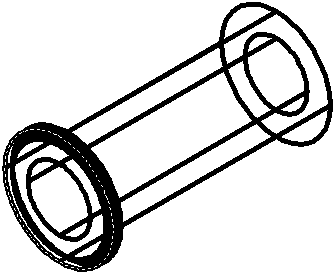
\includegraphics[scale=0.3]{chamferedgeselect.png}}\hspace{20pt}
\subfloat[]{\label{fig:chamferedgeselect1}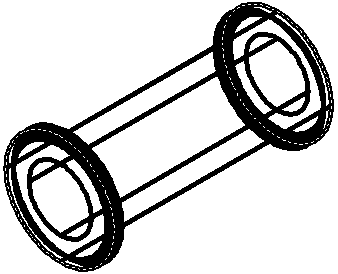
\includegraphics[scale=0.3]{chamferedgeselect1.png}}
\hspace{20pt}
\subfloat[]{\label{fig:chamferedgeresult}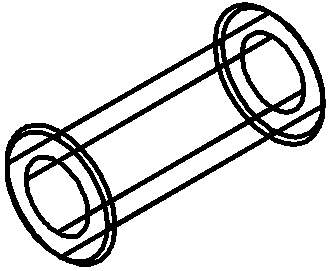
\includegraphics[scale=0.3]{chamferedgeresult.png}}
\caption{倒角边操作}
\end{figure}
\begin{lstlisting}
选择一条边或 [环(L)/距离(D)]:
\end{lstlisting}
接下来,按照图\ref{fig:chamferedgeselect1}所示,选择另一条要倒角的边。
\begin{lstlisting}
选择同一个面上的其他边或 [环(L)/距离(D)]:
\end{lstlisting}
套筒零件只有两个倒角边,因此选择倒角边至此结束,但是系统默认值并不是需要的倒距离,故需要选择距离(d)进行修改。
\begin{lstlisting}
选择同一个面上的其他边或 [环(L)/距离(D)]:d
\end{lstlisting}
最后将两个倒角距离均设置成为0.5,并用回车键接受,其结果如图\ref{fig:chamferedgeresult}所示。
\begin{lstlisting}
指定基面倒角距离或 [表达式(E)] <1.0000>: 0.5
指定其他曲面倒角距离或 [表达式(E)] <1.0000>: 0.5
按 Enter 键接受倒角或 [距离(D)]:
\end{lstlisting}
\item 进行着色
\begin{figure}[htbp]
\centering
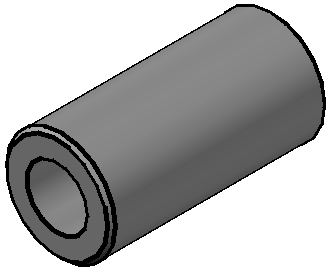
\includegraphics[scale=0.6]{taotonglititu.png}
\caption{套筒三维模型}\label{fig:taotonglititu}
\end{figure}
最后,将完成套筒三维模型以灰度方式的视觉样式进行着色,以使得三维模型看起更加真实。启动灰度视觉样式的方法有:
\begin{itemize}
\item 键盘输入 VSCURRENT\index{vscurrent,视觉样式}或VS,并输入G选项。
\item 【视图】$\rightarrow$【视觉样式】$\rightarrow$【灰度】。
\end{itemize}
\begin{lstlisting}
命令: vscurrent
输入选项 [二维线框(2)/线框(W)/隐藏(H)/真实(R)/概念(C)/着色(S)/带边缘着色(E)/灰度(G)/勾画(SK)/X 射线(X)/其他(O)] <二维线框>: G
\end{lstlisting}
完成灰度视觉样式切换后,其结果如图\ref{fig:taotonglititu}所示。

\item 保存模型

将建立好的套筒三维模型保存为“小轮组套筒.dwg”,AutoCAD中保存文件的方法有:
\begin{itemize}
\item 键盘输入SAVE\index{save,保存}或SAVEAS\index{saveas,另存为}。
\item 键盘输入\fbox{Ctrl}+\fbox{S}。
\item 【文件】$\rightarrow$【保存】或【另存为】。
\item 【工具栏】$\triangleright$【保存】图标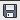
\includegraphics[scale=0.6]{savetool.png}。
\end{itemize}
调用保存命令后,会弹出图\ref{fig:saveasdialog}所示的文件保存对话框,此时在文件名处输入“小轮组套筒.dwg”,并单击保存。
\begin{figure}[htbp]
\centering
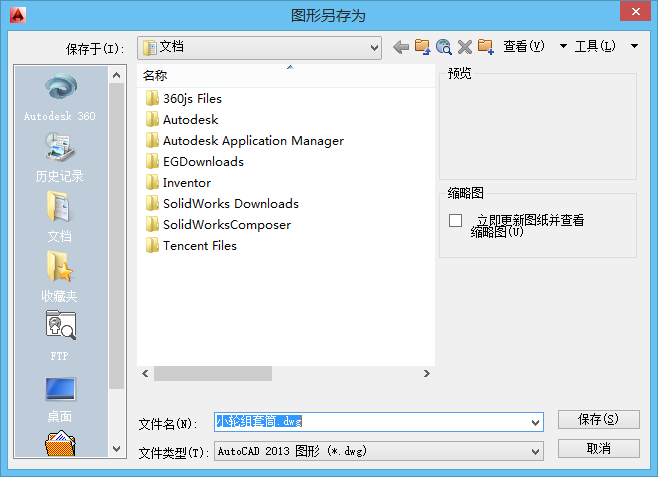
\includegraphics[scale=0.6]{saveasdialog.png}
\caption{保存文件对话框}\label{fig:saveasdialog}
\end{figure}
\end{procedure}

\endinput
\section{理解视图}
为什么图\ref{fig:xiaoluntaotong}所示的零件图能够唯一也表达\ref{fig:taotonglititu}所示的套筒零件呢,为什么需要两视图呢,一个视图能不能够表达呢,要回答这个问题,需要进一步了解一些与视图相关的知识。
\subsection{视图的概念}
\begin{figure}[htbp]
\centering
\subfloat[斜投影法]{\label{fig:xietouyinfa}
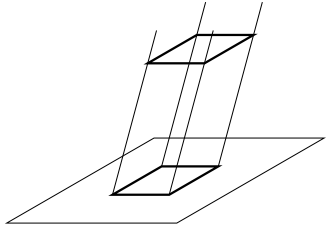
\includegraphics[scale=0.4]{xietoying.png}
}\hspace{30pt}
\subfloat[正投影法]{\label{fig:zhentouyinfa}
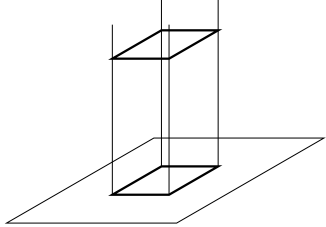
\includegraphics[scale=0.4]{zhengtouying.png}
}
\caption{平行投影法}\label{pingxingtouyin}
\end{figure}

 在图\ref{fig:xiaoluntaotong}所示的套筒零件图中,位于左边的图形称之为主视图,其表达式为全剖视图,关于全剖视图的概念及画法将在后面予以介绍。主视图清晰的表达了套筒零件的长度及内外结构。而位于右边的视图称之为左视图,它清楚地显示套筒零件为回转体类零件。

要理解什么是视图,首先需要了解投影的概念。投影是物体在阳光或灯光下所产生的影子。由于影子只能够表现物体轮廓而不能够表现物体的内部结果,工程实际中将物体内外空间几何元素加以抽象,并用不同的线型进行表示,实现物体内外细节的表达,从而形成的比较完备的、实用的投影方法。投影法分为中心投影法和平行投影法两类。所有投影线都互不平行且汇聚于点的投影法称为中心投影法。中心投影法主要用于绘制效果比较逼真的建筑或产品立体图。图\ref{pingxingtouyin}所示的投影法是平行投影法,从中可以看出其所有的投影线都是相互平行的,其中投影线倾斜于投影面则为斜投影,投影线垂直于投影面则为正投影法。工程中将用正投影法绘制的物体图形称为视图。
\begin{figure}[htbp]
\centering
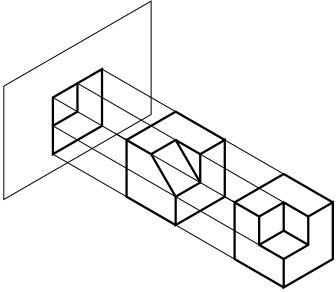
\includegraphics[scale=0.4]{buweiyi.png}
\caption{一个投影面不能确定物体在空间中的形状和位置}\label{fig:singleprojection}
\end{figure}
\subsection{三视图的形成}

\begin{figure}[htbp]
\centering
\subfloat[物体在三面投影中的投影]{\label{fig:threeviewprojection}
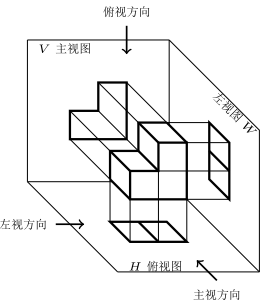
\includegraphics[scale=0.4]{wutisanmiantouying.png}}
\hspace{30pt}
\subfloat[三个投影面的展开]{\label{fig:threeviewzhankai}
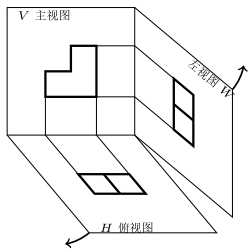
\includegraphics[scale=0.45]{touyingzhankai.png}}


\subfloat[展开后的三视图]{\label{fig:threeview}
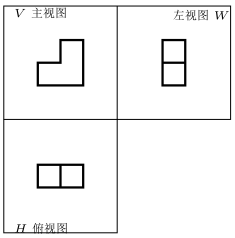
\includegraphics[scale=0.45]{zhankairesult.png}}
\hspace{30pt}
\subfloat[最终三视图]{\label{fig:threeviewguilu}
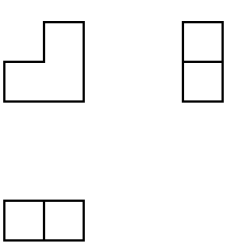
\includegraphics[scale=0.45]{sanshituresult.png}}
\caption{三视图的形成}
\end{figure}
了解完视图的概念后,让们来探讨一个视图能不能够准确地表达出物体的形状这个问题,首先让我们来看一下图\ref{fig:singleprojection}所示的投影。从图\ref{fig:singleprojection}中,我们可以看出不同的形状的物体在同一个视图投影面内具有相同的视图表示。之所以如此,主要是因为仅用一个视图只能反映物体两方向的尺寸,而空间物体需要用长宽高三个方向的尺寸帮能够将其大小形状完整清晰地表达出来。在没有尺寸标注的辅助的情况下,要解决投影只能够表达物体两个尺寸方向的问题,我们需要将物体向多个投影面进行投影,通过多个投影视图来实现物体上下、左右、前后各部分的形状和大小完整表达。在工程零件图中,通常都会使用两个或三个视图来表达一个零件。当然对于简单的轴类零件也经常使用一个视图来表达,对于特别复杂的零件还需要使用更多的辅助视图加以表达。但无论使用多少个视图,三视图是基本的零件图表达方式。下面,我们就来了解一下三视图的形成过程。




为此,我们需要根据国家标准规定,选三个相互垂直的投影面构成图\ref{fig:threeviewprojection}所示的三投影面体系。在三视图投影体系中,正对观察者的投影面称为正平面,用$V$表示。水平放置的投影面称水平面,用$H$表示。侧立的投影面称为侧平面,用$W$表示。将物体放置于三视图投影体系中,将其由前向后投影所得的$V$面视图称为主视;将其由上向下投影所得的$H$面视图称为府视图;将物体由左向右投影所得的$W$面视图称为左视图。最后,按照国家标准,以图\ref{fig:threeviewzhankai}所示方式展开,即以$V$面视图为基准,$H$面绕$V$面与$H$面的交线所形成的$X$轴向下旋转$90^o$;$W$面绕$V$面与$W$面的交线所形成的$Z$轴向右旋转$90^o$,使$V$、$H$、$W$面处于同一个平面内,如图\ref{fig:threeview}所示。展开后的三视图既不需要画边框和投影轴,也不需要标视图名称,如图\ref{fig:threeviewguilu}所示。

\subsection{三视图投影规律}
既然表达一个零件需要多个视图,那么这些视图之间就需要遵循一定规律,才能够准确的表示物体各个组成部分之间的关系。而视图之间所遵循的规律则称之为对应关系。图\ref{fig:threeviewguanxi}标识了三个视图之间的对应关系和视图所能表达的方位。从图中,我们可以得出:主视图反映物体的上下和左右关系,即反映物体的长和高;俯视图反映物体的左右和前后关系,即反映物体的长和宽;左视图反映物体的上下和前后,即反映物体的高和宽。因此,三视图的投影规律为:
\begin{itemize}
\item 主、俯视图长对正;
\item 主、左视图高平齐;
\item 俯、左视图宽相等。
\end{itemize}
\begin{figure}[htbp]
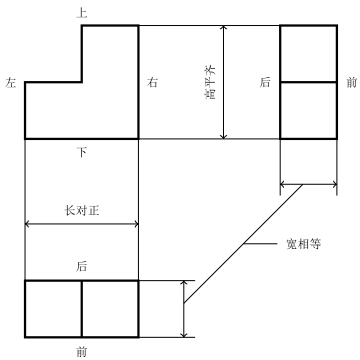
\includegraphics[scale=0.6]{touyingguilu.png}
\caption{三视图投影规律}\label{fig:threeviewguanxi}
\end{figure}
三视图的投影规律不仅适用于物体整体之间的投影,也适用于空间中的点、线面。同时它也是画图和读图的基础规则。由此可知,图\ref{fig:xiaoluntaotong}所示的套筒零件图中,主视图中$\phi 14$尺寸所标法的图线与左视图中的大圆处于同一条水平线上,符合高平齐的对应关系,表达了套筒的外形整体为圆柱体,与此类似,$\phi 8$则表达了套筒的内孔,紧邻大圆的中间圆则表达了倒角。

\endinput
\section{检验结果}
在了解了相关的视图知识后,让我们来简单地检验下套筒零件的三维模型的投影是不是与零件图的视图基本一致的。为什么说是基本一致呢,主要是因为接下来的检验方法仅仅是在AutoCAD的模型空间中,用切换视图方向的方法进行观察套筒的三维模型,其表现方式类似于生活中的影子,并不符合工程图的制图规范。

\begin{procedure}
\item 将视觉样式切换为二维线框

在\ref{sec:taotongjianmo}节中,为了便于看到真实的套筒零件三维模型,我们将视觉样式设置成了灰度。在本节中为了方便观察不同方向的视图,我们需要将视觉样式设置为二维线框方式。

\begin{lstlisting}
命令: VSCURRENT
输入选项 [二维线框(2)/线框(W)/隐藏(H)/真实(R)/概念(C)/着色(S)/带边缘着色(E)/灰度(G)/勾画(SK)/X 射线(X)/其他(O)] <灰度>: 2
\end{lstlisting}
\item 观察主视图
要观察套筒的主视图,需要将三维视图切换为前视图方向,其切换方法与\ref{sec:taotongjianmo}节中切换左视图的方法基本相同,图\ref{fig:taotongfront} 所示为切换为前视图后的结果。从图中可以看出,整个图形的外形与套筒零件的主视图外形是一致的,主要区别是关于内部结构的表达。

\begin{lstlisting}
命令: -VIEW
输入选项 [?/删除(D)/正交(O)/恢复(R)/保存(S)/设置(E)/窗口(W)]: front
\end{lstlisting}
\item 观察左视图
将视图方向切换为左视图,可以得到图\ref{fig:taotongleft}所示的结果。从图中可以看出,他与套筒的左视图是基本相同。
\begin{lstlisting}
命令: -VIEW
输入选项 [?/删除(D)/正交(O)/恢复(R)/保存(S)/设置(E)/窗口(W)]: left
\end{lstlisting}
\item 观察俯视图
将视图切换为俯视图后,其结果如图\ref{fig:taotongtop}所示,可以看它与主视图方向的一图形是一致的。
\begin{lstlisting}
命令: -VIEW
输入选项 [?/删除(D)/正交(O)/恢复(R)/保存(S)/设置(E)/窗口(W)]: top
\end{lstlisting}
\begin{figure}[htbp]
\subfloat[主视图]{\label{fig:taotongfront}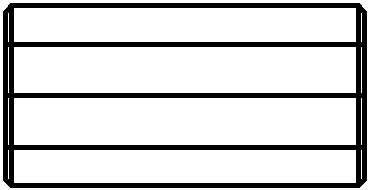
\includegraphics[scale=0.5]{taotongfront.png}}\hspace{15pt}
\subfloat[左视图]{\label{fig:taotongleft}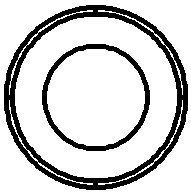
\includegraphics[scale=0.5]{taotongleft.png}}\hspace{15pt}
\subfloat[俯视图]{\label{fig:taotongtop}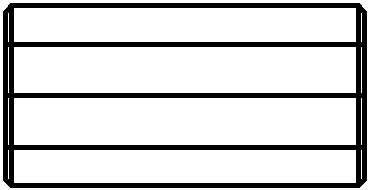
\includegraphics[scale=0.5]{taotongfront.png}}
\end{figure}
\end{procedure}

从上面的简单检验结果来看,我们套筒零件的三维建模是正确。其实,这种简单的检验方法将在AutoCAD的建模过程中会经常用到,尽管他与实际工作图存在一定的差别,但是它的操作步骤简便,能够快速地验证结果,能够有效地辅助三维建模,比较实用。
\endinput
\section{小结}
本章通过套筒零件的三维模型的构建,介绍了利用AutoCAD的圆柱体命令构建套筒的外形实体和内孔实全,并利用并集命令实现孔洞的构建,最后运用倒角边命令来实现三维倒角,整个过程化繁为简。化繁为简一种重要的思维方法。另一个方面,我们还介绍了与套筒三维模型构建的三视图知识,掌握必要的视图知识,是准确构建三维模型的基础,需要在练习中逐步掌握和运用三视图的支应规律,分析零件的重要组成部分。
\endinput
\section*{练习题}
\begin{enumerate}
\item 
\begin{question}
构建图\ref{exerc:exercise1-4}和图\ref{exerc:exercise1-2}  所示物体的三维模型。
\begin{figure}[htbp]
\centering
\begin{floatrow}[2]
\ffigbox{\caption{ }\label{exerc:exercise1-4}}{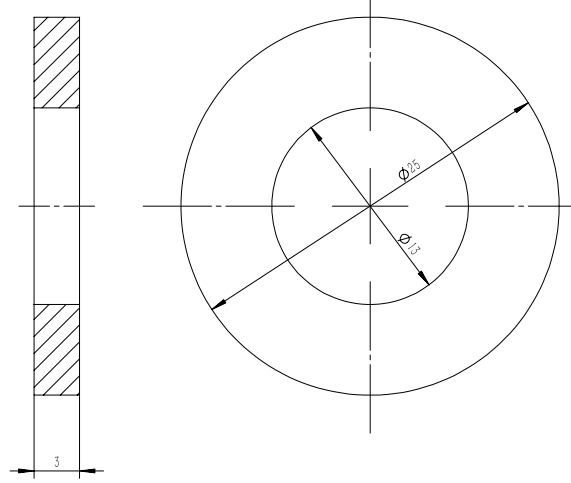
\includegraphics[scale=0.35]{exercise1-4}}
\ffigbox{\caption{ }\label{exerc:exercise1-2}}{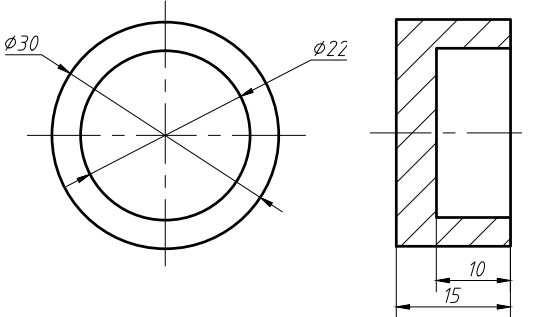
\includegraphics[scale=0.5]{exercise1-2}}
\end{floatrow}
\end{figure}
\end{question}

\item 
\begin{question}
构建图\ref{exerc:exercise1-3}和图\ref{exerc:exercise1-1}  所示物体的三维模型。
\begin{figure}[htbp]
\centering
\begin{floatrow}[2]
\ffigbox{\caption{ }\label{exerc:exercise1-3}}{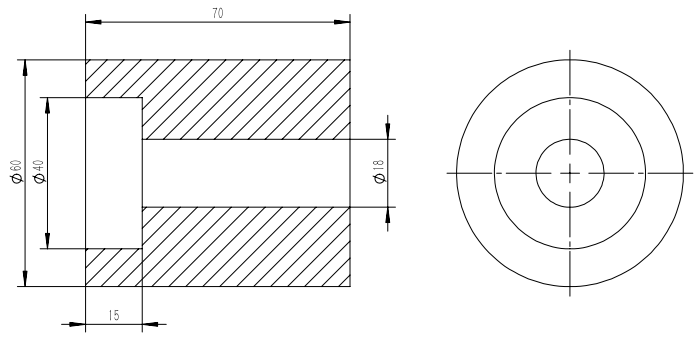
\includegraphics[scale=0.45]{exercise1-3}}
\ffigbox{\caption{ }\label{exerc:exercise1-1}}{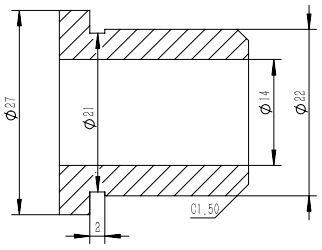
\includegraphics[scale=0.6]{exercise1-1}}
\end{floatrow}
\end{figure}
\end{question}

\item 
\begin{question}
构建图\ref{exerc:exercise1-5} 所示物体的三维模型。
\begin{figure}[htbp]
\centering
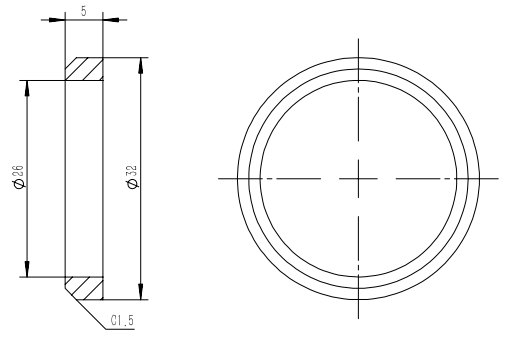
\includegraphics[scale=0.6]{exercise1-5}
\caption{ }\label{exerc:exercise1-5}
\end{figure}
\end{question}
\end{enumerate}
\endinput
%%%%%%%%%%%%%第二章%%%%%%%%%%%%%%%%%%%%%%%
\chapter{轮轴}
\noindent
\begin{figure}[htbp]
\centering
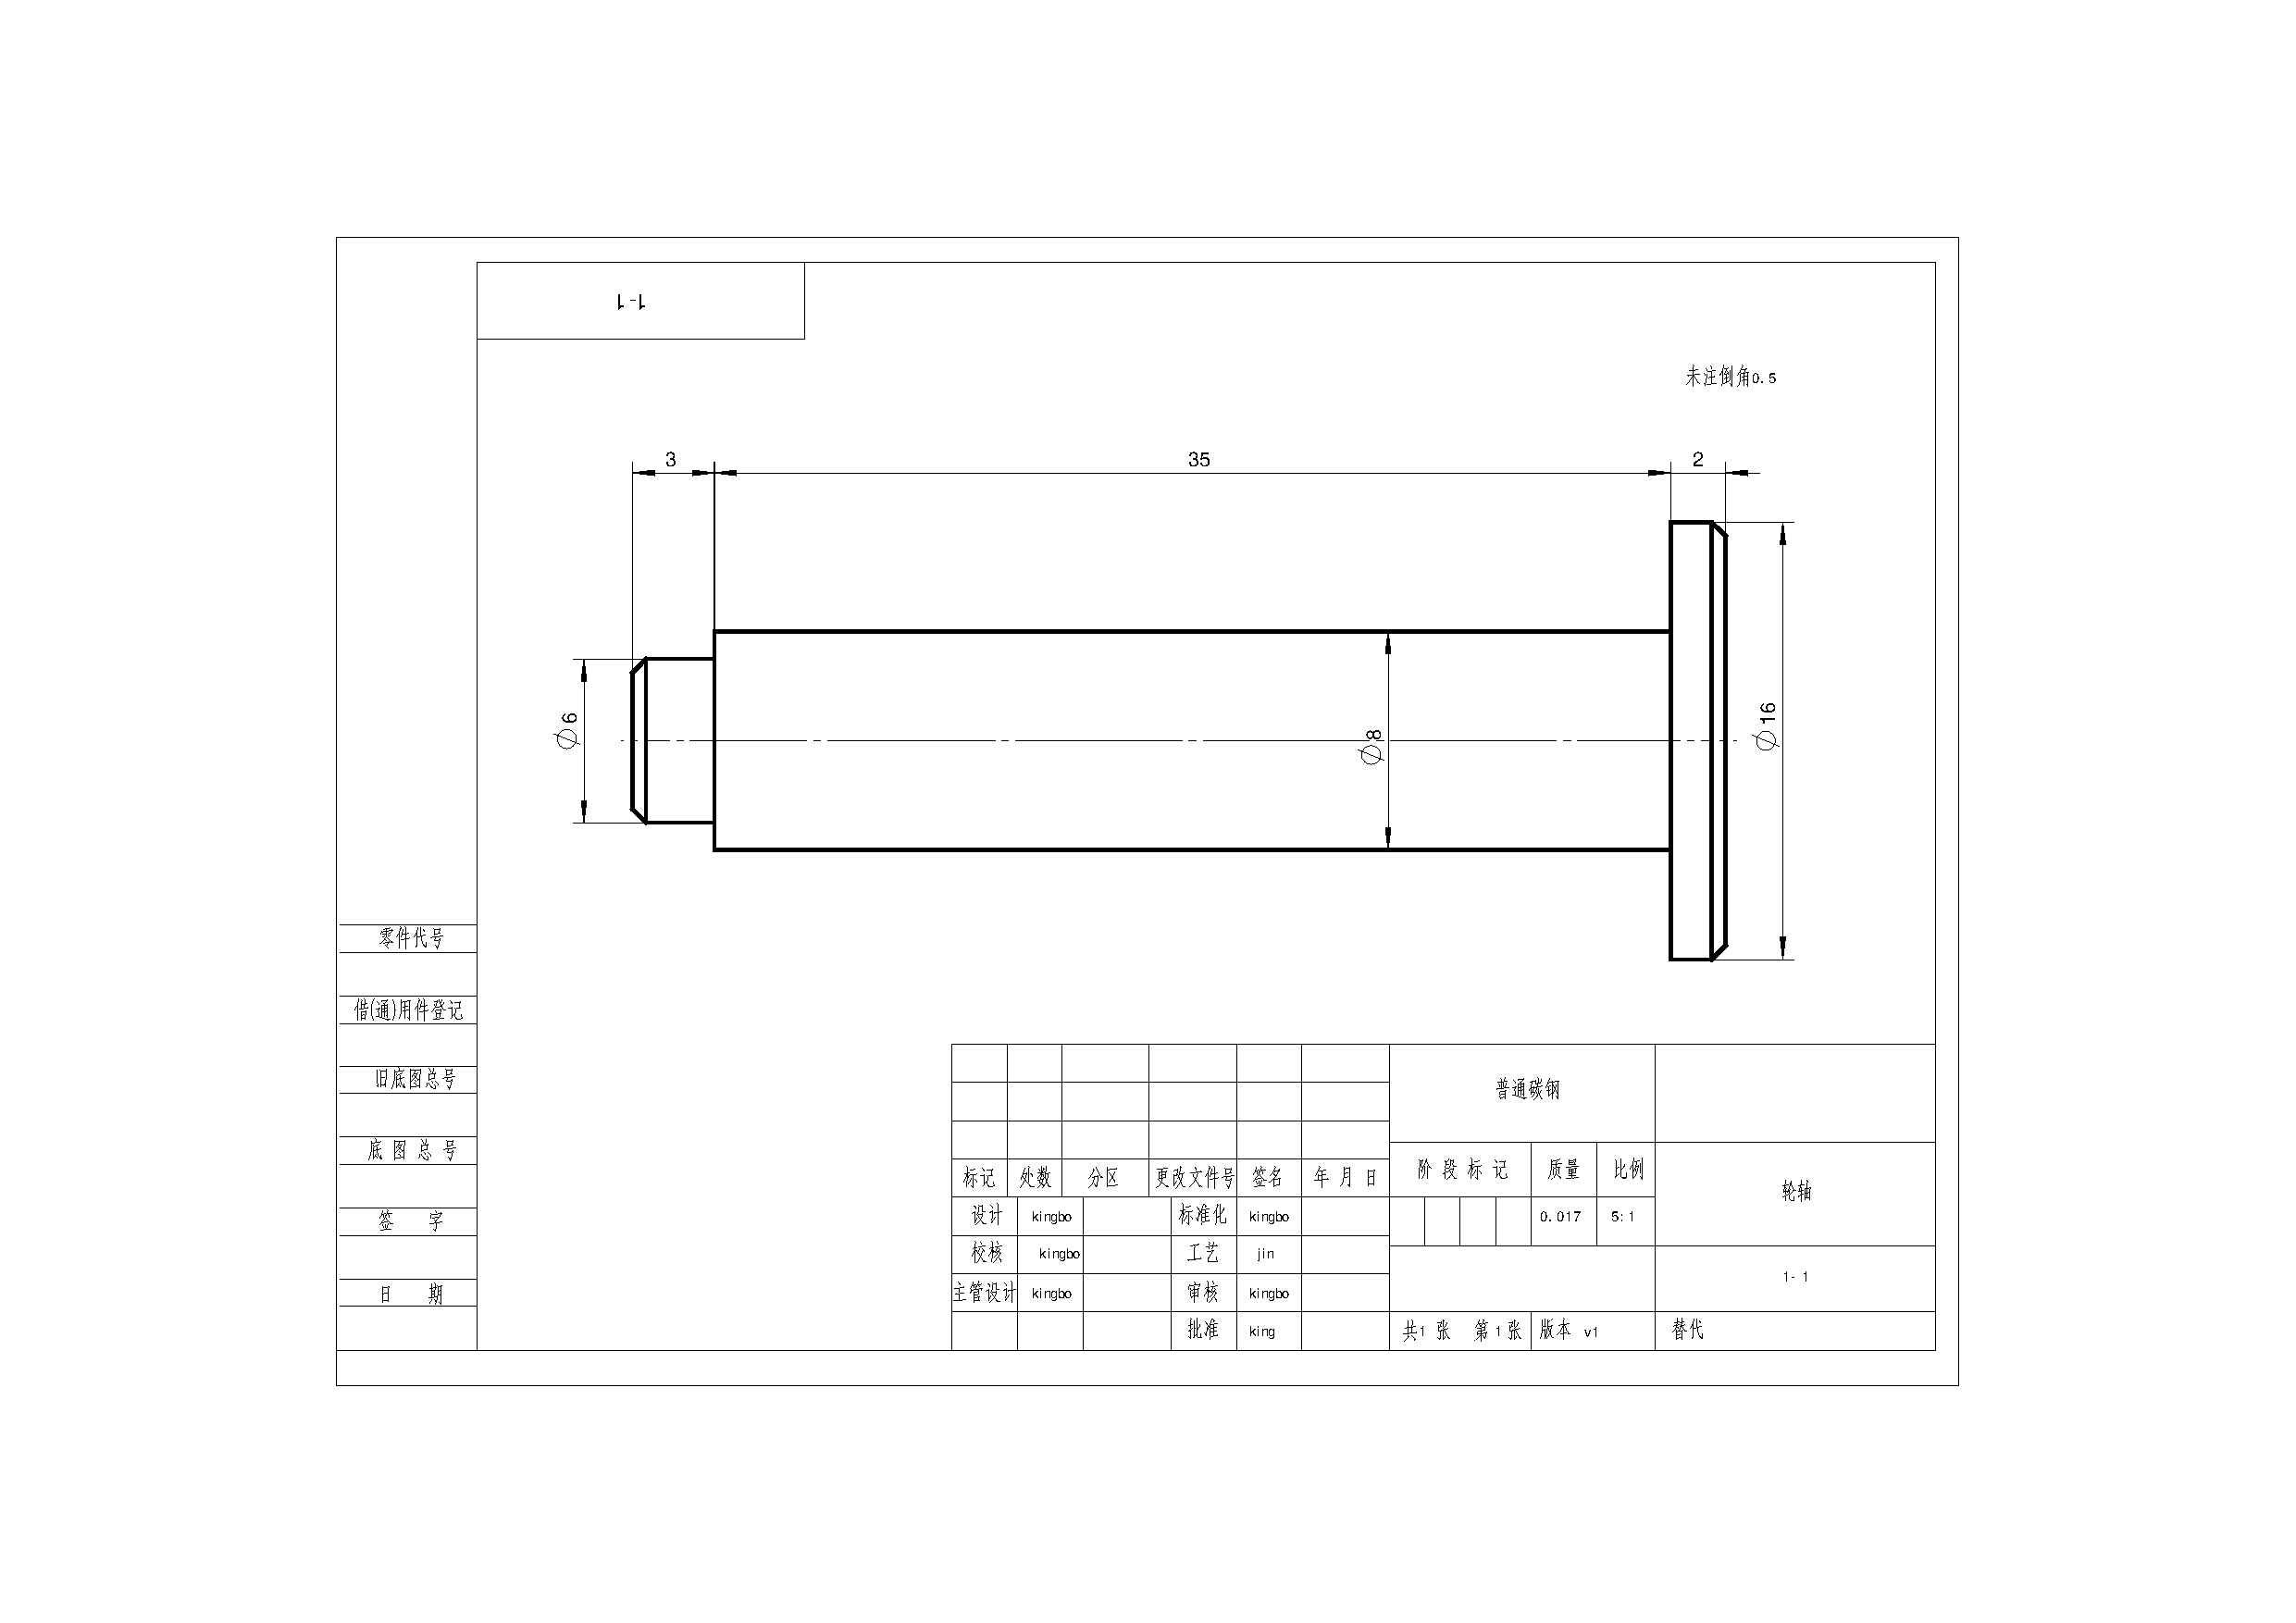
\includegraphics[scale=0.45]{xiaolunzhou.pdf}
\caption{轮轴零件图}\label{fig:xiaolunzhou}
\end{figure}

本简的目标是用AutoCAD制作图\ref{fig:xiaolunzhou}所示轴零件的三维模型,并用布局空间生成该三维模型的主视图,以验证模型的正确性,使学习者进一步理解三维模型与工程零件图之间的关系。因此,本章将讲述以下内容:
\begin{itemize}
	\item 轴零件三维模型的构建
	\item 并集操作
	\item 视图的生成
	\item 图幅和比例的标准
\end{itemize}

\endinput
\section{轴建模过程分析}
图\ref{fig:xiaolunzhou}所示的轴零件由一个主视图构成,根据\ref{sec:lijieshitu}节的知识可知一个视图通常是不能够唯一表达物体的。但仔细观察轴零件图的垂直方向的尺寸标注,可以发现垂直方向尺寸标注的一个共同点是均有表示直径的符号$\phi$,由此可知轴零件的各个组成部分都是圆柱体。 基于\ref{sec:taotongjianmo}节套筒零件的三维建模经验,可以采用以下两种方式进行三维建模。

\yaodian{合理清晰的尺寸标注有助于视图表达。}
\subsection{分段建模}
从图\ref{fig:xiaolunzhou}中可以直观的看出整个轴零件由三段组成,分别是直径$\phi 6$长3的圆柱体、直径$\phi 8$长35的圆柱体和直径$\phi 16$长2的圆柱体。结果如图\ref{fig:zhoufengxi1}所示。
\begin{figure}[htbp]
\centering
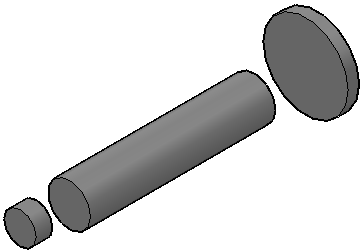
\includegraphics[scale=0.6]{zhoufengxi1.png}
\caption{分段建模}\label{fig:zhoufengxi1}
\end{figure}
\subsection{按包含关系建模}
轴零件整个都是实体,因此可以将两个轴零件看作这样一种包含关系,即$\phi 16$的圆柱体包含了$\phi 8$和$\phi 6$两个圆柱体的部分实体,$\phi 8$的圆柱体包含了$\phi 6$的部分实体。因此,$\phi 8$圆柱体的长度要加上$\phi 16$圆柱体的长度,故长为37。与此类似,可得$\phi 6$圆柱体的长度则为40。结果如图\ref{fig:zhoufengxi2}所示。
\begin{figure}[htbp]
\centering
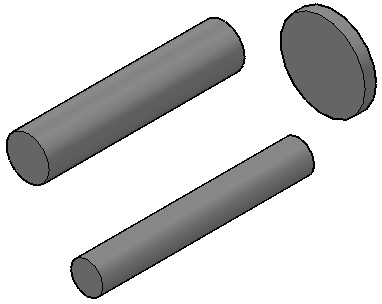
\includegraphics[scale=0.6]{zhoufengxi2.png}
\caption{按包含关系建模}\label{fig:zhoufengxi2}
\end{figure}

对于图\ref{fig:xiaolunzhou}所示的轴零件而言,用分段建模更为直观和直接,但实际中两建模方式并没有优劣之分,应当根据所需建模零件的实际情况灵活地综合运用。
\endinput
\section{轴三维模型构建}

\begin{lstlisting}
命令: -VIEW
输入选项 [?/删除(D)/正交(O)/恢复(R)/保存(S)/设置(E)/窗口(W)]: left
\end{lstlisting}

\begin{lstlisting}
命令: -VIEW
输入选项 [?/删除(D)/正交(O)/恢复(R)/保存(S)/设置(E)/窗口(W)]: swiso
\end{lstlisting}

\begin{lstlisting}
命令: CYLINDER
指定底面的中心点或 [三点(3P)/两点(2P)/切点、切点、半径(T)/椭圆(E)]:
指定底面半径或 [直径(D)]: 8
指定高度或 [两点(2P)/轴端点(A)]: 2
\end{lstlisting}

\begin{lstlisting}
命令: CYLINDER
指定底面的中心点或 [三点(3P)/两点(2P)/切点、切点、半径(T)/椭圆(E)]:
指定底面半径或 [直径(D)] <8.0000>: 4
指定高度或 [两点(2P)/轴端点(A)] <2.0000>: 35
\end{lstlisting}

\begin{lstlisting}
命令: CYLINDER
指定底面的中心点或 [三点(3P)/两点(2P)/切点、切点、半径(T)/椭圆(E)]:
指定底面半径或 [直径(D)] <4.0000>: 3
指定高度或 [两点(2P)/轴端点(A)] <35.0000>: 3
\end{lstlisting}

\begin{lstlisting}
命令:  UNION
选择对象: 指定对角点: 找到 3 个
选择对象:
\end{lstlisting}

\begin{lstlisting}
命令: CHAMFEREDGE
距离 1 = 1.0000,距离 2 = 1.0000
选择一条边或 [环(L)/距离(D)]: d
指定距离 1 或 [表达式(E)] <1.0000>: 0.5
指定距离 2 或 [表达式(E)] <1.0000>: 0.5
选择一条边或 [环(L)/距离(D)]:
选择同一个面上的其他边或 [环(L)/距离(D)]:
按 Enter 键接受倒角或 [距离(D)]:
\end{lstlisting}

\begin{lstlisting}
命令: CHAMFEREDGE
距离 1 = 0.5000,距离 2 = 0.5000
选择一条边或 [环(L)/距离(D)]:
选择同一个面上的其他边或 [环(L)/距离(D)]:
按 Enter 键接受倒角或 [距离(D)]:
\end{lstlisting}

\begin{lstlisting}
命令: VSCURRENT
输入选项 [二维线框(2)/线框(W)/隐藏(H)/真实(R)/概念(C)/着色(S)/带边缘着色(E)/灰度(G)/勾画(SK)/X 射线(X)/其他(O)] <二维线框>: g
\end{lstlisting}

\endinput
\section{轴主视图生成}\label{sec:zhoushitu}
\begin{procedure}
\item 保存轴三维模型的副本

将轴的三维模型另存为“轴视图布局.dwg”。之所以要保存副本,一是为了防止视图布局操作对模型文件的影响,二是可以多次使用。

\yaodian{进行三维模型的视图布局操作之前,保存副本是一个良好的习惯。}

\item 将模型空间切换图纸空间

AutoCAD默认开始工作的空间是模型空间。模型空间是一个无限的三维绘图区域,可以用于制作1:1的二维图或三维模型。AutoCAD的图纸空间则主要用于图形输出准备。在图形空间中可以设置带有标题栏和注释的不同布局。在每个布局中,可以创建显示模型空间的不同视图的布局视口。在布局视口中,可以相对于图纸空间缩放模型空间视图。由此可见图纸空间可以实现形式多样的图形输出方式,模型空间更加灵活。

在AutoCAD中实现由模型空间切换为比较方便,用鼠标单击命令提示窗口上面的选项卡,使其由模型状态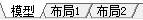
\includegraphics[scale=0.6]{moxinkongjian.png} 切换为布局状态\includegraphics[scale=0.6]{bujukongjian.png} 即可。切换后,会出现图\ref{fig:morenbuju}所示的默认布局。

\begin{figure}[htbp]
\centering
\begin{floatrow}[2]
\ffigbox{\caption{默认布局}\label{fig:morenbuju}}{\includegraphics[scale=0.4]{morenbuju.png}}
\ffigbox{\caption{布局右键菜单}\label{fig:bujurightmeum}}{\includegraphics[scale=0.5]{bujurightmeum.png}}
\end{floatrow}
\end{figure}

\item 修改页面设置

通常默认布局的页面设置并不能够满足实际图纸输出的需求,因此需要修改布局的设置。AutoCAD启动页面设置管理器的方法有:
\begin{itemize}
\item 键盘输入 paggesetup\index{pagesetup,页面设置管理器}。
\item 【文件】$\rightarrow$【页面设置管理器】$\rightarrow$【并集】。
\item 在布局选项卡上右击鼠标,弹出图所示\ref{fig:bujurightmeum}菜单,然后选择【页面设置管理器】项。
\end{itemize}

\begin{lstlisting}
命令:pagesetup
\end{lstlisting}

页面设置管理器启动后,会弹出图\ref{fig:pagesetup}所示对话框。此时,单击修改按钮,弹出图\ref{fig:pagesetupdetail}所示的页面设置对话框。然后按照图\ref{fig:pagesetupdetail}的设置,将打印机绘图设备修改为“DWG TO PDF.pc3”,图纸尺寸设置为ISO A4(210.00x297.00毫米),其它参数保持不变。实际工作中应该打印机绘图设备设置为能够正常输出图形的真实打印机,才能够真正实现图形的打印输出。本书的设置是将AutoCAD的文件以PDF的形式输出,用以演示图形输出结果。设置完成后,单击确定退出页面设置对话框。

\begin{figure}[htbp]
\centering
\subfloat[]{\label{fig:pagesetup}\includegraphics[scale=0.35]{pagesetup.png}}
\hspace{20pt}
\subfloat[]{\label{fig:pagesetupdetail}\includegraphics[scale=0.3]{pagesetupdetail.png}}
\caption{修改页面设置}
\end{figure}

\item 进入视口的模型空间

为了完成后续操作,我们需要进入图纸空间中视口的模型空间状态,通常完成操作有两种方式:
\begin{itemize}
\item 键盘输入MSPACE\index{mspace,视口模型空间}或MS。
\item 用鼠标双击图\ref{fig:selectshikou}中包含三维模型的矩形框的中间位置。
\end{itemize}

\begin{lstlisting}
命令:mspace
\end{lstlisting}

进入视口的模型空间后,视口的边框以粗实线的试标识,表示视口处于激活状态,其结果如图\ref{fig:selectshikouruslt}所示。
\begin{figure}[htbp]
\centering
\subfloat[]{\label{fig:selectshikou}\includegraphics[scale=0.3]{selectshikou.png}}
\hspace{20pt}
\subfloat[]{\label{fig:selectshikouruslt}\includegraphics[scale=0.3]{selectshikouruslt.png}}
\caption{进入视口模型空间}
\end{figure}
\item 切换视图方向为前视图

为使生成的视图的方向与图\ref{fig:xiaolunzhou}所示的主视图方向一致,并且正投影图的方式进行显示,需要将视图方向切换换为前视图。

\begin{figure}[htbp]
\centering
\begin{floatrow}[2]
\ffigbox{\caption{视图切换结果}\label{fig:bujuforntview}}{
\includegraphics[scale=0.4]{bujuforntview.png}}
\ffigbox{\caption{工具栏设置}\label{fig:toolsset}}{\includegraphics[scale=0.25]{toolsset.png}}
\end{floatrow}
\end{figure}
\begin{lstlisting}

命令: -VIEW
输入选项 [?/删除(D)/正交(O)/恢复(R)/保存(S)/设置(E)/窗口(W)]: front
\end{lstlisting}

切换完成后,其结果如图\ref{fig:bujuforntview}所示。
\item 设置视口显示比例
为使生成的视图以国家标准规定的比例显示,我们需要在视口比例文本框\includegraphics[scale=0.5]{shikoutools.png}  中将比例设置为5:1\includegraphics[scale=0.5]{shikoutools2.png}。

通常情况下,AutoCAD经典模式的视口工具栏默认是不显示的,需要在AutoCAD工具栏的空白处右击,弹出图\ref{fig:toolsset}所示的菜单,勾选视口,即可弹出视口工具栏\includegraphics[scale=0.5]{shikoutools.png}。
\item 提取主视图

要从三维模型中提取主视图需要用AutoCAD中的轮廓命令,其调用方法有:
\begin{itemize}
\item 键盘输入SOLPROF\index{solprof,轮廓}。
\item 【绘图】$\rightarrow$【建模】$\rightarrow$【设置】$\rightarrow$【轮廓】。
\end{itemize}
\begin{lstlisting}
命令: solprof
选择对象: 找到 1 个
选择对象:
\end{lstlisting}
命令调用后,提示选择对象,此时按照图\ref{fig:lunkuoselect}的方式选择轴对象。选择完成后轴对象会以图\ref{fig:lunkuoselectresult}所示的虚线方式予以标识。
\begin{figure}[htbp]
\centering
\subfloat[]{\label{fig:lunkuoselect}\includegraphics[scale=0.3]{lunkuoselect.png}}
\hspace{20pt}
\subfloat[]{\label{fig:lunkuoselectresult}\includegraphics[scale=0.3]{lunkuoselectresult.png}}
\caption{轮廓操作}
\end{figure}

选择完成后,直接按空格键结束对象选择,此时提示是否在单独的层中显示隐藏轮廓线,默认值是“是”,故直接按空格键确认。
\begin{lstlisting}
是否在单独的图层中显示隐藏的轮廓线?[是(Y)/否(N)] <是>:
\end{lstlisting}
接下来提示是否将轮廓线投影到平面,其默认值是“是”,也直接以空格键确认。
\begin{lstlisting}
是否将轮廓线投影到平面?[是(Y)/否(N)] <是>:
\end{lstlisting}
最后提示是否删除相切的边,根据我们的制图标准相切边是不用表示的,故选择删除相切边。
\begin{lstlisting}
是否删除相切的边? [是(Y)/否(N)] <是>:
\end{lstlisting}

%\begin{lstlisting}
%_.VPLAYER 输入选项 [?/颜色(C)/线型(L)/线宽(LW)/透明度(TR)/冻结(F)/解冻(T)/重置(R)/新建冻结(N)/视口默认可见性(V)]: _N
%输入在所有视口中都冻结的新图层的名称: PV-28C 输入选项 [?/颜色(C)/线型(L)/线宽(LW)/透明度(TR)/冻结(F)/解冻(T)/重置(R)/新建冻结(N)/视口默认可见性(V)]: _T
%输入要解冻的图层名: PV-28C
%指定视口 [全部(A)/选择(S)/当前(C)/当前以外(X)] <当前>: 输入选项 [?/颜色(C)/线型(L)/线宽(LW)/透明度(TR)/冻结(F)/解冻(T)/重置(R)/新建冻结(N)/视口默认可见性(V)]:
%命令: _.VPLAYER 输入选项 [?/颜色(C)/线型(L)/线宽(LW)/透明度(TR)/冻结(F)/解冻(T)/重置(R)/新建冻结(N)/视口默认可见性(V)]: _NEW
%输入在所有视口中都冻结的新图层的名称: PH-28C 输入选项 [?/颜色(C)/线型(L)/线宽(LW)/透明度(TR)/冻结(F)/解冻(T)/重置(R)/新建冻结(N)/视口默认可见性(V)]: _T
%输入要解冻的图层名: PH-28C
%指定视口 [全部(A)/选择(S)/当前(C)/当前以外(X)] <当前>: 输入选项 [?/颜色(C)/线型(L)/线宽(LW)/透明度(TR)/冻结(F)/解冻(T)/重置(R)/新建冻结(N)/视口默认可见性(V)]:
%\end{lstlisting}

\item 修改图层设置

经过前面的操作,已经完成了轴主视图的制作,但由于生成的视图与实体都被显示出来了,因而结果与图\ref{fig:xiaolunzhou}的结果存在着一些差异。要实现只显示与视图相关的内容,就需要修改AutoCAD的图层属性。 所谓图层就是将属性相同的对象绘制在一张类似于透明的纸上,将不同属性的对象绘制在不同的透明纸上,以实现图形对象的分类管理,最后将所有的透明纸叠加在一起就构成了整个图形。修改【图层】设置的方法有:
\begin{itemize}
\item 键盘输入LAYER\index{layer,图层}或LA。
\item 【格式】$\rightarrow$【图层】。
\item 【图层工具栏】 \includegraphics[scale=0.5]{layertoolsbar.png} $\triangleright$【图层】图标\includegraphics[scale=0.6]{layertool.png}。
\end{itemize}
\begin{lstlisting}
命令:layer
\end{lstlisting}
图层命令调用后会弹出图\ref{fig:layerdialog}所示的图层对话框。整个图层对话框分为三个部分,分别是工具区、过滤器和图层列表。首先,在图层列表中选中以PV开头的图层,并单击\includegraphics[scale=0.6]{setcurrentlayer.png}图标,将其设置为当前图层。然后单击该图层中线宽\includegraphics[scale=0.6]{linewidthselect.png} 图标,弹出图\ref{fig:linewidthset}对话框,选中0.50mm的线宽,点击确定,即可完成图层线宽的设置。最后点击0图层的\includegraphics[scale=0.6]{layeronoffset.png}图标,使之切换为\includegraphics[scale=0.6]{layeroffstatus.png}状态,实现对0图层的关闭。最终的图层设置结果如图所示

\begin{figure}[htbp]
\centering
\begin{floatrow}[2]
\ffigbox{\caption{图层对话框}\label{fig:layerdialog}}{\includegraphics[scale=0.4]{layerdialog.png}}
\ffigbox{\caption{线宽设置对话框}\label{fig:linewidthset}}{\includegraphics[scale=0.4]{linewidthset.png}}
\end{floatrow}
\end{figure}
\begin{figure}[htbp]
\centering
\begin{floatrow}[2]
\ffigbox{\caption{图层设置结果}\label{fig:layersetresult}}{\includegraphics[scale=0.4]{layersetresult.png}}
\ffigbox{\caption{轴主视图}\label{fig:zhoushituresult}}{\includegraphics[scale=0.3]{zhoushituresult.png}}
\end{floatrow}
\end{figure}

\yaodian{处于关闭状态的图层,不会显示。但关闭图层的内容仍然存在。}

\item 返回图纸空间
至此,我们已经完成了轴主视图生成的所有操作,为了停止在视口模型空间中做缩放操作导致视图比例改变,因此需要返回图图纸空间。AutoCAD中返回图纸空间的方法有:
\begin{itemize}
\item 键盘输入 PSPACE\index{pspace,图纸空间}或PS。
\item 用鼠标双击视口以外的空白区域
\end{itemize}
\begin{lstlisting}
命令:pspace
\end{lstlisting}
返回图纸空间后,其结果如图 所示。从图中,可知生成的轴主视图与图\ref{fig:xiaolunzhou}的主视图是一致的。

\end{procedure}

\endinput
\section{图幅与比例}
在\ref{sec:zhoushitu}节中,我们将图纸尺寸设置为ISO A4(210.00x297.00毫米),视口的显示比例设置成了5:1。之所以这样设置,其目的是确保使用的图纸和比例都符合国家制定的制图标准。因此本节将介绍图纸幅面和比例相关的国家标准。
\subsection{图纸幅面与格式}
\subsubsection{图纸幅面}
图纸幅面是指整张图纸的尺寸大小。工程中为了便于图纸的装订、保管及合理利用图纸,要求图纸幅面大小要符合表\ref{tab:tuzhifumian}的规定。
\begin{table}[htbp]
\caption{图纸幅面}\label{tab:tuzhifumian}
\begin{tabu}to \linewidth {X[cm]*5{|X[cm]}}
\tabucline -
幅面代号&A0&A1&A2&A3&A4\\
\tabucline -
$B\times L$&$841\times 1189$&$594\times 841$& $420\times 594$&$297\times 420$&$210\times 297$\\
\tabucline -
$e$&\multicolumn{2}{c|}{20}&\multicolumn{3}{c}{10}\\
\tabucline -
$c$&\multicolumn{3}{c|}{10}&\multicolumn{2}{c}{5}\\
\tabucline -
$a$&\multicolumn{5}{c}{25}\\
\tabucline -
\tabuphantomline
\end{tabu}
\end{table}
\subsubsection{图框}
\subsection{比例}
比例是图形与其实物相应要素的线性尺寸之比。线性尺寸是能够用直线表达的尺寸。例如圆弧的半径,直线的长度等。

通常图样的比例分为原值比例、放大比例和缩小比例三种。画图时应优先采用1:1的比例进行绘制,以便能够看出物体的真实大小。若无法采用1:1的比例时,则应优先选用表\ref{tab:biaozhunbili}中规定的比例系列,必要时也可采用表\ref{tab:biaozhunbili} 规定的比例系列。
\begin{table}[htbp]
\caption{标准比例系列}\label{tab:biaozhunbili}

\begin{tabu} to \linewidth {X[cm]|X[c m]|X[c m]|X[c m]}
\tabucline -
种\qquad 类&\multicolumn{3}{c}{ 比\qquad 例 } \\
\tabucline -
原始比例&\multicolumn{3}{c}{1:1}\\
\tabucline -
放大比例&
$\begin{tabu}{c}
2:1\\
2\times 10^n:1
\end{tabu}$
&
$\begin{tabu}{c}
5:1\\
5\times 10^n:1
\end{tabu}$
&$1\times 10^n$:1\\
\tabucline -
缩小比例&
$\begin{tabu}{c}
1:2\\
1:2\times 10^n
\end{tabu}$
&
$\begin{tabu}{c}
1:5\\
1:5\times 10^n
\end{tabu}$
&
$\begin{tabu}{c}
1:10\\
1:10\times 10^n
\end{tabu}$\\
\tabucline -
\tabuphantomline
\end{tabu}
\end{table}

\begin{table}[htbp]

\begin{tabu}to \linewidth {X[cm]|X[2cm]|X[cm]|X[cm]|X[2cm]}
\tabucline -
种\qquad 类&\multicolumn{4}{c}{比\qquad 例}\\
\tabucline -
放大比例&\multicolumn{2}{c|}{4:1\quad $4\times 10^n$:1}&\multicolumn{2}{c}{2.5:1\quad $2.5\times 10^n$:1}\\
\tabucline -
缩小比例&$\begin{tabu}{c}
1:3\\
1:3\times 10^n
\end{tabu}$
&
\multicolumn{2}{c|}{$\begin{tabu}{c}
1:4\\
1:4\times 10^n
\end{tabu}$}
&
$\begin{tabu}{c}
1:6\\
1:6\times 10^n
\end{tabu}$\\
\tabucline -
\tabuphantomline
\end{tabu}
\caption{比例系列}\label{tab:biaoxilei}
\end{table}
\endinput
\section{小结}
本章通过小轮组轴零件的三维建模,进一步熟悉了圆柱体的应用,首先学习了如何利用圆柱体这类简单的回转体构建轴类零件的三维模型。整个三维模型构建过程是:
\begin{enumerate}
\item 分析轴零件的组成部分
\item 分段构建轴零件实体
\item 组合各个组成部分实体,构成轴零件整体
\end{enumerate} 

其次是学习了如何利用三维模型生成平面基本的平面视图,更深入地理解了三维模型与平面图形之间的对应关系。应用三维模型构建单一基本视图的基本过程是:
\begin{enumerate}
\item 从模型空间切换至图纸空间
\item 修改页面设置
\item 进入图纸视口模型空间切换视图方向
\item 设置视口图形显示比例
\item 提出模型轮廓
\item 修改图层设置
\end{enumerate}

最后介绍图纸幅面和比例的相关国家标准。
\endinput
\section*{练习题}
%\SetupExSheets[question]{counter-within=ch}
\begin{enumerate}

\item 
\begin{question}
构建图 所示物体的三维模型。

\end{question}
\item 
\begin{question}
构建图 所示物体的三维模型。
\end{question}
\end{enumerate}
\endinput
%%%%%%%%%%%%%第三章%%%%%%%%%%%%%%%%%%%%%%%
\chapter{连接杆}
\begin{figure}[htbp]
\centering
\includegraphics[scale=0.45]{xiaolunlianjiegan.pdf}
\caption{边接杆零件图}\label{fig:xiaolunlianjiegan}
\end{figure}

本章的目标是构建图\ref{fig:xiaolunlianjiegan}所示的小轮组连接杆零件的三维模型,并在此基础之上制作连接标杆的主视图、图纸图框和标题栏。因此本章重点讲解以下内容:
\begin{itemize}
\item 连接杆的三维模型构建
\item 块的定义和保存
\item 标题栏的制作
\item 线性尺寸标注
\item 文字标注
\end{itemize}

\section{连接杆建模方法分析}\label{sec:lianjieganfenxi}
\subsection{实体建模法}
从图\ref{fig:xiaolunlianjiegan}中可以看出,连接杆由$\phi 14$长6、$\phi 14$长27、$\phi 14$长9、$\phi 18$长3和$\phi 8$长4五段组成的阶梯轴,因此可以分段构建连接杆的实体,最后进组合,其分段实体如图\ref{fig:lianjieganfenxi1}所示。我们把这种应用简单实体进行组合来构建实体模型的方法称之为实体建模法。

\begin{figure}[htbp]
\centering
\includegraphics[scale=0.6]{lianjieganfenxi1.png}
\caption{连接杆实体建模}\label{fig:lianjieganfenxi1}
\end{figure}
\subsection{旋转建模法}
图\ref{fig:xiaolunlianjiegan}的连接杆还可以采用旋转法进行建模。所谓旋转建模法是应用能够表征回转体特征的轴向截面,围绕其轴线旋转一周来构建实体模型的方法。旋转建模法只能够用于构建具有回转体结构的模型。图\ref{fig:lianjieganjiemian}为忽略倒角后的截面图,图形是上下对称的结构。从旋转建模法的对特征面定义可知,能够表征连接标杆回转体特征的轴向截面如图\ref{fig:lianjieganduichen}所示。根据前面学习的经验,可以将图\ref{fig:lianjieganduichen}所示的特征截面看作处于同一水平线上的五个不同尺寸的矩形组合而成,其结果如图\ref{fig:lianjieganfenxi2}所示。通过这样的处理,再一次将复杂的图形处理为几个简单的平面图形的组合,减小的构图的难度。
\begin{figure}[htbp]
\begin{floatrow}[3]
\ffigbox{\caption{连接杆截面}\label{fig:lianjieganjiemian}}{\includegraphics[scale=0.4]{lianjieganjiemian.png}}
\ffigbox{\caption{连接杆特征截面}\label{fig:lianjieganduichen}}{\includegraphics[scale=0.4]{lianjieganduichen.png}}
\ffigbox{\caption{特征截面组合示意}\label{fig:lianjieganfenxi2}}{\includegraphics[scale=0.4]{lianjieganfenxi2.png}}
\end{floatrow}
\end{figure}

\yaodian{分析的目的是要从复杂对象中找出构成它的简单对象及组合方式。}
\endinput
\section{连接杆三维建模}

\endinput
\section{连接杆零件图制作}
\subsection{生成主视图}
\begin{procedure}
\item 保存连接杆三维模型副本

将构建好的连接杆三维模型另存为“连接杆视图布局.dwg”。

\item 切换至图纸空间

点击命令窗口上面的【布局1】\includegraphics[scale=0.6]{bujukongjian.png} 标签,进入图纸空间。

\item 修改页面设置

调用页面设置管理器,弹出页面设置对话框,将打印机绘图设备修改为“DWG TO PDF.pc3”,图纸尺寸设置为ISO A4(210.00x297.00毫米),设置结果如图\ref{fig:lianjieganpagesetup} 所示。完成后单击图\ref{fig:lianjieganpagesetup}中打印机绘图设备旁边的特性按钮,弹出图\ref{fig:huituyishezhi}所示的绘图仪配置编辑器,选择“设备和文档设置”选项卡中的“修改标准图纸尺寸(可打印区域)”列表,在“修改标准图纸尺寸”对话框中选中ISO full bleed A4(210x297毫米),然后点击修改按钮,弹出\ref{fig:kedayinqushezhi}所示可打印区域设置对话框,并按表\ref{tab:tuzhifumian}尺寸设置可打印区域的值。完成设置后,图纸的幅面和可打印区域均符合图家制图的标准要求。

\begin{figure}[htbp]
\centering
\begin{floatrow}[3]
\ffigbox{\caption{面页设置}\label{fig:lianjieganpagesetup}}{\includegraphics[scale=0.2]{pagesetupdetail.png}}
\ffigbox{\caption{绘图仪配置编辑器}\label{fig:huituyishezhi}}{\includegraphics[scale=0.2]{huituyishezhi.png}}
\ffigbox{\caption{可打印区域设置}\label{fig:kedayinqushezhi}}{\includegraphics[scale=0.2]{kedayinqushezhi.png}}
\end{floatrow}
\end{figure}

\begin{lstlisting}
命令:pagesetup
\end{lstlisting}

\item 调整图纸空间的连接杆显示设置

首先,进入图纸空间中视口的模型空间。
\begin{lstlisting}
命令:mspace
\end{lstlisting}

其次,将视图方向切换为前视图方向。
\begin{lstlisting}
命令: -VIEW
输入选项 [?/删除(D)/正交(O)/恢复(R)/保存(S)/设置(E)/窗口(W)]: front
\end{lstlisting}
最后,将视口的显示比例设置为2:1,结果如图\ref{fig:lianjiegantuzhi1}所示。
\begin{figure}[htbp]
\centering
\includegraphics[scale=0.5]{lianjiegantuzhi1.png}
\caption{主视图显设置结果}\label{fig:lianjiegantuzhi1}
\end{figure}
\item 提取视图轮廓,并退出视口模型空间

调用轮廓命令提取视图的轮廓。
\begin{lstlisting}
命令: solprof
选择对象: 找到 1 个
选择对象:
是否在单独的图层中显示隐藏的轮廓线?[是(Y)/否(N)] <是>:
是否将轮廓线投影到平面?[是(Y)/否(N)] <是>:
是否删除相切的边? [是(Y)/否(N)] <是>:
\end{lstlisting}
接下来,退出视口模型空间
\begin{lstlisting}
命令: PSPACE
\end{lstlisting}
\item 修改图层设置

为保证显示正确的主视图,并方便尺寸标注和标题栏的绘制,需要调用图层管理器对图层做设置做以下修改。

\begin{enumerate}
\item 点击新建图层\includegraphics[scale=0.6]{newlayer.png}图标,新建“标题栏”、“中心线”、“图框”和“尺寸标注”四个新图层。
\item 点击\includegraphics[scale=0.6]{linewidthselect.png}图标,将PV形状的图层和图框图层的线宽设置为0.5mm。
\item 点击“中心线”图层的线型设置图标\includegraphics[scale=0.6]{linetypeselect.png},弹出图\ref{fig:linetypeset}所示的选择线型对话框,点击加载按钮,弹出图\ref{fig:loadlinetype}所示的加载或重载线型对话框,然后选择列表框中的CENTER线型并点击确定,返回选择线型对话框中,将CENTER线型选中,如图\ref{fig:selectcenterline}所示。最点击确定完成线型选择。
\item 将中心线图层设置为当前图层。
\end{enumerate}
\begin{lstlisting}
命令:layer
\end{lstlisting}
\begin{figure}[htbp]
\centering
\subfloat[]{\label{fig:linetypeset}\includegraphics[scale=0.3]{linetypeset.png}}\hspace{20pt}
\subfloat[]{\label{fig:loadlinetype}\includegraphics[scale=0.25]{loadlinetype.png}}\hspace{20pt}
\subfloat[]{\label{fig:selectcenterline}\includegraphics[scale=0.3]{selectcenterline.png}}
\caption{线型设置}
\end{figure}

修改改完成后的图层设置如图\ref{fig:lianjieganlayerset} 所示。
\begin{figure}[htbp]
\centering
\includegraphics[scale=0.6]{lianjieganlayerset.png}
\caption{连接杆布局图层修改结果}\label{fig:lianjieganlayerset}
\end{figure}
\item 绘制中心线

由于连接杆是对称图形,视图生成后需要在图纸空间中手工绘制一条中线。因此在中心线图层设置为当前的状态下,可用直线命令来完成。AutoCAD中调用直线命令的方式有:
\begin{itemize}
\item 键盘输入line\index{line,直线} 或L。
\item 【绘图】$\rightarrow$【直线】。
\item 【绘图】$\triangleright$【直线】图标\includegraphics[scale=0.5]{linetool.png}。
\end{itemize}

\begin{figure}[htbp]
\centering
\subfloat[]{\label{fig:centerlinedraw1}\includegraphics[scale=0.6]{centerlinedraw1.png}}\hspace{20pt}
\subfloat[]{\label{fig:centerlinedraw2}\includegraphics[scale=0.6]{centerlinedraw2.png}}\hspace{20pt}
\subfloat[]{\label{fig:centerlinedraw3}\includegraphics[scale=0.6]{centerlinedraw3.png}}
\caption{绘制中心线}
\end{figure}

\begin{lstlisting}
命令: line
指定第一个点:
\end{lstlisting}
调用直线命令后,命令示示指定第一个点,此时为保证中心线正好绘制在视图的中心,故采用对象捕捉追踪功能来完成第一点的指定,即先用鼠标捕捉到左端线的中心点,然后向左水平移动一小段距离单击鼠标左键指定第一点,如图\ref{fig:centerlinedraw1}所示。
\begin{lstlisting}
指定下一点或 [放弃(U)]:
\end{lstlisting}
命令提示指定下一点时,以指定第一点相同的方式绘定第二点,如图\ref{fig:centerlinedraw2}所示。
\begin{lstlisting}
指定下一点或 [放弃(U)]:
\end{lstlisting}
由于直线命令可以绘制多段直线,因此会继续提示指定下一点,此时用回车键结束命令,结果如图\ref{fig:centerlinedraw3}所示。
\end{procedure}
\subsection{制作图幅}
\begin{procedure}
\item 将当前图层设置为图框
切换图层除了用图层设置管理器,还可以用图层管理工具栏。其方法是点击图层管理工具栏\includegraphics[scale=0.45]{changelayertools.png}中的图层下拉列表框\includegraphics[scale=0.5]{changelayers.png},弹出图\ref{fig:changelayers1}的图层列表,并选中图框图层,即可将图框图层设置为当前图层。
\begin{figure}[htbp]
\centering
\includegraphics[scale=1]{changelayers1.png}
\caption{图层列表}\label{fig:changelayers1}
\end{figure}
\item 绘制图框

根据A4横向带装订边图幅的尺寸,计算可以得出外图框矩形的尺寸为$267\times 200$,其绘制结果如图\ref{fig:tufukuan1} 所示。
\begin{lstlisting}
命令: RECTANG
指定第一个角点或 [倒角(C)/标高(E)/圆角(F)/厚度(T)/宽度(W)]: 0,0
指定另一个角点或 [面积(A)/尺寸(D)/旋转(R)]: 267,200
\end{lstlisting}

接下来绘制标题的图框,根据标题的尺寸可知其图矩形尺寸为$180\times 56$,其绘制结果如图\ref{fig:tufukuan2} 所示。
\begin{lstlisting}
命令: RECTANG
指定第一个角点或 [倒角(C)/标高(E)/圆角(F)/厚度(T)/宽度(W)]:
指定另一个角点或 [面积(A)/尺寸(D)/旋转(R)]: @-180,56
\end{lstlisting}
\begin{figure}[htbp]
\subfloat[]{\label{fig:tufukuan1}\includegraphics[scale=0.4]{tufukuan1.png}}\hspace{20pt}
\subfloat[]{\label{fig:tufukuan2}\includegraphics[scale=0.4]{tufukuan2.png}}
\caption{绘制图框}
\end{figure}
\end{procedure}
\subsection{制作标题栏}

根据国家制图标准规定标题栏是每张图样都必须绘制的,且必须位于图样的左下角,其格式和尺寸要遵守国标GB/T10609.1-1989的规定,如图\ref{fig:biaotilan}所示。
\tikzset{
>=latex,
center lines/.style={dash pattern=on 20pt off 3pt on 2pt off 3pt},
importance lines/.style={line width=1pt}
}
\begin{figure}[htbp]
\begin{tikzpicture}[scale=0.65]
\draw[line width=0.7mm](0,0)rectangle(180mm,56mm);
\draw(0,7mm)--(12mm,7mm)--(40mm,7mm)--++(40mm,0);
\draw(6mm,3.5mm)node{\tiny 工艺};
\draw(46mm,3.5mm)node{\tiny 批准};
\draw(0,14mm)--++(80mm,0);
\draw(6mm,10.5mm)node{\tiny 审核};
\draw(0,21mm)--++(12mm,0)--++(12mm,0)--++(16mm,0)--++(12mm,0)--++(12mm,0)--++(16mm,0);
\draw(6mm,24.5mm)node{\tiny 设计};
\draw(18mm,24.5mm)node{\tiny(签名)};
\draw(32mm,24.5mm)node{\tiny(年月日)};
\draw(46mm,24.5mm)node{\tiny 标准化};
\draw(58mm,24.5mm)node{\tiny 签名};
\draw(72mm,24.5mm)node{\tiny(年月日)};
\draw(12mm,0)--++(0,28mm)(24mm,0)--++(0,28mm)(40mm,0)--++(0,28mm)(52mm,0)--++(0,28mm)(64mm,0)--++(0,28mm)(80mm,0)--++(0,28mm);
\draw(0,28mm)--++(10mm,0)--++(10mm,0)--++(16mm,0)--++(16mm,0)--++(12mm,0)--++(16mm,0);
\draw(5mm,31.5mm)node{\tiny 标记};
\draw(15mm,31.5mm)node{\tiny 处数};
\draw(28mm,31.5mm)node{\tiny 分区};
\draw(44mm,31.5mm)node{\tiny 更改文件号};
\draw(56mm,31.5mm)node{\tiny 签名};
\draw(72mm,31.5mm)node{\tiny 年月日};
\draw(0,35mm)--++(80mm,0)(0,42mm)--++(80mm,0)(0,49mm)--++(80mm,0);
\draw(10mm,28mm)--++(0,28mm)(20mm,28mm)--++(0,28mm)(36mm,28mm)--++(0,28mm)(52mm,28mm)--++(0,28mm)(64mm,28mm)--++(0,28mm)(80mm,28mm)--++(0,28mm);
\draw(80mm,9mm)--++(50mm,0);
\draw(105mm,4.5mm)node{\tiny 共\quad 张\quad 第\quad 张};
\draw(80mm,18mm)--++(26mm,0)--++(12mm,0)--++(12mm,0);
\draw(93mm,23mm)node{\tiny 阶段标记};
\draw(112mm,23mm)node{\tiny 重量};
\draw(124mm,23mm)node{\tiny 比例};
\draw(86.5mm,9mm)--++(0,9mm)(93mm,9mm)--++(0,9mm)(99.5mm,9mm)--++(0,9mm)(106mm,9mm)--++(0,18mm)(118mm,9mm)--++(0,18mm);
\draw(80mm,28mm)--++(50mm,0);
\draw(130mm,0)--++(0,56mm);
\draw(130mm,18mm)--++(50mm,0)(130mm,38mm)--++(50mm,0);
\draw (155mm,9mm)node{\tiny(图样代号)};
\draw(155mm,28mm)node{\tiny(图样名称)};
\draw(155mm,48mm)node{\tiny(单位名称)};
\draw(105mm,48mm)node{\tiny(材料标记)};
\draw[<->](99.5mm,12mm)--(106mm,12mm)node[midway,above]{\tiny 6.5};
\draw(-14mm,0)--(0,0)(-7mm,7mm)--(0,7mm)(-14mm,56mm)--(0,56mm);
\draw[<->](-5mm,0)--(-5mm,7mm)node[midway,above,rotate=90]{\tiny 7};
\draw[<->](-13mm,0)--(-13mm,56mm)node[midway,above,rotate=90]{\tiny $8\times 7(56)$};
\draw(130mm,9mm)--++(9mm,0)(130mm,28mm)--++(9mm,0);
\draw[<->](137mm,0)--++(0,9mm)node[midway,above,rotate=90]{\tiny 9};
\draw[<->](137mm,9mm)--++(0,9mm)node[midway,above,rotate=90]{\tiny 9};
\draw[<->](137mm,18mm)--++(0,10mm)node[midway,above,rotate=90]{\tiny 10};
\draw(180mm,0)--++(9mm,0)(180mm,18mm)--++(9mm,0)(180mm,38mm)--++(9mm,0);
\draw[<->](187mm,0)--++(0,18mm)node[midway,above,rotate=90]{\tiny 18};
\draw[<->](187mm,18mm)--++(0,20mm)node[midway,above,rotate=90]{\tiny 20};
\draw(0,-9mm)--++(0,9mm)(12mm,-9mm)--++(0,9mm)(24mm,-9mm)--++(0,9mm)(40mm,-9mm)--++(0,9mm)(52mm,-9mm)--++(0,9mm)(64mm,-9mm)--++(0,9mm)(80mm,-9mm)--++(0,9mm)(130mm,-9mm)--++(0,9mm);
\draw[<->](0,-7mm)--++(12mm,0)node[midway,above]{\tiny 12};
\draw[<->](12mm,-7mm)--++(12mm,0)node[midway,above]{\tiny 12};
\draw[<->](24mm,-7mm)--++(16mm,0)node[midway,above]{\tiny 16};
\draw[<->](40mm,-7mm)--++(12mm,0)node[midway,above]{\tiny 12};
\draw[<->](52mm,-7mm)--++(12mm,0)node[midway,above]{\tiny 12};
\draw[<->](64mm,-7mm)--++(16mm,0)node[midway,above]{\tiny 16};
\draw[<->](80mm,-7mm)--++(50mm,0)node[midway,above]{\tiny 50};
\draw(0,-18mm)--(0,0)(180mm,-18mm)--(180mm,0);
\draw[<->](0,-16mm)--(180mm,-16mm)node[midway,above]{\tiny 180};
\draw(0,56mm)--++(0,7mm)(10mm,56mm)--++(0,7mm)(20mm,56mm)--++(0,7mm)(36mm,56mm)--++(0,7mm)(52mm,56mm)--++(0,7mm)(64mm,56mm)--++(0,7mm)(80mm,56mm)--++(0,7mm);
\draw[<->](0,61mm)--++(10mm,0)node[midway,above]{\tiny 10};
\draw[<->](10mm,61mm)--++(10mm,0)node[midway,above]{\tiny 10};
\draw[<->](20mm,61mm)--++(16mm,0)node[midway,above]{\tiny 16};
\draw[<->](36mm,61mm)--++(16mm,0)node[midway,above]{\tiny 16};
\draw[<->](52mm,61mm)--++(12mm,0)node[midway,above]{\tiny 12};
\draw[<->](64mm,61mm)--++(16mm,0)node[midway,above]{\tiny 16};
\draw(106mm,28mm)--++(0,7mm)(118mm,28mm)--++(0,7mm);
\draw[<->](80mm,33mm)--++(26mm,0)node[midway,above]{\tiny $4\times 6.5(26)$};
\draw[<->](106mm,33mm)--++(12mm,0)node[midway,above]{\tiny 12};
\draw[<->](118mm,33mm)--++(12mm,0)node[midway,above]{\tiny 12};
\end{tikzpicture}
\caption{标题栏格式及尺寸}\label{fig:biaotilan}
\end{figure}

因此,我们需要根据图\ref{fig:biaotilan}的尺寸要求,在图纸空间中绘制出标题栏。
\begin{procedure}
\item 将当前图层切换为“标题栏”
\item 绘制参考点

我们先利用点绘制命令,在标题栏图框的左下角绘一点,此时AutoCAD的系统变量会自动记录这一点的位置,从而可以在下一条命令中使用相对坐标。调用点绘制命令的方法有:
\begin{itemize}
\item 键盘输入point\index{point,点}或PO。
\item 【绘图】$\rightarrow$【点】$\rightarrow$【单点】
\item 【绘图】$\triangleright$【点】图标\includegraphics[scale=0.6]{point.png}
\end{itemize}
绘制命令启动后,按照图\ref{fig:pointdraw}所示位置捕捉端点。
\begin{figure}[htbp]
\centering
\subfloat[]{\label{fig:pointdraw}\includegraphics[scale=0.3]{pointdraw.png}}\hspace{20pt}
\subfloat[]{\label{fig:biaotilan1}\includegraphics[scale=0.3]{biaotilan1.png}}\hspace{20pt}
\subfloat[]{\label{fig:biaotilan2}\includegraphics[scale=0.3]{biaotilan2.png}}
\caption{标题栏制作过程一}
\end{figure}
\begin{lstlisting}
命令: POINT
当前点模式:  PDMODE=0  PDSIZE=0.0000
指定点:
\end{lstlisting}
\item 绘制关键直线

以绘制的参考点为基础,绘制一条长80mm的水平线,结果如图\ref{fig:biaotilan1}所示。
\begin{lstlisting}
命令: LINE
指定第一个点: @0,7
指定下一点或 [放弃(U)]: @80,0
指定下一点或 [放弃(U)]:
\end{lstlisting}
以上一条直线的结束点为参考,分两段绘制一条56mm高的垂直线,结果如图\ref{fig:biaotilan2}所示。
\begin{lstlisting}
命令: LINE
指定第一个点: @0,-7
指定下一点或 [放弃(U)]: @0,28
指定下一点或 [放弃(U)]: @0,28
指定下一点或 [闭合(C)/放弃(U)]:
\end{lstlisting}

\begin{figure}[htbp]
\centering
\subfloat[]{\label{fig:biaotilan3.png}\includegraphics[scale=0.3]{biaotilan3.png}}\hspace{20pt}
\subfloat[]{\label{fig:biaotilan4.png}\includegraphics[scale=0.3]{biaotilan4.png}}\hspace{20pt}
\subfloat[]{\label{fig:biaotilan5.png}\includegraphics[scale=0.3]{biaotilan5.png}}
\caption{标题栏制作过程二}
\end{figure}

以上条重直线的结束点为参考,分四段绘制另一条垂直线,结果如图\ref{fig:biaotilan3.png}所示。
\begin{lstlisting}
命令: LINE
指定第一个点: @50,0
指定下一点或 [放弃(U)]: @0,-28
指定下一点或 [放弃(U)]: @0,-10
指定下一点或 [闭合(C)/放弃(U)]: @0,-9
指定下一点或 [闭合(C)/放弃(U)]: @0,-9
指定下一点或 [闭合(C)/放弃(U)]:
\end{lstlisting}
以上一条重直线的结束点为参考,绘制第二条水平线,结果如图\ref{fig:biaotilan4.png}所示。
\begin{lstlisting}
命令: LINE
指定第一个点: @0,18
指定下一点或 [放弃(U)]: @-50,0
指定下一点或 [放弃(U)]:
\end{lstlisting}
以第二条水平线的结束点为参考,绘制第三水平线,结果如图\ref{fig:biaotilan5.png}所示。
\begin{lstlisting}
命令: LINE
指定第一个点: @50,0
指定下一点或 [放弃(U)]: @50,0
指定下一点或 [放弃(U)]:
\end{lstlisting}
\item 绘制格线

完成关键直线的绘制后,可以应用AutoCAD的偏移命令来偏移产生标题栏表格格线。AutoCAD中调用偏移命令的方法有:
\begin{itemize}
\item 键盘输入OFFSET\index{offset,偏移}或O。
\item 【修改】$\rightarrow$【偏移】。
\item 【修改】$\triangleright$【偏移】图标\includegraphics[scale=0.6]{offsettool.png}。
\end{itemize}
调用偏移命令后,会提示指定领衔距离,此时输入7并回车。
\begin{lstlisting}
命令: OFFSET
当前设置: 删除源=否  图层=源  OFFSETGAPTYPE=0
指定偏移距离或 [通过(T)/删除(E)/图层(L)] <通过>: 7
\end{lstlisting}
接下来命令提示选择要偏移的对象,此时按图\ref{fig:offsetselect.png}所示方式选择水平线作为偏移对象。
\begin{figure}[htbp]
\centering
\subfloat[]{\label{fig:offsetselect.png}\includegraphics[scale=0.3]{offsetselect.png}}\hspace{20pt}
\subfloat[]{\label{fig:offsetselect1.png}\includegraphics[scale=0.3]{offsetselect1.png}}\hspace{20pt}
\subfloat[]{\label{fig:offsetselect2.png}\includegraphics[scale=0.3]{offsetselect2.png}}
\caption{偏移操作过程}
\end{figure}
\begin{lstlisting}
选择要偏移的对象,或 [退出(E)/放弃(U)] <退出>:
\end{lstlisting}
选择完成后,会以图\ref{fig:offsetselect1.png}的虚线方式显示被选择的对象。接下来命令会提示指定要偏移的方向,此时将鼠移向虚线的上方,绘出现图\ref{fig:offsetselect2.png}所示的图线,单击鼠标左键即可完成偏移对象绘制。
接下来以继选择偏移对象,完成剩余的6条线的绘制,结果如图\ref{fig:offsetresult.png} 所示。
\begin{lstlisting}
指定要偏移的那一侧上的点,或 [退出(E)/多个(M)/放弃(U)] <退出>:
选择要偏移的对象,或 [退出(E)/放弃(U)] <退出>:
指定要偏移的那一侧上的点,或 [退出(E)/多个(M)/放弃(U)] <退出>:
选择要偏移的对象,或 [退出(E)/放弃(U)] <退出>:
指定要偏移的那一侧上的点,或 [退出(E)/多个(M)/放弃(U)] <退出>:
选择要偏移的对象,或 [退出(E)/放弃(U)] <退出>:
指定要偏移的那一侧上的点,或 [退出(E)/多个(M)/放弃(U)] <退出>:
选择要偏移的对象,或 [退出(E)/放弃(U)] <退出>:
指定要偏移的那一侧上的点,或 [退出(E)/多个(M)/放弃(U)] <退出>:
选择要偏移的对象,或 [退出(E)/放弃(U)] <退出>:
指定要偏移的那一侧上的点,或 [退出(E)/多个(M)/放弃(U)] <退出>:
选择要偏移的对象,或 [退出(E)/放弃(U)] <退出>:
\end{lstlisting}

\begin{figure}[htbp]
\centering
\subfloat[]{\label{fig:offsetresult.png}\includegraphics[scale=0.3]{offsetresult.png}}\hspace{30pt}
\subfloat[]{\label{fig:biaotilanresult1.png}\includegraphics[scale=0.3]{biaotilanresult1.png}}
\caption{标题栏绘制过程三}
\end{figure}

接下来,重新启动命令并按照图\ref{fig:biaotilan}所示的尺寸,偏移产生其它的格线,整体的原则是切换一次,重新启动一次命令。最终结果如图\ref{fig:biaotilanresult1.png} 所示。
\item 设置文字样式

在标注文字以前需要根据国家标准设置文字样式。国家标准GB/T14691-1993规定:图样中的字体书写必须做到字体工整、笔画清楚、间隔均匀、排列整齐。字体高度(用$h$表示,单位mm)公称尺寸系列为:1.8,2.5,3.5,5,7,10,14,20。如果需要更大尺寸的字体,其字体高度应按$1:\sqrt{2}$的比率递增,用字体高度表示字号。汉字应写成长仿宋体字,并应采用中华人共和国国务院正式公布推行的《汉字简化方案》中规定的简化字。汉字高度$h$不应小于3.5mm,字的宽度一般为$\frac{h}{\sqrt{2}}$。数字和字母分为A型和B型。A型字体的笔画宽度为字高的$\frac{1}{14}$;B型字体的笔画宽度为字高的$\frac{1}{10}$。数字和字母均可写成直体或斜体,斜体字字关向右倾斜,与水平线成约$75^o$角。在一张图样上,只允许选用一种类型的字体。

在AutoCAD中调用文字样式设置命令的方式有:
\begin{itemize}
\item 键盘输入style\index{style,文字样式}或st
\item 【格式】$\rightarrow$【文字样式】
\item 【样式】\includegraphics[scale=0.45]{styletools.png}工具栏中的【文字样式】\includegraphics[scale=0.45]{textstyletool.png}图标
\end{itemize}

\begin{lstlisting}
命令:STYLE
\end{lstlisting}
命令调用后,会弹出图\ref{fig:textstyledialog.png}所示的文字样式对话框。此时,点击新建按钮,建立名称为“GB”的文字样式,然后将SHX字体设置为gbeitc.shx,大字体设置为gbcbig.shx,并“使用大字体”为选中状态,将“宽度因子”设置为0.76,点击应用按钮,使用GB文字样式置为当前,结果如图\ref{fig:textstyledialog2.png}所示。完成设置后,点击关闭按钮返回。
\begin{figure}[htbp]
\centering
\subfloat[]{\label{fig:textstyledialog.png}\includegraphics[scale=0.35]{textstyledialog.png}}\hspace{20pt}
\subfloat[]{\label{fig:textstyledialog2.png}\includegraphics[scale=0.35]{textstyledialog2.png}}
\caption{文字样式设置}
\end{figure}
\item 标注文字

AutoCAD中标注文字需要用到文字命令,其调用方法有:
\begin{itemize}
\item 键盘输入MTEXT\index{mtext,多行文字}或MT
\item 【绘图】$\rightarrow$【文字】$\rightarrow$【多行文字】
\item 【绘图】\includegraphics[scale=0.45]{drawtools.png}工具栏中【多行文字】\includegraphics[scale=0.45]{texttool.png}图标
\end{itemize}

命令调用后,会提示指定第一角点,此时按图\ref{fig:textedit1.png}所示方式捕捉表格的倒数第一行的左上端点。
\begin{lstlisting}
命令: mtext
当前文字样式: "gb"  文字高度:  13.8924  注释性:  否
指定第一角点:
\end{lstlisting}
\begin{figure}[htbp]
\centering
\subfloat[]{\label{fig:textedit1.png}\includegraphics[scale=0.4]{textedit1.png}}\hspace{20pt}
\subfloat[]{\label{fig:textedit2.png}\includegraphics[scale=0.4]{textedit2.png}}
\caption{标注文字过程(一)}
\end{figure}
\begin{lstlisting}
指定对角点或 [高度(H)/对正(J)/行距(L)/旋转(R)/样式(S)/宽度(W)/栏(C)]: h
指定高度 <13.8924>: 5
\end{lstlisting}
完成第一角点指定后,提示指定对角点或选项,为使文字的字号符合国标的字高要求,因此输入【高度(H)】选项,并指定高度为5mm。
\begin{lstlisting}
指定对角点或 [高度(H)/对正(J)/行距(L)/旋转(R)/样式(S)/宽度(W)/栏(C)]: j
输入对正方式 [左上(TL)/中上(TC)/右上(TR)/左中(ML)/正中(MC)/右中(MR)/左下(BL)/中下(BC)/右下(BR)] <左上(TL)>: mc
\end{lstlisting}
完成文字高度设置后,为使文字能够位于表格的正中位置,故使用【对正(J)】选项,并选择【正中(MC)】位置。
\begin{lstlisting}
指定对角点或 [高度(H)/对正(J)/行距(L)/旋转(R)/样式(S)/宽度(W)/栏(C)]:
\end{lstlisting}
完成对正设置后,以图\ref{fig:textedit2.png}方式指定对角点,弹出图\ref{fig:textedit3.png}所示的文字输入对话框,并输入“工艺”后确定,结果如图\ref{fig:texteditresult1.png}所示。
\begin{figure}[htbp]
\centering
\subfloat[]{\label{fig:textedit3.png}\includegraphics[scale=0.5]{textedit3.png}}\hspace{20pt}
\subfloat[]{\label{fig:texteditresult1.png}\includegraphics[scale=0.6]{texteditresult1.png}}
\caption{标注文字过程(二)}
\end{figure}

图\ref{fig:biaotilan}所示标题栏的其它文字的标注方式,与上述过程是一致的,其最终完成效果如图\ref{fig:texteditresult2.png}所示。
\begin{figure}[htbp]
\centering
\includegraphics[scale=0.6]{texteditresult2.png}
\caption{标题栏结果}\label{fig:texteditresult2.png}
\end{figure}
\item 定制标题栏块

标题栏的图形和内容是基本固定的,并且每张图样都需要有标题栏。因此,应该把标题栏定义成一个组合体,以达到重重使用的目的。在AutoCAD中,实现这一要求的方式是定义块。所谓块是结合起来以创建单一对象的一个或多个对象。实现块定义的命令是创建块,其调用方法有:
\begin{itemize}
\item 键盘输入BLock\index{block,创建块}或B
\item 【绘图】$\rightarrow$【块】$\rightarrow$【创建】
\item 【绘图】\includegraphics[scale=0.45]{drawtools.png}工具栏中【创建块】\includegraphics[scale=0.45]{blocktool.png}图标
\end{itemize}
创建块命令调用后,会弹出图\ref{fig:blockcondection1.png} 所示的块定义对话框。此时在对话框的名称文本框中输入“GB标题栏”,点击\includegraphics[scale=0.45]{selectpoint.png}图标,返回绘图区,以图\ref{fig:basepointselect.png} 所示的方式选择标题栏的右下角点做为基点,系统会自动获取选择点的坐标,若不指定则默认为坐标原点(0,0,0)点。然后,再点击\includegraphics[scale=0.45]{blockobjselect.png}图标,以图\ref{fig:blockselect.png} 所示的方式选择整个标题栏做为定义块的对象,结果如图\ref{fig:blockset.png} 所示。完成操作后,点击确定即可完成块的定义。
\begin{figure}[htbp]
\centering
\subfloat[]{\label{fig:blockcondection1.png}\includegraphics[scale=0.25]{blockcondection1.png}}\hspace{20pt}
\subfloat[]{\label{fig:basepointselect.png}\includegraphics[scale=0.4]{basepointselect.png}}\hspace{20pt}\\
\subfloat[]{\label{fig:blockselect.png}\includegraphics[scale=0.4]{blockselect.png}}\hspace{20pt}
\subfloat[]{\label{fig:blockset.png}\includegraphics[scale=0.25]{blockset.png}}
\caption{块定义过程}
\end{figure}
完成块定义后,只能实现文件内多次使用用,如果要实现与其它文件共享,需要有块写命令将块保存为文件,以便在其它文件中调入。调用块定命令的方式主要是用键盘输入WBLOCK\index{wblock,块写}或W。调用命令后,会弹出图\ref{fig:wblockdialog.png}所示的块写对话框。此时使块前的单选按钮处于选中状态,然后选择“GB标题栏”,最后选择适当的保存路径并点击确定,即可完成块写操作,实现文件间的共享。
\begin{figure}[htbp]
\centering
\includegraphics[scale=0.5]{wblockdialog.png}
\caption{块写对话框}\label{fig:wblockdialog.png}
\end{figure}
\end{procedure}
\subsection{标注尺寸}

连接杆零件图现在已经有了表达结构外形的视图,但是还不完整,主要是因为它还缺少表达零件大小的尺寸。一幅完整的图样不仅包括表达零件结构外形的视图,还需要标注确定零件大小的尺寸。由此可知,尺寸是图样的重要组成部分,其标注的正确、合理与否是影响图样质量的直接因素。为便于交流,国家标准GB/T4458.4-1984对尺寸进行了规定,要求在绘图过程中必须严格遵守。下面简要介绍一下与尺寸有关的规定和标注原则。

\subsubsection{尺寸的组成}
尺寸由尺寸界线、尺寸线和尺寸数字三部分组成。
\begin{enumerate}
\item 尺寸界线

尺寸界线用于表示所标注尺寸的起止范围,用细实绩绘制,并应该由图形的轮廓线、轴线或对称中心线引出。也可以直接利用轮廓线、轴线或对称中心线作为尺寸界线。尺寸界线应超出尺寸线$2\sim 5mm$。尺寸界线一般应与尺寸线垂直,必要时才允许倾斜。
\item 尺寸线

尺寸线用细实线绘制。标注线性尺寸时,尺寸线必须与所标注的线段平行,相同方向的各尺寸线之间的距离要均匀,间隔应大于$5mm$。尺寸线不能用图上的其它线代替,也不能与其他图线重合或在其延长线上,并应尽量避免与其他的尺寸线或尺寸界线交叉。尺寸线的终端有剪头和斜线两种形式。机械图样一般采用箭头形,只有在位置不够的情况下才允许用加圆点或斜线代替剪头。
\item 尺寸数字

线性数字一般注写在尺寸线的上方,也允许注写在尺寸线的中断处。其中$\phi $表示直径,$R$表示半径,$S$表示球面。
\end{enumerate} 

\subsubsection{尺寸标注的原则}
\begin{enumerate}
\item 图样中(包括技术要求和其它说明)的尺寸,以毫米为单位时,不需要标注计量单位的名称或符号;如采用其他单位,则必须注明相应的计量单位名称或符号;如$12m$、$45^o$等。
\item 图样上所标注的尺寸数值为实际物体的真实大小,与图形大小、比例及绘图的准确度无关。
\item 物体的第一个尺寸,在图样中一般只标注一次。
\item 图样中所标注的尺寸数值,为物体的最后完工尺寸,否则应另行注明。
\end{enumerate}
\begin{procedure}
\item 切换图层为“尺寸标注”图层
\item 设置标注样式

要应用AutoCAD标注符合国家标准的尺寸,首先需要根据国家标准的要求设置AutoCAD的尺寸标注样式。AutoCAD中调用尺寸标注样式命令的方式有:
\begin{itemize}
\item 键盘输入dimstyle\index{dimstyle,标注样式}或D
\item 【格式】$\rightarrow$【标注样式】
\item 【标注】$\rightarrow$【标注样式】
\item 【样式】\includegraphics[scale=0.45]{styletools.png}工具栏中的【标注样式】\includegraphics[scale=0.45]{dimstyletool.png}图标
\end{itemize}

\begin{enumerate}
\item 设置基础标注样式
\item 设置线性子标注样式
\item 设置角度子标注样式
\item 设置半径子标注样式
\item 设置直径子标注样式
\end{enumerate}
\item 标注尺寸
\item 标注技术要求
\end{procedure}
\endinput
%\section{标题栏、尺寸、文字}

\endinput
\endinput
\section{连接杆建模方法分析}\label{sec:lianjieganfenxi}
\subsection{实体建模法}
从图\ref{fig:xiaolunlianjiegan}中可以看出,连接杆由$\phi 14$长6、$\phi 14$长27、$\phi 14$长9、$\phi 18$长3和$\phi 8$长4五段组成的阶梯轴,因此可以分段构建连接杆的实体,最后进组合,其分段实体如图\ref{fig:lianjieganfenxi1}所示。我们把这种应用简单实体进行组合来构建实体模型的方法称之为实体建模法。

\begin{figure}[htbp]
\centering
\includegraphics[scale=0.6]{lianjieganfenxi1.png}
\caption{连接杆实体建模}\label{fig:lianjieganfenxi1}
\end{figure}
\subsection{旋转建模法}
图\ref{fig:xiaolunlianjiegan}的连接杆还可以采用旋转法进行建模。所谓旋转建模法是应用能够表征回转体特征的轴向截面,围绕其轴线旋转一周来构建实体模型的方法。旋转建模法只能够用于构建具有回转体结构的模型。图\ref{fig:lianjieganjiemian}为忽略倒角后的截面图,图形是上下对称的结构。从旋转建模法的对特征面定义可知,能够表征连接标杆回转体特征的轴向截面如图\ref{fig:lianjieganduichen}所示。根据前面学习的经验,可以将图\ref{fig:lianjieganduichen}所示的特征截面看作处于同一水平线上的五个不同尺寸的矩形组合而成,其结果如图\ref{fig:lianjieganfenxi2}所示。通过这样的处理,再一次将复杂的图形处理为几个简单的平面图形的组合,减小的构图的难度。
\begin{figure}[htbp]
\begin{floatrow}[3]
\ffigbox{\caption{连接杆截面}\label{fig:lianjieganjiemian}}{\includegraphics[scale=0.4]{lianjieganjiemian.png}}
\ffigbox{\caption{连接杆特征截面}\label{fig:lianjieganduichen}}{\includegraphics[scale=0.4]{lianjieganduichen.png}}
\ffigbox{\caption{特征截面组合示意}\label{fig:lianjieganfenxi2}}{\includegraphics[scale=0.4]{lianjieganfenxi2.png}}
\end{floatrow}
\end{figure}

\yaodian{分析的目的是要从复杂对象中找出构成它的简单对象及组合方式。}
\endinput
\section{连接杆三维建模}

\endinput
\section{连接杆零件图制作}
\subsection{生成主视图}
\begin{procedure}
\item 保存连接杆三维模型副本

将构建好的连接杆三维模型另存为“连接杆视图布局.dwg”。

\item 切换至图纸空间

点击命令窗口上面的【布局1】\includegraphics[scale=0.6]{bujukongjian.png} 标签,进入图纸空间。

\item 修改页面设置

调用页面设置管理器,弹出页面设置对话框,将打印机绘图设备修改为“DWG TO PDF.pc3”,图纸尺寸设置为ISO A4(210.00x297.00毫米),设置结果如图\ref{fig:lianjieganpagesetup} 所示。完成后单击图\ref{fig:lianjieganpagesetup}中打印机绘图设备旁边的特性按钮,弹出图\ref{fig:huituyishezhi}所示的绘图仪配置编辑器,选择“设备和文档设置”选项卡中的“修改标准图纸尺寸(可打印区域)”列表,在“修改标准图纸尺寸”对话框中选中ISO full bleed A4(210x297毫米),然后点击修改按钮,弹出\ref{fig:kedayinqushezhi}所示可打印区域设置对话框,并按表\ref{tab:tuzhifumian}尺寸设置可打印区域的值。完成设置后,图纸的幅面和可打印区域均符合图家制图的标准要求。

\begin{figure}[htbp]
\centering
\begin{floatrow}[3]
\ffigbox{\caption{面页设置}\label{fig:lianjieganpagesetup}}{\includegraphics[scale=0.2]{pagesetupdetail.png}}
\ffigbox{\caption{绘图仪配置编辑器}\label{fig:huituyishezhi}}{\includegraphics[scale=0.2]{huituyishezhi.png}}
\ffigbox{\caption{可打印区域设置}\label{fig:kedayinqushezhi}}{\includegraphics[scale=0.2]{kedayinqushezhi.png}}
\end{floatrow}
\end{figure}

\begin{lstlisting}
命令:pagesetup
\end{lstlisting}

\item 调整图纸空间的连接杆显示设置

首先,进入图纸空间中视口的模型空间。
\begin{lstlisting}
命令:mspace
\end{lstlisting}

其次,将视图方向切换为前视图方向。
\begin{lstlisting}
命令: -VIEW
输入选项 [?/删除(D)/正交(O)/恢复(R)/保存(S)/设置(E)/窗口(W)]: front
\end{lstlisting}
最后,将视口的显示比例设置为2:1,结果如图\ref{fig:lianjiegantuzhi1}所示。
\begin{figure}[htbp]
\centering
\includegraphics[scale=0.5]{lianjiegantuzhi1.png}
\caption{主视图显设置结果}\label{fig:lianjiegantuzhi1}
\end{figure}
\item 提取视图轮廓,并退出视口模型空间

调用轮廓命令提取视图的轮廓。
\begin{lstlisting}
命令: solprof
选择对象: 找到 1 个
选择对象:
是否在单独的图层中显示隐藏的轮廓线?[是(Y)/否(N)] <是>:
是否将轮廓线投影到平面?[是(Y)/否(N)] <是>:
是否删除相切的边? [是(Y)/否(N)] <是>:
\end{lstlisting}
接下来,退出视口模型空间
\begin{lstlisting}
命令: PSPACE
\end{lstlisting}
\item 修改图层设置

为保证显示正确的主视图,并方便尺寸标注和标题栏的绘制,需要调用图层管理器对图层做设置做以下修改。

\begin{enumerate}
\item 点击新建图层\includegraphics[scale=0.6]{newlayer.png}图标,新建“标题栏”、“中心线”、“图框”和“尺寸标注”四个新图层。
\item 点击\includegraphics[scale=0.6]{linewidthselect.png}图标,将PV形状的图层和图框图层的线宽设置为0.5mm。
\item 点击“中心线”图层的线型设置图标\includegraphics[scale=0.6]{linetypeselect.png},弹出图\ref{fig:linetypeset}所示的选择线型对话框,点击加载按钮,弹出图\ref{fig:loadlinetype}所示的加载或重载线型对话框,然后选择列表框中的CENTER线型并点击确定,返回选择线型对话框中,将CENTER线型选中,如图\ref{fig:selectcenterline}所示。最点击确定完成线型选择。
\item 将中心线图层设置为当前图层。
\end{enumerate}
\begin{lstlisting}
命令:layer
\end{lstlisting}
\begin{figure}[htbp]
\centering
\subfloat[]{\label{fig:linetypeset}\includegraphics[scale=0.3]{linetypeset.png}}\hspace{20pt}
\subfloat[]{\label{fig:loadlinetype}\includegraphics[scale=0.25]{loadlinetype.png}}\hspace{20pt}
\subfloat[]{\label{fig:selectcenterline}\includegraphics[scale=0.3]{selectcenterline.png}}
\caption{线型设置}
\end{figure}

修改改完成后的图层设置如图\ref{fig:lianjieganlayerset} 所示。
\begin{figure}[htbp]
\centering
\includegraphics[scale=0.6]{lianjieganlayerset.png}
\caption{连接杆布局图层修改结果}\label{fig:lianjieganlayerset}
\end{figure}
\item 绘制中心线

由于连接杆是对称图形,视图生成后需要在图纸空间中手工绘制一条中线。因此在中心线图层设置为当前的状态下,可用直线命令来完成。AutoCAD中调用直线命令的方式有:
\begin{itemize}
\item 键盘输入line\index{line,直线} 或L。
\item 【绘图】$\rightarrow$【直线】。
\item 【绘图】$\triangleright$【直线】图标\includegraphics[scale=0.5]{linetool.png}。
\end{itemize}

\begin{figure}[htbp]
\centering
\subfloat[]{\label{fig:centerlinedraw1}\includegraphics[scale=0.6]{centerlinedraw1.png}}\hspace{20pt}
\subfloat[]{\label{fig:centerlinedraw2}\includegraphics[scale=0.6]{centerlinedraw2.png}}\hspace{20pt}
\subfloat[]{\label{fig:centerlinedraw3}\includegraphics[scale=0.6]{centerlinedraw3.png}}
\caption{绘制中心线}
\end{figure}

\begin{lstlisting}
命令: line
指定第一个点:
\end{lstlisting}
调用直线命令后,命令示示指定第一个点,此时为保证中心线正好绘制在视图的中心,故采用对象捕捉追踪功能来完成第一点的指定,即先用鼠标捕捉到左端线的中心点,然后向左水平移动一小段距离单击鼠标左键指定第一点,如图\ref{fig:centerlinedraw1}所示。
\begin{lstlisting}
指定下一点或 [放弃(U)]:
\end{lstlisting}
命令提示指定下一点时,以指定第一点相同的方式绘定第二点,如图\ref{fig:centerlinedraw2}所示。
\begin{lstlisting}
指定下一点或 [放弃(U)]:
\end{lstlisting}
由于直线命令可以绘制多段直线,因此会继续提示指定下一点,此时用回车键结束命令,结果如图\ref{fig:centerlinedraw3}所示。
\end{procedure}
\subsection{制作图幅}
\begin{procedure}
\item 将当前图层设置为图框
切换图层除了用图层设置管理器,还可以用图层管理工具栏。其方法是点击图层管理工具栏\includegraphics[scale=0.45]{changelayertools.png}中的图层下拉列表框\includegraphics[scale=0.5]{changelayers.png},弹出图\ref{fig:changelayers1}的图层列表,并选中图框图层,即可将图框图层设置为当前图层。
\begin{figure}[htbp]
\centering
\includegraphics[scale=1]{changelayers1.png}
\caption{图层列表}\label{fig:changelayers1}
\end{figure}
\item 绘制图框

根据A4横向带装订边图幅的尺寸,计算可以得出外图框矩形的尺寸为$267\times 200$,其绘制结果如图\ref{fig:tufukuan1} 所示。
\begin{lstlisting}
命令: RECTANG
指定第一个角点或 [倒角(C)/标高(E)/圆角(F)/厚度(T)/宽度(W)]: 0,0
指定另一个角点或 [面积(A)/尺寸(D)/旋转(R)]: 267,200
\end{lstlisting}

接下来绘制标题的图框,根据标题的尺寸可知其图矩形尺寸为$180\times 56$,其绘制结果如图\ref{fig:tufukuan2} 所示。
\begin{lstlisting}
命令: RECTANG
指定第一个角点或 [倒角(C)/标高(E)/圆角(F)/厚度(T)/宽度(W)]:
指定另一个角点或 [面积(A)/尺寸(D)/旋转(R)]: @-180,56
\end{lstlisting}
\begin{figure}[htbp]
\subfloat[]{\label{fig:tufukuan1}\includegraphics[scale=0.4]{tufukuan1.png}}\hspace{20pt}
\subfloat[]{\label{fig:tufukuan2}\includegraphics[scale=0.4]{tufukuan2.png}}
\caption{绘制图框}
\end{figure}
\end{procedure}
\subsection{制作标题栏}

根据国家制图标准规定标题栏是每张图样都必须绘制的,且必须位于图样的左下角,其格式和尺寸要遵守国标GB/T10609.1-1989的规定,如图\ref{fig:biaotilan}所示。
\tikzset{
>=latex,
center lines/.style={dash pattern=on 20pt off 3pt on 2pt off 3pt},
importance lines/.style={line width=1pt}
}
\begin{figure}[htbp]
\begin{tikzpicture}[scale=0.65]
\draw[line width=0.7mm](0,0)rectangle(180mm,56mm);
\draw(0,7mm)--(12mm,7mm)--(40mm,7mm)--++(40mm,0);
\draw(6mm,3.5mm)node{\tiny 工艺};
\draw(46mm,3.5mm)node{\tiny 批准};
\draw(0,14mm)--++(80mm,0);
\draw(6mm,10.5mm)node{\tiny 审核};
\draw(0,21mm)--++(12mm,0)--++(12mm,0)--++(16mm,0)--++(12mm,0)--++(12mm,0)--++(16mm,0);
\draw(6mm,24.5mm)node{\tiny 设计};
\draw(18mm,24.5mm)node{\tiny(签名)};
\draw(32mm,24.5mm)node{\tiny(年月日)};
\draw(46mm,24.5mm)node{\tiny 标准化};
\draw(58mm,24.5mm)node{\tiny 签名};
\draw(72mm,24.5mm)node{\tiny(年月日)};
\draw(12mm,0)--++(0,28mm)(24mm,0)--++(0,28mm)(40mm,0)--++(0,28mm)(52mm,0)--++(0,28mm)(64mm,0)--++(0,28mm)(80mm,0)--++(0,28mm);
\draw(0,28mm)--++(10mm,0)--++(10mm,0)--++(16mm,0)--++(16mm,0)--++(12mm,0)--++(16mm,0);
\draw(5mm,31.5mm)node{\tiny 标记};
\draw(15mm,31.5mm)node{\tiny 处数};
\draw(28mm,31.5mm)node{\tiny 分区};
\draw(44mm,31.5mm)node{\tiny 更改文件号};
\draw(56mm,31.5mm)node{\tiny 签名};
\draw(72mm,31.5mm)node{\tiny 年月日};
\draw(0,35mm)--++(80mm,0)(0,42mm)--++(80mm,0)(0,49mm)--++(80mm,0);
\draw(10mm,28mm)--++(0,28mm)(20mm,28mm)--++(0,28mm)(36mm,28mm)--++(0,28mm)(52mm,28mm)--++(0,28mm)(64mm,28mm)--++(0,28mm)(80mm,28mm)--++(0,28mm);
\draw(80mm,9mm)--++(50mm,0);
\draw(105mm,4.5mm)node{\tiny 共\quad 张\quad 第\quad 张};
\draw(80mm,18mm)--++(26mm,0)--++(12mm,0)--++(12mm,0);
\draw(93mm,23mm)node{\tiny 阶段标记};
\draw(112mm,23mm)node{\tiny 重量};
\draw(124mm,23mm)node{\tiny 比例};
\draw(86.5mm,9mm)--++(0,9mm)(93mm,9mm)--++(0,9mm)(99.5mm,9mm)--++(0,9mm)(106mm,9mm)--++(0,18mm)(118mm,9mm)--++(0,18mm);
\draw(80mm,28mm)--++(50mm,0);
\draw(130mm,0)--++(0,56mm);
\draw(130mm,18mm)--++(50mm,0)(130mm,38mm)--++(50mm,0);
\draw (155mm,9mm)node{\tiny(图样代号)};
\draw(155mm,28mm)node{\tiny(图样名称)};
\draw(155mm,48mm)node{\tiny(单位名称)};
\draw(105mm,48mm)node{\tiny(材料标记)};
\draw[<->](99.5mm,12mm)--(106mm,12mm)node[midway,above]{\tiny 6.5};
\draw(-14mm,0)--(0,0)(-7mm,7mm)--(0,7mm)(-14mm,56mm)--(0,56mm);
\draw[<->](-5mm,0)--(-5mm,7mm)node[midway,above,rotate=90]{\tiny 7};
\draw[<->](-13mm,0)--(-13mm,56mm)node[midway,above,rotate=90]{\tiny $8\times 7(56)$};
\draw(130mm,9mm)--++(9mm,0)(130mm,28mm)--++(9mm,0);
\draw[<->](137mm,0)--++(0,9mm)node[midway,above,rotate=90]{\tiny 9};
\draw[<->](137mm,9mm)--++(0,9mm)node[midway,above,rotate=90]{\tiny 9};
\draw[<->](137mm,18mm)--++(0,10mm)node[midway,above,rotate=90]{\tiny 10};
\draw(180mm,0)--++(9mm,0)(180mm,18mm)--++(9mm,0)(180mm,38mm)--++(9mm,0);
\draw[<->](187mm,0)--++(0,18mm)node[midway,above,rotate=90]{\tiny 18};
\draw[<->](187mm,18mm)--++(0,20mm)node[midway,above,rotate=90]{\tiny 20};
\draw(0,-9mm)--++(0,9mm)(12mm,-9mm)--++(0,9mm)(24mm,-9mm)--++(0,9mm)(40mm,-9mm)--++(0,9mm)(52mm,-9mm)--++(0,9mm)(64mm,-9mm)--++(0,9mm)(80mm,-9mm)--++(0,9mm)(130mm,-9mm)--++(0,9mm);
\draw[<->](0,-7mm)--++(12mm,0)node[midway,above]{\tiny 12};
\draw[<->](12mm,-7mm)--++(12mm,0)node[midway,above]{\tiny 12};
\draw[<->](24mm,-7mm)--++(16mm,0)node[midway,above]{\tiny 16};
\draw[<->](40mm,-7mm)--++(12mm,0)node[midway,above]{\tiny 12};
\draw[<->](52mm,-7mm)--++(12mm,0)node[midway,above]{\tiny 12};
\draw[<->](64mm,-7mm)--++(16mm,0)node[midway,above]{\tiny 16};
\draw[<->](80mm,-7mm)--++(50mm,0)node[midway,above]{\tiny 50};
\draw(0,-18mm)--(0,0)(180mm,-18mm)--(180mm,0);
\draw[<->](0,-16mm)--(180mm,-16mm)node[midway,above]{\tiny 180};
\draw(0,56mm)--++(0,7mm)(10mm,56mm)--++(0,7mm)(20mm,56mm)--++(0,7mm)(36mm,56mm)--++(0,7mm)(52mm,56mm)--++(0,7mm)(64mm,56mm)--++(0,7mm)(80mm,56mm)--++(0,7mm);
\draw[<->](0,61mm)--++(10mm,0)node[midway,above]{\tiny 10};
\draw[<->](10mm,61mm)--++(10mm,0)node[midway,above]{\tiny 10};
\draw[<->](20mm,61mm)--++(16mm,0)node[midway,above]{\tiny 16};
\draw[<->](36mm,61mm)--++(16mm,0)node[midway,above]{\tiny 16};
\draw[<->](52mm,61mm)--++(12mm,0)node[midway,above]{\tiny 12};
\draw[<->](64mm,61mm)--++(16mm,0)node[midway,above]{\tiny 16};
\draw(106mm,28mm)--++(0,7mm)(118mm,28mm)--++(0,7mm);
\draw[<->](80mm,33mm)--++(26mm,0)node[midway,above]{\tiny $4\times 6.5(26)$};
\draw[<->](106mm,33mm)--++(12mm,0)node[midway,above]{\tiny 12};
\draw[<->](118mm,33mm)--++(12mm,0)node[midway,above]{\tiny 12};
\end{tikzpicture}
\caption{标题栏格式及尺寸}\label{fig:biaotilan}
\end{figure}

因此,我们需要根据图\ref{fig:biaotilan}的尺寸要求,在图纸空间中绘制出标题栏。
\begin{procedure}
\item 将当前图层切换为“标题栏”
\item 绘制参考点

我们先利用点绘制命令,在标题栏图框的左下角绘一点,此时AutoCAD的系统变量会自动记录这一点的位置,从而可以在下一条命令中使用相对坐标。调用点绘制命令的方法有:
\begin{itemize}
\item 键盘输入point\index{point,点}或PO。
\item 【绘图】$\rightarrow$【点】$\rightarrow$【单点】
\item 【绘图】$\triangleright$【点】图标\includegraphics[scale=0.6]{point.png}
\end{itemize}
绘制命令启动后,按照图\ref{fig:pointdraw}所示位置捕捉端点。
\begin{figure}[htbp]
\centering
\subfloat[]{\label{fig:pointdraw}\includegraphics[scale=0.3]{pointdraw.png}}\hspace{20pt}
\subfloat[]{\label{fig:biaotilan1}\includegraphics[scale=0.3]{biaotilan1.png}}\hspace{20pt}
\subfloat[]{\label{fig:biaotilan2}\includegraphics[scale=0.3]{biaotilan2.png}}
\caption{标题栏制作过程一}
\end{figure}
\begin{lstlisting}
命令: POINT
当前点模式:  PDMODE=0  PDSIZE=0.0000
指定点:
\end{lstlisting}
\item 绘制关键直线

以绘制的参考点为基础,绘制一条长80mm的水平线,结果如图\ref{fig:biaotilan1}所示。
\begin{lstlisting}
命令: LINE
指定第一个点: @0,7
指定下一点或 [放弃(U)]: @80,0
指定下一点或 [放弃(U)]:
\end{lstlisting}
以上一条直线的结束点为参考,分两段绘制一条56mm高的垂直线,结果如图\ref{fig:biaotilan2}所示。
\begin{lstlisting}
命令: LINE
指定第一个点: @0,-7
指定下一点或 [放弃(U)]: @0,28
指定下一点或 [放弃(U)]: @0,28
指定下一点或 [闭合(C)/放弃(U)]:
\end{lstlisting}

\begin{figure}[htbp]
\centering
\subfloat[]{\label{fig:biaotilan3.png}\includegraphics[scale=0.3]{biaotilan3.png}}\hspace{20pt}
\subfloat[]{\label{fig:biaotilan4.png}\includegraphics[scale=0.3]{biaotilan4.png}}\hspace{20pt}
\subfloat[]{\label{fig:biaotilan5.png}\includegraphics[scale=0.3]{biaotilan5.png}}
\caption{标题栏制作过程二}
\end{figure}

以上条重直线的结束点为参考,分四段绘制另一条垂直线,结果如图\ref{fig:biaotilan3.png}所示。
\begin{lstlisting}
命令: LINE
指定第一个点: @50,0
指定下一点或 [放弃(U)]: @0,-28
指定下一点或 [放弃(U)]: @0,-10
指定下一点或 [闭合(C)/放弃(U)]: @0,-9
指定下一点或 [闭合(C)/放弃(U)]: @0,-9
指定下一点或 [闭合(C)/放弃(U)]:
\end{lstlisting}
以上一条重直线的结束点为参考,绘制第二条水平线,结果如图\ref{fig:biaotilan4.png}所示。
\begin{lstlisting}
命令: LINE
指定第一个点: @0,18
指定下一点或 [放弃(U)]: @-50,0
指定下一点或 [放弃(U)]:
\end{lstlisting}
以第二条水平线的结束点为参考,绘制第三水平线,结果如图\ref{fig:biaotilan5.png}所示。
\begin{lstlisting}
命令: LINE
指定第一个点: @50,0
指定下一点或 [放弃(U)]: @50,0
指定下一点或 [放弃(U)]:
\end{lstlisting}
\item 绘制格线

完成关键直线的绘制后,可以应用AutoCAD的偏移命令来偏移产生标题栏表格格线。AutoCAD中调用偏移命令的方法有:
\begin{itemize}
\item 键盘输入OFFSET\index{offset,偏移}或O。
\item 【修改】$\rightarrow$【偏移】。
\item 【修改】$\triangleright$【偏移】图标\includegraphics[scale=0.6]{offsettool.png}。
\end{itemize}
调用偏移命令后,会提示指定领衔距离,此时输入7并回车。
\begin{lstlisting}
命令: OFFSET
当前设置: 删除源=否  图层=源  OFFSETGAPTYPE=0
指定偏移距离或 [通过(T)/删除(E)/图层(L)] <通过>: 7
\end{lstlisting}
接下来命令提示选择要偏移的对象,此时按图\ref{fig:offsetselect.png}所示方式选择水平线作为偏移对象。
\begin{figure}[htbp]
\centering
\subfloat[]{\label{fig:offsetselect.png}\includegraphics[scale=0.3]{offsetselect.png}}\hspace{20pt}
\subfloat[]{\label{fig:offsetselect1.png}\includegraphics[scale=0.3]{offsetselect1.png}}\hspace{20pt}
\subfloat[]{\label{fig:offsetselect2.png}\includegraphics[scale=0.3]{offsetselect2.png}}
\caption{偏移操作过程}
\end{figure}
\begin{lstlisting}
选择要偏移的对象,或 [退出(E)/放弃(U)] <退出>:
\end{lstlisting}
选择完成后,会以图\ref{fig:offsetselect1.png}的虚线方式显示被选择的对象。接下来命令会提示指定要偏移的方向,此时将鼠移向虚线的上方,绘出现图\ref{fig:offsetselect2.png}所示的图线,单击鼠标左键即可完成偏移对象绘制。
接下来以继选择偏移对象,完成剩余的6条线的绘制,结果如图\ref{fig:offsetresult.png} 所示。
\begin{lstlisting}
指定要偏移的那一侧上的点,或 [退出(E)/多个(M)/放弃(U)] <退出>:
选择要偏移的对象,或 [退出(E)/放弃(U)] <退出>:
指定要偏移的那一侧上的点,或 [退出(E)/多个(M)/放弃(U)] <退出>:
选择要偏移的对象,或 [退出(E)/放弃(U)] <退出>:
指定要偏移的那一侧上的点,或 [退出(E)/多个(M)/放弃(U)] <退出>:
选择要偏移的对象,或 [退出(E)/放弃(U)] <退出>:
指定要偏移的那一侧上的点,或 [退出(E)/多个(M)/放弃(U)] <退出>:
选择要偏移的对象,或 [退出(E)/放弃(U)] <退出>:
指定要偏移的那一侧上的点,或 [退出(E)/多个(M)/放弃(U)] <退出>:
选择要偏移的对象,或 [退出(E)/放弃(U)] <退出>:
指定要偏移的那一侧上的点,或 [退出(E)/多个(M)/放弃(U)] <退出>:
选择要偏移的对象,或 [退出(E)/放弃(U)] <退出>:
\end{lstlisting}

\begin{figure}[htbp]
\centering
\subfloat[]{\label{fig:offsetresult.png}\includegraphics[scale=0.3]{offsetresult.png}}\hspace{30pt}
\subfloat[]{\label{fig:biaotilanresult1.png}\includegraphics[scale=0.3]{biaotilanresult1.png}}
\caption{标题栏绘制过程三}
\end{figure}

接下来,重新启动命令并按照图\ref{fig:biaotilan}所示的尺寸,偏移产生其它的格线,整体的原则是切换一次,重新启动一次命令。最终结果如图\ref{fig:biaotilanresult1.png} 所示。
\item 设置文字样式

在标注文字以前需要根据国家标准设置文字样式。国家标准GB/T14691-1993规定:图样中的字体书写必须做到字体工整、笔画清楚、间隔均匀、排列整齐。字体高度(用$h$表示,单位mm)公称尺寸系列为:1.8,2.5,3.5,5,7,10,14,20。如果需要更大尺寸的字体,其字体高度应按$1:\sqrt{2}$的比率递增,用字体高度表示字号。汉字应写成长仿宋体字,并应采用中华人共和国国务院正式公布推行的《汉字简化方案》中规定的简化字。汉字高度$h$不应小于3.5mm,字的宽度一般为$\frac{h}{\sqrt{2}}$。数字和字母分为A型和B型。A型字体的笔画宽度为字高的$\frac{1}{14}$;B型字体的笔画宽度为字高的$\frac{1}{10}$。数字和字母均可写成直体或斜体,斜体字字关向右倾斜,与水平线成约$75^o$角。在一张图样上,只允许选用一种类型的字体。

在AutoCAD中调用文字样式设置命令的方式有:
\begin{itemize}
\item 键盘输入style\index{style,文字样式}或st
\item 【格式】$\rightarrow$【文字样式】
\item 【样式】\includegraphics[scale=0.45]{styletools.png}工具栏中的【文字样式】\includegraphics[scale=0.45]{textstyletool.png}图标
\end{itemize}

\begin{lstlisting}
命令:STYLE
\end{lstlisting}
命令调用后,会弹出图\ref{fig:textstyledialog.png}所示的文字样式对话框。此时,点击新建按钮,建立名称为“GB”的文字样式,然后将SHX字体设置为gbeitc.shx,大字体设置为gbcbig.shx,并“使用大字体”为选中状态,将“宽度因子”设置为0.76,点击应用按钮,使用GB文字样式置为当前,结果如图\ref{fig:textstyledialog2.png}所示。完成设置后,点击关闭按钮返回。
\begin{figure}[htbp]
\centering
\subfloat[]{\label{fig:textstyledialog.png}\includegraphics[scale=0.35]{textstyledialog.png}}\hspace{20pt}
\subfloat[]{\label{fig:textstyledialog2.png}\includegraphics[scale=0.35]{textstyledialog2.png}}
\caption{文字样式设置}
\end{figure}
\item 标注文字

AutoCAD中标注文字需要用到文字命令,其调用方法有:
\begin{itemize}
\item 键盘输入MTEXT\index{mtext,多行文字}或MT
\item 【绘图】$\rightarrow$【文字】$\rightarrow$【多行文字】
\item 【绘图】\includegraphics[scale=0.45]{drawtools.png}工具栏中【多行文字】\includegraphics[scale=0.45]{texttool.png}图标
\end{itemize}

命令调用后,会提示指定第一角点,此时按图\ref{fig:textedit1.png}所示方式捕捉表格的倒数第一行的左上端点。
\begin{lstlisting}
命令: mtext
当前文字样式: "gb"  文字高度:  13.8924  注释性:  否
指定第一角点:
\end{lstlisting}
\begin{figure}[htbp]
\centering
\subfloat[]{\label{fig:textedit1.png}\includegraphics[scale=0.4]{textedit1.png}}\hspace{20pt}
\subfloat[]{\label{fig:textedit2.png}\includegraphics[scale=0.4]{textedit2.png}}
\caption{标注文字过程(一)}
\end{figure}
\begin{lstlisting}
指定对角点或 [高度(H)/对正(J)/行距(L)/旋转(R)/样式(S)/宽度(W)/栏(C)]: h
指定高度 <13.8924>: 5
\end{lstlisting}
完成第一角点指定后,提示指定对角点或选项,为使文字的字号符合国标的字高要求,因此输入【高度(H)】选项,并指定高度为5mm。
\begin{lstlisting}
指定对角点或 [高度(H)/对正(J)/行距(L)/旋转(R)/样式(S)/宽度(W)/栏(C)]: j
输入对正方式 [左上(TL)/中上(TC)/右上(TR)/左中(ML)/正中(MC)/右中(MR)/左下(BL)/中下(BC)/右下(BR)] <左上(TL)>: mc
\end{lstlisting}
完成文字高度设置后,为使文字能够位于表格的正中位置,故使用【对正(J)】选项,并选择【正中(MC)】位置。
\begin{lstlisting}
指定对角点或 [高度(H)/对正(J)/行距(L)/旋转(R)/样式(S)/宽度(W)/栏(C)]:
\end{lstlisting}
完成对正设置后,以图\ref{fig:textedit2.png}方式指定对角点,弹出图\ref{fig:textedit3.png}所示的文字输入对话框,并输入“工艺”后确定,结果如图\ref{fig:texteditresult1.png}所示。
\begin{figure}[htbp]
\centering
\subfloat[]{\label{fig:textedit3.png}\includegraphics[scale=0.5]{textedit3.png}}\hspace{20pt}
\subfloat[]{\label{fig:texteditresult1.png}\includegraphics[scale=0.6]{texteditresult1.png}}
\caption{标注文字过程(二)}
\end{figure}

图\ref{fig:biaotilan}所示标题栏的其它文字的标注方式,与上述过程是一致的,其最终完成效果如图\ref{fig:texteditresult2.png}所示。
\begin{figure}[htbp]
\centering
\includegraphics[scale=0.6]{texteditresult2.png}
\caption{标题栏结果}\label{fig:texteditresult2.png}
\end{figure}
\item 定制标题栏块

标题栏的图形和内容是基本固定的,并且每张图样都需要有标题栏。因此,应该把标题栏定义成一个组合体,以达到重重使用的目的。在AutoCAD中,实现这一要求的方式是定义块。所谓块是结合起来以创建单一对象的一个或多个对象。实现块定义的命令是创建块,其调用方法有:
\begin{itemize}
\item 键盘输入BLock\index{block,创建块}或B
\item 【绘图】$\rightarrow$【块】$\rightarrow$【创建】
\item 【绘图】\includegraphics[scale=0.45]{drawtools.png}工具栏中【创建块】\includegraphics[scale=0.45]{blocktool.png}图标
\end{itemize}
创建块命令调用后,会弹出图\ref{fig:blockcondection1.png} 所示的块定义对话框。此时在对话框的名称文本框中输入“GB标题栏”,点击\includegraphics[scale=0.45]{selectpoint.png}图标,返回绘图区,以图\ref{fig:basepointselect.png} 所示的方式选择标题栏的右下角点做为基点,系统会自动获取选择点的坐标,若不指定则默认为坐标原点(0,0,0)点。然后,再点击\includegraphics[scale=0.45]{blockobjselect.png}图标,以图\ref{fig:blockselect.png} 所示的方式选择整个标题栏做为定义块的对象,结果如图\ref{fig:blockset.png} 所示。完成操作后,点击确定即可完成块的定义。
\begin{figure}[htbp]
\centering
\subfloat[]{\label{fig:blockcondection1.png}\includegraphics[scale=0.25]{blockcondection1.png}}\hspace{20pt}
\subfloat[]{\label{fig:basepointselect.png}\includegraphics[scale=0.4]{basepointselect.png}}\hspace{20pt}\\
\subfloat[]{\label{fig:blockselect.png}\includegraphics[scale=0.4]{blockselect.png}}\hspace{20pt}
\subfloat[]{\label{fig:blockset.png}\includegraphics[scale=0.25]{blockset.png}}
\caption{块定义过程}
\end{figure}
完成块定义后,只能实现文件内多次使用用,如果要实现与其它文件共享,需要有块写命令将块保存为文件,以便在其它文件中调入。调用块定命令的方式主要是用键盘输入WBLOCK\index{wblock,块写}或W。调用命令后,会弹出图\ref{fig:wblockdialog.png}所示的块写对话框。此时使块前的单选按钮处于选中状态,然后选择“GB标题栏”,最后选择适当的保存路径并点击确定,即可完成块写操作,实现文件间的共享。
\begin{figure}[htbp]
\centering
\includegraphics[scale=0.5]{wblockdialog.png}
\caption{块写对话框}\label{fig:wblockdialog.png}
\end{figure}
\end{procedure}
\subsection{标注尺寸}

连接杆零件图现在已经有了表达结构外形的视图,但是还不完整,主要是因为它还缺少表达零件大小的尺寸。一幅完整的图样不仅包括表达零件结构外形的视图,还需要标注确定零件大小的尺寸。由此可知,尺寸是图样的重要组成部分,其标注的正确、合理与否是影响图样质量的直接因素。为便于交流,国家标准GB/T4458.4-1984对尺寸进行了规定,要求在绘图过程中必须严格遵守。下面简要介绍一下与尺寸有关的规定和标注原则。

\subsubsection{尺寸的组成}
尺寸由尺寸界线、尺寸线和尺寸数字三部分组成。
\begin{enumerate}
\item 尺寸界线

尺寸界线用于表示所标注尺寸的起止范围,用细实绩绘制,并应该由图形的轮廓线、轴线或对称中心线引出。也可以直接利用轮廓线、轴线或对称中心线作为尺寸界线。尺寸界线应超出尺寸线$2\sim 5mm$。尺寸界线一般应与尺寸线垂直,必要时才允许倾斜。
\item 尺寸线

尺寸线用细实线绘制。标注线性尺寸时,尺寸线必须与所标注的线段平行,相同方向的各尺寸线之间的距离要均匀,间隔应大于$5mm$。尺寸线不能用图上的其它线代替,也不能与其他图线重合或在其延长线上,并应尽量避免与其他的尺寸线或尺寸界线交叉。尺寸线的终端有剪头和斜线两种形式。机械图样一般采用箭头形,只有在位置不够的情况下才允许用加圆点或斜线代替剪头。
\item 尺寸数字

线性数字一般注写在尺寸线的上方,也允许注写在尺寸线的中断处。其中$\phi $表示直径,$R$表示半径,$S$表示球面。
\end{enumerate} 

\subsubsection{尺寸标注的原则}
\begin{enumerate}
\item 图样中(包括技术要求和其它说明)的尺寸,以毫米为单位时,不需要标注计量单位的名称或符号;如采用其他单位,则必须注明相应的计量单位名称或符号;如$12m$、$45^o$等。
\item 图样上所标注的尺寸数值为实际物体的真实大小,与图形大小、比例及绘图的准确度无关。
\item 物体的第一个尺寸,在图样中一般只标注一次。
\item 图样中所标注的尺寸数值,为物体的最后完工尺寸,否则应另行注明。
\end{enumerate}
\begin{procedure}
\item 切换图层为“尺寸标注”图层
\item 设置标注样式

要应用AutoCAD标注符合国家标准的尺寸,首先需要根据国家标准的要求设置AutoCAD的尺寸标注样式。AutoCAD中调用尺寸标注样式命令的方式有:
\begin{itemize}
\item 键盘输入dimstyle\index{dimstyle,标注样式}或D
\item 【格式】$\rightarrow$【标注样式】
\item 【标注】$\rightarrow$【标注样式】
\item 【样式】\includegraphics[scale=0.45]{styletools.png}工具栏中的【标注样式】\includegraphics[scale=0.45]{dimstyletool.png}图标
\end{itemize}

\begin{enumerate}
\item 设置基础标注样式
\item 设置线性子标注样式
\item 设置角度子标注样式
\item 设置半径子标注样式
\item 设置直径子标注样式
\end{enumerate}
\item 标注尺寸
\item 标注技术要求
\end{procedure}
\endinput
%%%%%%%%%%%%%第四章%%%%%%%%%%%%%%%%%%%%%%%
\chapter{轮子}
\begin{figure}[htbp]
\centering
\includegraphics[scale=0.45]{xiaolunlun.pdf}
\caption{轮零件图}\label{fig:xiaolunlun.pdf}
\end{figure}

本章的目标是构建图\ref{fig:xiaolunlun.pdf}所示的小轮组轮零件的三维模型,并在此基础之上制作轮的零件图。因此本章重点讲解以下内容:
\begin{itemize}
\item 轮的三维模型构建
\item 剖视图的概念
\item 轮全剖视图的制作
\item 半径和直径尺寸的标注
\end{itemize}


%\section{标题栏、尺寸、文字}

\endinput
\endinput
\section{轮建模分析}
\subsection{实体建模方案}
\subsubsection{方案一}
根据制作图\ref{fig:xiaoluntaotong}所示套筒三维模型的经验,可以将图\ref{fig:xiaolunlun.pdf}所示的轮零件拆分为图\ref{fig:lunfenxi1.png}所示的套筒和\ref{fig:lunfenxi2.png}所示结构的组合。\ref{fig:lunfenxi2.png}所示结构又可以以此方式进一步简单为两个套筒的组合。这种简化方案的三维建模过程简单,难点主要在于各个组成部分的定位,需要利用套筒模型的轴心线的中点进行定位,才能够获得准确的模型。故需要绘制轴心辅助线,以利于组合定位。
\begin{figure}[htbp]
\centering
\subfloat[]{\label{fig:lunfenxi1.png}\includegraphics[scale=0.4]{lunfenxi1.png}}\hspace{20pt}
\subfloat[]{\label{fig:lunfenxi2.png}\includegraphics[scale=0.25]{lunfenxi2.png}}
\caption{轮实体建模方案一}
\end{figure}
\subsubsection{方案二}

注意到图\ref{fig:xiaolunlun.pdf}中的主视图不仅具有上下对称的特点,同时还具备上下对称的特性。故可以先构一半的模型,然后利用镜像来快速构建另一半模型。因此,图\ref{fig:xiaolunlun.pdf}所示的轮零件可以图\ref{fig:lunfenxi3.png}所示$\frac{1}{2}$长的套筒,然后减去图\ref{fig:lunfenxi4.png}所示的套筒,来获得图\ref{fig:lunfenxi5.png}所示模型,最后,利用镜像构建另一半模型。这种建模方案定位比较方便,不需要绘制用于定位的辅助线,构建方式也简单直接。为便于叙述,\ref{sec:lunjianmo}节 将图\ref{fig:lunfenxi3.png}所示的套筒称为被减套筒,图\ref{fig:lunfenxi4.png}所示的套筒称为减去套筒。
\begin{figure}[htbp]
\centering
\subfloat[]{\label{fig:lunfenxi3.png}\includegraphics[scale=0.6]{lunfenxi3.png}}\hspace{20pt}
\subfloat[]{\label{fig:lunfenxi4.png}\includegraphics[scale=0.6]{lunfenxi4.png}}\hspace{20pt}
\subfloat[]{\label{fig:lunfenxi5.png}\includegraphics[scale=0.6]{lunfenxi5.png}}
\caption{轮实体建模方案二}
\end{figure}

当然,还存在其它的实体建模方案,这里就不一一赘述。读者有兴趣,可以逐尝用多种不同的构建方案进行三维模型构建,仔细体会每种组合方式的特点。
\subsection{旋转建模方案}

\begin{figure}[htbp]
\centering
\subfloat[]{\label{fig:lunfenxi6.png}\includegraphics[scale=0.7]{lunfenxi6.png}}\hspace{40pt}
\subfloat[]{\label{fig:lunfenxi7.png}\includegraphics[scale=1]{lunfenxi7.png}}
\caption{轴旋转建模方案}
\end{figure}

基于图\ref{fig:xiaolunlianjiegan}所示连接杆的三维建模经验,图\ref{fig:xiaolunlun.pdf}所示的轮零件忽略圆角后具有图\ref{fig:lunfenxi6.png}所示的截面,因此可绘制图\ref{fig:lunfenxi7.png}所示的轮廓线来构成旋转特征面,并通过旋转的方式来完成模型的构建。这种建模方式也比较简单快捷。

\yaodian{尝用不同的方式构建模型,能有效提升灵活解决问题的能力。}
\endinput
\section{轮三维建模}\label{sec:lunjianmo}
在上节的分析中,轮的三维建模存在多种方式,本节将采用第二种实体建模方案,至于其它的建模方案读者可自行尝试。

\begin{procedure}
\item 切换视图方向为西南等轴测

为了方便观察三维建模结果,首先将AutoCAD的视图方向切换成西南等轴测。此时AutoCAD三维坐标系中的$x$和$y$坐标是位于水平面之中的。
\begin{lstlisting}
命令: -VIEW
输入选项 [?/删除(D)/正交(O)/恢复(R)/保存(S)/设置(E)/窗口(W)]: swiso
\end{lstlisting}

\item 切换坐标系为左视图方向

由于表征轮零件回转体特征的视图位于左视图之中,因此需要将将AutoCAD三维坐标系中$x$和$y$的位置切换至$W$面中,实现在不切换视图的方式下切换坐标系,需要用到用户坐标系命令。所谓用户坐标系(UCS)是指可以移动的坐标系,它是一种用于二维图形和三维建模的基本工具。它是相对于世界坐标系而言的。所谓世界坐标系(WCS)是用于定义图形中所有对象的位置和其他坐标系的固定坐标系。在AutoCAD中调用设置用户坐标系命令的方法有:

\begin{itemize}
\item 键盘输入UCS\index{ucs,用户坐标}
\item 【工具】\includegraphics[scale=0.45]{ucstools.png}栏中的【UCS】\includegraphics[scale=0.45]{ucs.png}
\end{itemize}

用户坐标系命令调用后,会提示当前的UCS坐标系名称,并要求指定新原点或选项。由于还没有构建好的模型,所以选择【Z轴(ZA)】选项。
\begin{lstlisting}
命令: UCS
当前 UCS 名称: *世界*
指定 UCS 的原点或 [面(F)/命名(NA)/对象(OB)/上一个(P)/视图(V)/世界(W)/X/Y/Z/Z 轴(ZA)] <世界>: za
\end{lstlisting}
选择ZA选项后,会提示指定新点,当前默认是(0,0,0),因此直接接受即可。
\begin{lstlisting}
指定新原点或 [对象(O)] <0,0,0>:
\end{lstlisting}
接下来,要求输入在正Z轴范围上指定点,此时需要将$z$轴置于水平面内因此,将$x$轴上的值设置为1,即输入(-1,0,0)。完成后系统的三维坐标系会由\includegraphics[scale=0.15]{hthreeaxis.png}状态改变为\includegraphics[scale=0.15]{wthreeaxis.png}状态。可以看出此时的$x$轴和$y$轴位于三维坐标平面中的$W$平面之中。
\begin{lstlisting}
在正 Z 轴范围上指定点 <0.0000,0.0000,1.0000>: -1,0,0
\end{lstlisting}

\item 构建被减套筒

由于需要采用镜像的方式构建轮零件的一半模型,因此只需要构建出一半的轮零件三维模型。首先构建的是$\phi 100$长14的圆柱体,结果如图\ref{fig:lunjianmo1.png} 所示。
\begin{lstlisting}
命令: CYLINDER
指定底面的中心点或 [三点(3P)/两点(2P)/切点、切点、半径(T)/椭圆(E)]:
指定底面半径或 [直径(D)]: 50
指定高度或 [两点(2P)/轴端点(A)]: 14
\end{lstlisting}
\begin{figure}[htbp]
\centering
\subfloat[]{\label{fig:lunjianmo1.png}\includegraphics[scale=0.4]{lunjianmo1.png}}\hspace{20pt}
\subfloat[]{\label{fig:lunjianmo2.png}\includegraphics[scale=0.4]{lunjianmo2.png}}\hspace{20pt}
\subfloat[]{\label{fig:lunjianmo3.png}\includegraphics[scale=0.4]{lunjianmo3.png}}
\caption{被减套筒构建}
\end{figure}

构建$\phi 14$长14圆柱体时以图\ref{fig:lunjianmo2.png}所示的圆心作为圆柱体的底圆圆心。
\begin{lstlisting}
命令: CYLINDER
指定底面的中心点或 [三点(3P)/两点(2P)/切点、切点、半径(T)/椭圆(E)]:
指定底面半径或 [直径(D)] <50.0000>: 7
指定高度或 [两点(2P)/轴端点(A)] <14.0000>:
\end{lstlisting}

接下来,将$\phi 14$圆柱体从$\phi 100$圆体中减去,结果如图\ref{fig:lunjianmo3.png}所示。
\begin{lstlisting}
命令: SUBTRACT
选择要从中减去的实体、曲面和面域...
选择对象: 找到 1 个
选择对象:  选择要减去的实体、曲面和面域...
选择对象: 找到 1 个
选择对象:
\end{lstlisting}

\item 构建减去套筒

完成被减套筒的构建后,以图\ref{fig:lunjianmo4.png} 所示的圆为圆柱体底圆圆心构建$\phi 70$长6圆柱体。
\begin{lstlisting}
命令: CYLINDER
指定底面的中心点或 [三点(3P)/两点(2P)/切点、切点、半径(T)/椭圆(E)]:
指定底面半径或 [直径(D)] <7.0000>: 35
指定高度或 [两点(2P)/轴端点(A)] <14.0000>: -6
\end{lstlisting}

\begin{figure}[htbp]
\centering
\subfloat[]{\label{fig:lunjianmo4.png}\includegraphics[scale=0.5]{lunjianmo4.png}}\hspace{40pt}
\subfloat[]{\label{fig:lunjianmo5.png}\includegraphics[scale=0.5]{lunjianmo5.png}}
\caption{减去套筒圆柱体构建}
\end{figure}

接下来,以图\ref{fig:lunjianmo5.png}所示圆心位置作为$\phi 30$长6圆柱体的底圆圆心。
\begin{lstlisting}
命令: CYLINDER
指定底面的中心点或 [三点(3P)/两点(2P)/切点、切点、半径(T)/椭圆(E)]:
指定底面半径或 [直径(D)] <35.0000>: 15
指定高度或 [两点(2P)/轴端点(A)] <-6.0000>:
\end{lstlisting}


\yaodian{使用负数高度值作为圆柱体的高度,将以$z$轴的反方向构建圆柱体。}

在构建减去套筒圆柱体时要选择图\ref{fig:lunjianmo6.png}所示圆柱作为要从中减去的实体,选择图\ref{fig:lunjianmo7.png}所示圆柱体作为要减去的实体。
\begin{lstlisting}
命令: SUBTRACT
选择要从中减去的实体、曲面和面域...
选择对象: 找到 1 个
选择对象:  选择要减去的实体、曲面和面域...
选择对象: 找到 1 个
选择对象:
\end{lstlisting}

\begin{figure}[htbp]
\centering
\subfloat[]{\label{fig:lunjianmo6.png}\includegraphics[scale=0.5]{lunjianmo6.png}}\hspace{40pt}
\subfloat[]{\label{fig:lunjianmo7.png}\includegraphics[scale=0.5]{lunjianmo7.png}}
\caption{减去套筒差集过程}
\end{figure}
\item 套筒组合

\begin{lstlisting}
命令: SUBTRACT
选择要从中减去的实体、曲面和面域...
选择对象: 找到 1 个
选择对象:  选择要减去的实体、曲面和面域...
选择对象: 找到 1 个
选择对象:
\end{lstlisting}

\begin{figure}[htbp]
\centering
\subfloat[]{\label{fig:lunjianmo8.png}\includegraphics[scale=0.5]{lunjianmo8.png}}\hspace{40pt}
\subfloat[]{\label{fig:lunjianmo9.png}\includegraphics[scale=0.5]{lunjianmo9.png}}
\caption{半轮零件模型构建}
\end{figure}

要构建图\ref{fig:lunfenxi5.png}所示的半轮零件模型,需要被减套筒中去掉减去套筒部分,因此要选择图\ref{fig:lunjianmo8.png}所示的虚线实体作为要从中减去的实体,选择图\ref{fig:lunjianmo9.png}所示的虚线实体作为要减去的实体。

\item 倒圆角边

完成套筒的组合后,需要构建半轮零件的圆角边。以便于一起进行镜像操作。在AutoCAD完成圆角边构建的命令是圆角边,其调用方法有:
\begin{itemize}
\item 键盘输入filletedge\index{filletedge,圆角边}
\item 【修改】$\rightarrow $【实体编辑】$\rightarrow $【圆角边】
\item 【实体编辑】\includegraphics[scale=0.45]{solidedittools}工具栏中的【圆角边】\includegraphics[scale=0.45]{filletedge}图标
\end{itemize}

\begin{figure}[htbp]
\centering
\subfloat[]{\label{fig:lunjianmo10.png}\includegraphics[scale=0.6]{lunjianmo10.png}}\hspace{20pt}
\subfloat[]{\label{fig:lunjianmo11}\includegraphics[scale=0.6]{lunjianmo11.png}}\hspace{20pt}
\subfloat[]{\label{fig:lunjianmo12}\includegraphics[scale=0.6]{lunjianmo12}}
\caption{圆角边操作过程}
\end{figure}

圆角边命令调用后,会提示当前的半径值。如果当前的半径值与实际需求值是一致的,则可以直接操作,不用设置圆角半径;若不一致则应当设置圆角半径。此例中,圆角半径与当前值不一致,因此需要进行设置。
\begin{lstlisting}
命令:  FILLETEDGE
半径 = 1.0000
\end{lstlisting}

要设置圆角边的半径值,需要使用【半径(R)】选项,输入半径选项后会提示输入圆角半径值。
\begin{lstlisting}
选择边或 [链(C)/环(L)/半径(R)]: r
输入圆角半径或 [表达式(E)] <1.0000>: 4
\end{lstlisting}
完成圆角半径设置后,按图\ref{fig:lunjianmo10.png}所示选择要倒角的边,选择完成后会生成\ref{fig:lunjianmo11}所示的圆角边预览结果。
\begin{lstlisting}
选择边或 [链(C)/环(L)/半径(R)]:
\end{lstlisting}

由于只一条$R4$的圆角边,所以直接结束选择并接受圆角结果,最终效果如图\ref{fig:lunjianmo12}所示。
\begin{lstlisting}
选择边或 [链(C)/环(L)/半径(R)]:
已选定 1 个边用于圆角。
按 Enter 键接受圆角或 [半径(R)]:
\end{lstlisting}

接下来按图\ref{fig:lunjianmo13}所示选择边来完成$R2$圆角边的构建,结果如图\ref{fig:lunjianmo14}所示。
\begin{lstlisting}
命令:  FILLETEDGE
半径 = 4.0000
选择边或 [链(C)/环(L)/半径(R)]: r
输入圆角半径或 [表达式(E)] <4.0000>: 2
选择边或 [链(C)/环(L)/半径(R)]:
选择边或 [链(C)/环(L)/半径(R)]:
已选定 1 个边用于圆角。
按 Enter 键接受圆角或 [半径(R)]:
\end{lstlisting}

\begin{figure}[htbp]
\centering
\subfloat[]{\label{fig:lunjianmo13}\includegraphics[scale=0.6]{lunjianmo13}}\hspace{40pt}
\subfloat[]{\label{fig:lunjianmo14}\includegraphics[scale=0.6]{lunjianmo14}}
\caption{$R2$圆角边操作}
\end{figure}
\item 镜像

至此已经完成一半的轮零件三维模型的制作,另一半也可以用上面的步骤来完成,但这样效率过低,也违背了初忠。最快的方法是使用三维镜像来完成。在AutoCAD中调用三维镜像的的方法有:
\begin{itemize}
\item 键盘输入mirror3d\index{mirror3d,三维镜像}
\item 【修改】$\rightarrow $【三维操作】$\rightarrow $【三维镜像】
\end{itemize}

三维镜像命令调用后,会提示选择对象,此时模型空间中仅有一个对象,因此用鼠标直接选取该对象,选择后如图\ref{fig:lunjianmo15}所示。
\begin{lstlisting}
命令: mirror3d
选择对象: 找到 1 个
选择对象:
\end{lstlisting}

\begin{figure}[htbp]
\centering
\subfloat[]{\label{fig:lunjianmo15}\includegraphics[scale=0.6]{lunjianmo15}}\hspace{20pt}
\subfloat[]{\label{fig:lunjianmo16}\includegraphics[scale=0.6]{lunjianmo16}}\hspace{20pt}
\subfloat[]{\label{fig:lunjianmo17}\includegraphics[scale=0.6]{lunjianmo17}}
\caption{三维镜像过程}
\end{figure}
接下来,命令要求以三点方式指定镜像平面,经过观察可知图\ref{fig:lunjianmo15}所示模型的镜像平面位于右端面,并助该镜像平面与$xy$平面平行,因此应该选择【XY平面(XY)】选项。
\begin{lstlisting}
指定镜像平面 (三点) 的第一个点或
  [对象(O)/最近的(L)/Z 轴(Z)/视图(V)/XY 平面(XY)/YZ 平面(YZ)/ZX 平面(ZX)/三点(3)] <三点>: xy
\end{lstlisting}

然后,命令提示指定XY平面上的点,此时选择图\ref{fig:lunjianmo16}所示的选定的圆心作为XY平面上的点。
\begin{lstlisting}
指定 XY 平面上的点 <0,0,0>:
\end{lstlisting}
最后命令示确认是否删除源对象,默认是否,故直接确认。完成后结果如图\ref{fig:lunjianmo17}所示。
\begin{lstlisting}
是否删除源对象?[是(Y)/否(N)] <否>:
\end{lstlisting}

\item 合成轮零件三维模型

镜像完成后,轮零件三维模型还不是一个整体,因此需要运用并集命令将两个实例合并为一个实体。
\begin{lstlisting}
命令: UNION
选择对象: 指定对角点: 找到 2 个
选择对象:
\end{lstlisting}

\item 切换视觉样式为灰度

合并完成后,将视觉样式切换为灰度,即可看来图\ref{fig:lunjianmo18} 所示的轮零件三维模型结果。
\begin{lstlisting}
命令: VSCURRENT
输入选项 [二维线框(2)/线框(W)/隐藏(H)/真实(R)/概念(C)/着色(S)/带边缘着色(E)/灰度(G)/勾画(SK)/X 射线(X)/其他(O)] <二维线框>: g
\end{lstlisting}

\begin{figure}[htbp]
\centering
\includegraphics[scale=0.9]{lunjianmo18}
\caption{轮零件三维模型}\label{fig:lunjianmo18}
\end{figure}
\item 保存轮零件三维模型

最后,将完成的轮零件三维模型以“轮.dwg"的文件名予以保存。
\end{procedure}
\endinput
\section{轮零件图制作}

\endinput
%%%%%%%%%%%%%第五章%%%%%%%%%%%%%%%%%%%%%%%
\chapter{支架}
\begin{figure}[htbp]
\centering
\includegraphics[scale=0.45]{xiaolunzhijia.pdf}
\caption{支架零件图}\label{fig:xiaolunzhijia}
\end{figure}

本章的目标是构建图\ref{fig:xiaolunzhijia}所示的小轮组支架零件的三维模型,并在此基础之上制作支架的三视图。因此本章重点讲解以下内容:
\begin{itemize}
\item 支架的三维模型构建
\item 支架三视图的制作
\end{itemize}

\section{支架三维建模分析}

\subsection{切割法建模}
所谓切割法是从具备包容待建模模型基本形体之中逐步切除多余部分,从而实现三维模型构构建的方法。图\ref{fig:zhijiafenxi0}为构建支架模型的基本楔体,在此基础之上去除圆角之外多余部分材料构成图\ref{fig:zhijiafenxi1}的结果,图\ref{fig:zhijiafenxi2}是去除孔材料的结果,图\ref{fig:zhijiafenxi3}是去除中间部分多余材料的结果。其整个过程是不断的切除多余的材料来实现支架模型。

\begin{figure}[htbp]
\centering
\subfloat[]{\label{fig:zhijiafenxi0}\includegraphics[scale=0.5]{zhijiafenxi0}}\hspace{20pt}
\subfloat[]{\label{fig:zhijiafenxi1}\includegraphics[scale=0.5]{zhijiafenxi1}}\hspace{20pt}
\subfloat[]{\label{fig:zhijiafenxi2}\includegraphics[scale=0.6]{zhijiafenxi2}}\hspace{20pt}
\subfloat[]{\label{fig:zhijiafenxi3}\includegraphics[scale=0.6]{zhijiafenxi3}}
\caption{切割法建模支架}
\end{figure}

\subsection{叠加法建模}

所谓叠加法是将待建模的形体切割为多个组成部分,然后将各个组成部分叠加组合在一起来构建三维模型的建模方法。图\ref{fig:zhijiafenxi4}的平板和图\ref{fig:zhijiafenxi5}的支耳是支架的基本组成部分,将两部分有效的组合在一起即可构建图\ref{fig:zhijiafenxi6}所示的支架三维模型。

\begin{figure}[htbp]
\centering
\subfloat[]{\label{fig:zhijiafenxi4}\includegraphics[scale=0.5]{zhijiafenxi4}}\hspace{20pt}
\subfloat[]{\label{fig:zhijiafenxi5}\includegraphics[scale=0.5]{zhijiafenxi5}}\hspace{20pt}
\subfloat[]{\label{fig:zhijiafenxi6}\includegraphics[scale=0.9]{zhijiafenxi3}}
\caption{叠加法建模支架}
\end{figure}

在实际的模型构建过程中经常需要将叠加建模法和切割建模法组合起来运用,如图\ref{fig:zhijiafenxi4}的平板和图\ref{fig:zhijiafenxi5}的支耳中的孔是运用切割法来完成。

\endinput
\section{支架三维建模}

切割建模法和叠加建模法不仅适用于实体建模,也适用于采用旋转和拉伸方式构建三维模型。切割建模法和叠加建模法是通用性的方法。本节将采用叠加建模法来构建支架的三维模型。

\subsection{构建顶板}
\begin{procedure}
\item 切换视图方向为西南等轴测

\begin{lstlisting}
命令: -VIEW
输入选项 [?/删除(D)/正交(O)/恢复(R)/保存(S)/设置(E)/窗口(W)]: swiso
\end{lstlisting}

\item 构建顶板基础

忽略顶板的倒角和孔后,其视图所表达的是一长方体。长方体是一种基本几何体,它属于平面立体中的直棱柱。所谓平面立体是指立体表面均由平面构成。在平面立体中,平面立体的表面是由若干个平面多边形构成的,多边形的边是平面立体的轮廓线,也是平面立体两个平面的交线,当轮廓的投影可见时,用粗实线表示;不可见时,用虚线表示;当实线与虚线重合时,应当用粗实线表示。棱柱体通常由顶面、底面及若干个侧棱面构成。棱柱体的各个侧棱相互平行,顶面和底面相互平行。如果棱柱的侧棱与顶面和底面垂直则称为直棱柱,否则称为斜棱柱。当直棱柱的顶面和底面为正多边形时则称为正棱柱。图\ref{fig:cube}和图\ref{fig:cubethreeview}分别为长方体的立体图和三视图。从图\ref{fig:cubethreeview}中可知,长方体的顶面与底面的水平投影重合并反映实形,为一长方形,其它棱面的水平投影积聚为长方形的四条边;前面与后面的正投影重合并反映实形,顶面、底面和两个侧面积聚为长方形的四条件边;左面和右面的侧面投影重合并反映实形,顶面、底面、前面和后面积聚为长方形的四条件边。

\begin{figure}[htbp]
\centering
\subfloat[]{\label{fig:cube}\includegraphics[scale=0.9]{cube.png}}\hspace{30pt}
\subfloat[]{\label{fig:cubethreeview}\includegraphics[scale=1]{cubethreeview.png}}
\caption{长方体的投影}
\end{figure}

因此构建长方体作为顶板建模的基础是比较方便快捷的。在AutoCAD中,调用绘制长方体命令的方法有:
\begin{itemize}
\item 键盘输入box\index{box,长方体}
\item 【绘图】$\rightarrow $【建模】$\rightarrow $【长方体】
\item 【实体】\includegraphics[scale=0.45]{solidtoolbar}工具栏中的【长方体】\includegraphics[scale=0.45]{boxtool}图标
\end{itemize}

调用长方体命令后,命令提示指定第一外角点,此时用鼠标在三维空间中任意指定一点。
\begin{lstlisting}
命令: BOX
指定第一个角点或 [中心(C)]:
\end{lstlisting}

接下来,参照支架零件图中的尺寸以相对坐指定另一个角点。
\begin{lstlisting}
指定其他角点或 [立方体(C)/长度(L)]: @44,36
\end{lstlisting}

然后,依据零件图中的尺寸指定支架顶板的高度,结果如图\ref{fig:zhijiajianmo1}所示。

\begin{lstlisting}
指定高度或 [两点(2P)]: 2
\end{lstlisting}

\begin{figure}[htbp]
\centering
\begin{floatrow}[2]
\ffigbox{\caption{顶板基础}\label{fig:zhijiajianmo1}}{\includegraphics[scale=0.7]{zhijiajianmo1}}
\ffigbox{\caption{三点创建UCS}}{
\subfloat[]{\label{fig:ucsselectnode1}\includegraphics[scale=0.3]{ucsselectnode1}}\hspace{20pt}
\subfloat[]{\label{fig:ucsselectnode2}\includegraphics[scale=0.3]{ucsselectnode2}}\\
\subfloat[]{\label{fig:ucsselectnode3}\includegraphics[scale=0.3]{ucsselectnode3}}\hspace{20pt}
\subfloat[]{\label{fig:zhijiajianmo2}\includegraphics[scale=0.3]{zhijiajianmo2}}
}
\end{floatrow}
\end{figure}

\item 制作顶板孔

\begin{enumerate}
\item 切换用户坐标系

为方便制作支架顶板上的孔,我们将用户坐标系定义到顶板的角点上,其操作方法是采用默认的三点方式,即按图\ref{fig:ucsselectnode1}的方式指定原点,按图\ref{fig:ucsselectnode2}的方式指定$x$轴上的点,按图\ref{fig:ucsselectnode3}的方式指定$y$轴上的点,最终的坐标系效果如图\ref{fig:zhijiajianmo2}所示。从图中可以看出,$z$轴的正方向是指向俯视投影面的。


\begin{lstlisting}
命令: UCS
当前 UCS 名称: *世界*
指定 UCS 的原点或 [面(F)/命名(NA)/对象(OB)/上一个(P)/视图(V)/世界(W)/X/Y/Z/Z 轴(ZA)] <世界>:
指定 X 轴上的点或 <接受>:
指定 XY 平面上的点或 <接受>:
\end{lstlisting}


\item 绘制孔圆柱体

由于用户坐标系已经移动到长方体的角点之上,因此可根据支架零件图中的定圆心定位尺寸用绝对坐标来指定圆柱体的底圆圆心。

\begin{lstlisting}
命令: CYLINDER
指定底面的中心点或 [三点(3P)/两点(2P)/切点、切点、半径(T)/椭圆(E)]: 20,18
指定底面半径或 [直径(D)]: 7
指定高度或 [两点(2P)/轴端点(A)] <2.0000>: 2
\end{lstlisting}

\yaodian{适时的切换用户坐标系能够利用更方便的定位。}

\item 做差集

完成差集操作后,顶板孔的效果如图\ref{fig:zhijiajianmo3}所示。
\begin{lstlisting}
命令: SUBTRACT 
选择要从中减去的实体、曲面和面域...
选择对象: 找到 1 个
选择对象:  选择要减去的实体、曲面和面域...
选择对象: 找到 1 个
选择对象:
\end{lstlisting}

\end{enumerate}

\begin{figure}[htbp]
\centering
\begin{floatrow}[2]
\ffigbox{\caption{制作顶板孔}\label{fig:zhijiajianmo3}}{\includegraphics[scale=0.7]{zhijiajianmo3}}
\ffigbox{\caption{制作倒角边}\label{fig:zhijiajianmo4}}{\includegraphics[scale=0.7]{zhijiajianmo4}}
\end{floatrow}
\end{figure}
\item 倒角边

根据支架零件图可知顶板的上的倒角边是整个面斜斜22度,由于倒角边命令不具备指定角度的功能。因此需要通过三角函数计算另一边的长度才能够准确地倒出22度的倒角边。直接用计算器计算出准确的值后输入的方法虽然能够完成,但这样做并不可取。主要是因为AutoCAD本身就具备计算功能,可以轻松地完成此类计算,故选择[表达式(E)]选项,并输入正确的计算表达式。顶板倒角边后的效果如图\ref{fig:zhijiajianmo4}所示。


\begin{lstlisting}
命令: CHAMFEREDGE
距离 1 = 1.0000,距离 2 = 1.0000
选择一条边或 [环(L)/距离(D)]: d
指定距离 1 或 [表达式(E)] <1.0000>: 2
指定距离 2 或 [表达式(E)] <1.0000>: e
输入表达式: 2*tan(22)
选择一条边或 [环(L)/距离(D)]:
选择同一个面上的其他边或 [环(L)/距离(D)]:
按 Enter 键接受倒角或 [距离(D)]:
\end{lstlisting}

\end{procedure}

\subsection{构建支耳}
\begin{procedure}
\item 制作支耳基础楔体

支架支耳忽略倒圆角后可以简化为一个基本的楔体。在AutoCAD中构建楔体命令的调用方法有:
\begin{itemize}
\item 键盘输入wedge\index{wedge,楔体}
\item 【绘图】$\rightarrow $【建模】$\rightarrow $【楔体】
\item 【实体】\includegraphics[scale=0.45]{solidtoolbar} 工具栏中的【楔体】\includegraphics[scale=0.45]{wedgetool}图标
\end{itemize}

楔体命令调用后以需要指定两个对角点来绘制底面,此操作与长方体定义底面的操作是一致的。此时在顶板的旁边任意点取一点来指定第一个角点,然后根据尺寸用相对坐标指定第二个角点。

\begin{lstlisting}
命令: wedge
指定第一个角点或 [中心(C)]:
指定其他角点或 [立方体(C)/长度(L)]: @44,3
\end{lstlisting}

接下来需要指定楔体的高度,由于无法从零件图中直接获取高度尺寸,因此也需要通过计算来获取高度值。但是楔体命令没有表达式选项,如何才能够使用AutoCAD的计算功能呢?其方法是调用计算器命令,即在命令行中输入\lstinline{'cal} \index{cal,计算器}来临时调用计算器,然后输入表达式进行计算。最终结果如图\ref{fig:zhijiajianmo5}所示。
\begin{lstlisting}
指定高度或 [两点(2P)] <2.0000>: 'cal
>>>> 表达式: 44/tang(22)
正在恢复执行 WEDGE 命令。
指定高度或 [两点(2P)] <2.0000>: 108.90382155032
\end{lstlisting}

\begin{figure}[htbp]
\centering
\begin{floatrow}[3]
\ffigbox{\caption{支耳基础楔体}\label{fig:zhijiajianmo5}}{\includegraphics[scale=0.4]{zhijiajianmo5}}
\ffigbox{\caption{楔体倒圆角}\label{fig:zhijiajianmo6}}{\includegraphics[scale=0.6]{zhijiajianmo6}}
\ffigbox{\caption{构建支耳孔}\label{fig:zhijiajianmo7}}{\includegraphics[scale=0.6]{zhijiajianmo7}}
\end{floatrow}
\end{figure}
\item 倒支耳圆角边

接下来,用圆角边命令制作$R10$的圆角边,效果如图\ref{fig:zhijiajianmo6}所示。

\begin{lstlisting}
命令: FILLETEDGE
半径 = 1.0000
选择边或 [链(C)/环(L)/半径(R)]: r
输入圆角半径或 [表达式(E)] <1.0000>: 10
选择边或 [链(C)/环(L)/半径(R)]:
选择边或 [链(C)/环(L)/半径(R)]:
已选定 1 个边用于圆角。
按 Enter 键接受圆角或 [半径(R)]:
\end{lstlisting}

\item 制作孔

\begin{enumerate}
\item 切换用户坐标系

由于AutoCAD中圆柱体底面是与$XY$平面平行的,而支耳中的圆柱孔的底面是与主视图平行的,因此需要切换用用户坐标系,使用户坐标系中的$XY$平面与主视图平行。

\begin{lstlisting}
命令: UCS
当前 UCS 名称: *没有名称*
指定 UCS 的原点或 [面(F)/命名(NA)/对象(OB)/上一个(P)/视图(V)/世界(W)/X/Y/Z/Z 轴(ZA)] <世界>:
指定 X 轴上的点或 <接受>:
指定 XY 平面上的点或 <接受>:
\end{lstlisting}

\yaodian{理解AutoCAD基本实体与$XY$平面之间的关系,能够有助于建立更有针对性的用户坐标系。}

\item 构建孔圆柱体

以支耳的圆角边的前圆心做为孔圆柱体的底圆圆心来构建孔圆柱体。
\begin{lstlisting}
命令: CYLINDER
指定底面的中心点或 [三点(3P)/两点(2P)/切点、切点、半径(T)/椭圆(E)]:
指定底面半径或 [直径(D)] <7.0000>: 4
指定高度或 [两点(2P)/轴端点(A)] <108.9038>: 3
\end{lstlisting}

\item 做差集

然后,从支耳中去除孔的圆柱体便可得到支耳的孔,效果如图\ref{fig:zhijiajianmo7} 所示。
\begin{lstlisting}
命令: SUBTRACT 
选择要从中减去的实体、曲面和面域...
选择对象: 找到 1 个
选择对象:  选择要减去的实体、曲面和面域...
选择对象: 找到 1 个
选择对象:
\end{lstlisting}

\end{enumerate}
\end{procedure}

\subsection{组合构建支架}
\begin{procedure}
\item 叠加支耳

由于顶板和支耳是分别制作的,故需要将两者组合起来构成一个整个。因此需要将支耳叠加到顶板之上;当然也可以将顶板叠加在支耳之上,两者效果是一样的。在AutoCAD中实现两对象叠加命令有移动和三维对齐。移命令只能用于已经建立的模型组件与实际需要方向一致的情况,三维对齐命令不仅能够适用于方向一致的情况,也适用于不一致的情况。当模型组件与实际方向一致时,使用移动命令则最为简便。AutoCAD中调用移动命令的方法有:
\begin{itemize}
\item 键盘输入move\index{move,移动}或M
\item 【修改】$\rightarrow $【移动】
\item 【修改】\includegraphics[scale=0.45]{edittools}工具栏中的【移动】\includegraphics[scale=0.45]{movetool}图标
\end{itemize}

\begin{figure}[htbp]
\centering
\subfloat[]{\label{fig:moveselectobj}\includegraphics[scale=0.5]{moveselectobj}}\hspace{20pt}
\subfloat[]{\label{fig:moveselectbase}\includegraphics[scale=0.5]{moveselectbase}}\hspace{20pt}
\subfloat[]{\label{fig:moveselectsec}\includegraphics[scale=0.5]{moveselectsec}}\hspace{20pt}
\subfloat[]{\label{fig:moveresult}\includegraphics[scale=0.5]{moveresult}}
\caption{移动操作过程}
\end{figure}

调用移动命令后,会提示选择要移动的对象,此时用鼠标选择支耳作为要移动的对象,选择后会以虚线形式显示,效果如图\ref{fig:moveselectobj}所示。

\begin{lstlisting}
命令: MOVE
选择对象: 找到 1 个
选择对象:
\end{lstlisting}

接下来选择图\ref{fig:moveselectbase}所示的点作为基点。

\begin{lstlisting}
指定基点或 [位移(D)] <位移>:
\end{lstlisting}

最后选择图\ref{fig:moveselectsec}所示的点作为第二点,操作完成后即可支耳移动到顶板之上,效果如图\ref{fig:moveresult}所示。

\begin{lstlisting}
指定第二个点或 <使用第一个点作为位移>:
\end{lstlisting}

\item 制作支耳镜像

支架具有两个支耳,因此需要使用镜像的方法直接生成另一个支耳,在本例中将使用三点方式来指定镜像面。即选择图\ref{fig:mirror3dselectnode1}所示中点作为镜像平面上的第一点,选择图\ref{fig:mirror3dselectnode2}所示中点作为镜像平面上的第二点,选择图\ref{fig:mirror3dselectnode3}所示中点作为镜像平面上的第三点。完成后效果如图\ref{fig:zhijiajianmo8}所示。

\begin{figure}[htbp]
\centering
\subfloat[]{\label{fig:mirror3dselectnode1}\includegraphics[scale=0.5]{mirror3dselectnode1}}\hspace{20pt}
\subfloat[]{\label{fig:mirror3dselectnode2}\includegraphics[scale=0.5]{mirror3dselectnode2}}\hspace{20pt}
\subfloat[]{\label{fig:mirror3dselectnode3}\includegraphics[scale=0.5]{mirror3dselectnode3}}\hspace{20pt}
\subfloat[]{\label{fig:zhijiajianmo8}\includegraphics[scale=0.5]{zhijiajianmo8}}
\end{figure}

\begin{lstlisting}
命令: MIRROR3D
选择对象: 找到 1 个
选择对象:
指定镜像平面 (三点) 的第一个点或
  [对象(O)/最近的(L)/Z 轴(Z)/视图(V)/XY 平面(XY)/YZ 平面(YZ)/ZX 平面(ZX)/三点(3)] <三点>: 
  在镜像平面上指定第二点: 
  在镜像平面上指定第三点:
是否删除源对象?[是(Y)/否(N)] <否>:
\end{lstlisting}

\item 合并实体

接下来将顶板和两个支耳组合在一起,形成一个整个体,为另外两圆边创造条件。

\begin{lstlisting}
命令: UNION
选择对象: 指定对角点: 找到 3 个
选择对象:
\end{lstlisting}

\item 倒圆角边

完成合并操作后,需要构建支架中两个$R2$圆角边的才能够最终完成支架的建模,完成后效果如图\ref{fig:zhijiajianmo9}所示。

\begin{lstlisting}
命令: FILLETEDGE
半径 = 10.0000
选择边或 [链(C)/环(L)/半径(R)]: r
输入圆角半径或 [表达式(E)] <10.0000>: 2
选择边或 [链(C)/环(L)/半径(R)]:
选择边或 [链(C)/环(L)/半径(R)]:
选择边或 [链(C)/环(L)/半径(R)]:
已选定 2 个边用于圆角。
按 Enter 键接受圆角或 [半径(R)]:
\end{lstlisting}

\begin{figure}[htbp]
\centering
\begin{floatrow}[2]
\ffigbox{\caption{支架倒圆角}\label{fig:zhijiajianmo9}}{\includegraphics[scale=0.5]{zhijiajianmo9}}
\ffigbox{\caption{支架三维模型}\label{fig:zhijiajianmo10}}{\includegraphics[scale=0.5]{zhijiajianmo10}}
\end{floatrow}
\end{figure}
\item 切换视觉样式为灰度


\begin{lstlisting}
命令: VSCURRENT
输入选项 [二维线框(2)/线框(W)/隐藏(H)/真实(R)/概念(C)/着色(S)/带边缘着色(E)/灰度(G)/勾画(SK)/X 射线(X)/其他(O)] <二维线框>: g
\end{lstlisting}

将视觉样式切换为灰度后,最终的支架三维模型效果如图\ref{fig:zhijiajianmo10}所示。
\item 保存支架模型

最后将建立的支架三维模型以“支架.dwg”的文件名予以保存。

\end{procedure}

\endinput
\section{支架零件图制作}
\begin{procedure}

\begin{figure}[htbp]
\centering
\subfloat[]{\label{fig:layoutwizard1}\includegraphics[scale=0.15]{layoutwizard1}}\hspace{20pt}
\subfloat[]{\label{fig:layoutwizard2}\includegraphics[scale=0.15]{layoutwizard2}}\hspace{20pt}
\subfloat[]{\label{fig:layoutwizard3}\includegraphics[scale=0.15]{layoutwizard3}}
\caption{新建布局过程(一)}
\end{figure}

\item 创建新布局

由于系统创建的窗口布局通常是不能够满足实际布局需求的,为适应支架三视图生成的需要,我们可以采用新建布局向导来进行设置。AutoCAD中调用新建布局向导的方法有:
\begin{itemize}
\item 键盘输入layoutwizard\index{layoutwizard,创建布局向导}
\item 【插入】$\rightarrow $【布局】$\rightarrow $【创建布局向导】
\end{itemize}

调用布局向导命令会弹出图\ref{fig:layoutwizard1}所示的创建布局对话框,在文本框中输入新布局的名称;点击下一步进入图\ref{fig:layoutwizard2}所示的打印机设置步骤,将打印机设置为“DWG TO PDF.pc3”;点击下一步进入图\ref{fig:layoutwizard3}所示的图纸尺寸设置步骤,将图纸尺寸设置为“ISO A4(297.00x210.00毫米)";点击下步进入图\ref{fig:layoutwizard4}所示的方向设置步骤,由于A4图纸比较小,对放置三视图而言设置为纵向比较合理,故选择纵向;点击下一下进入图\ref{fig:layoutwizard5}所示的标题栏设置步骤,由于无符合国家标准的标题栏,故选择无;点击下一步进入图\ref{fig:layoutwizard6}所示的定义视口步骤,为方便后续操作,将其设置为无视口;点击下一步进入图\ref{fig:layoutwizard7}完成布局创建。

\begin{figure}[htbp]
\centering
\subfloat[]{\label{fig:layoutwizard4}\includegraphics[scale=0.15]{layoutwizard4}}\hspace{20pt}
\subfloat[]{\label{fig:layoutwizard5}\includegraphics[scale=0.15]{layoutwizard5}}\hspace{20pt}
\subfloat[]{\label{fig:layoutwizard6}\includegraphics[scale=0.15]{layoutwizard5}}
\caption{新建布局过程(二)}
\end{figure}
\begin{lstlisting}
命令:LAYOUTWIZARD
\end{lstlisting}

\begin{figure}[htbp]
\centering
\subfloat[]{\label{fig:layoutwizard7}\includegraphics[scale=0.25]{layoutwizard7}}\hspace{20pt}
\subfloat[]{\label{fig:zhijiabuju1}\includegraphics[scale=0.3]{zhijiabuju1}}
\caption{新建布局过程(三)}
\end{figure}

通过向导创建的布局其可打印区域通常不能够与标准图幅的要求是不一致的,因此需要利用页面设置管理器设置图纸可打印区域,最终结果如图\ref{fig:zhijiabuju1}所示。

\item 新建图层

新建“尺寸标注”和“标题栏”图层,线型为“continuous",线宽为默认;新建“中心线”图层,线型为“center",线宽为默认; 新建“图框”图层,线型为“continuous",线宽为0.5mm。

\item 制作图框与标题栏

设置当前图层为“图框”,绘制图框矩形。
\begin{lstlisting}
命令: RECTANG
指定第一个角点或 [倒角(C)/标高(E)/圆角(F)/厚度(T)/宽度(W)]: 0,0
指定另一个角点或 [面积(A)/尺寸(D)/旋转(R)]: @180,287
\end{lstlisting}

设置当前图层为“标题栏”,插入“GB标题栏”块。
\begin{lstlisting}
命令: INSERT
指定插入点或 [基点(B)/比例(S)/旋转(R)]:
\end{lstlisting}

\begin{figure}[htbp]
\centering

\end{figure}
\item 加载虚线线型

为方便于生成视图时系统自动设置虚线,需要先加载虚线线型。在AutoCAD中加载线型可调用线型管理器,其调用方式为:
\begin{itemize}
\item 键盘输入linetype\index{linetype}
\item 【格式】$\rightarrow $【线型】
\end{itemize}

调用线型管理器命令会弹出图\ref{fig:linetypemanarge}所示的对话框,点击加载按钮,并加载“HIDDEN”线型,结果如图\ref{fig:loadhiddenline}所示。

\begin{figure}[htbp]
\centering
\subfloat[]{\label{fig:linetypemanarge}\includegraphics[scale=0.35]{linetypemanarge}}\hspace{20pt}
\subfloat[]{\label{fig:loadhiddenline}\includegraphics[scale=0.35]{loadhiddenline}}
\caption{线型管理}
\end{figure}

\begin{lstlisting}
命令: LINETYPE
\end{lstlisting}

\item 生成左视图

\begin{enumerate}
\item 新建左视图视口。

\begin{lstlisting}
命令: -VPORTS
指定视口的角点或 [开(ON)/关(OFF)/布满(F)/着色打印(S)/锁定(L)/对象(O)/多边形(P)/恢复(R)/图层(LA)/2/3/4] <布满>:
指定对角点:
\end{lstlisting}

\item 设置左视同图视口模型空间的视图方向为左视。
\begin{lstlisting}
命令: -VIEW
输入选项 [?/删除(D)/正交(O)/恢复(R)/保存(S)/设置(E)/窗口(W)]: left
\end{lstlisting}

\item 设置视口显示比例为1:1,结果如图\ref{fig:zhijiabuju3} 所示。

\end{enumerate}

\begin{figure}[htbp]
\centering
\begin{floatrow}[3]
\ffigbox[\FBwidth]{\caption{创建支架左视图显示}\label{fig:zhijiabuju3}}{\includegraphics[scale=0.35]{zhijiabuju3}}
\ffigbox[\FBwidth]{\caption{创建支架主视图显示}\label{fig:zhijiabuju4}}{\includegraphics[scale=0.35]{zhijiabuju4}}
\ffigbox[\FBwidth]{\caption{创建支架俯视图显示}\label{fig:zhijiabuju5}}{\includegraphics[scale=0.35]{zhijiabuju5}}
\end{floatrow}
\end{figure}

\item 生成全剖主视图

为更清楚地表达支架的内部结构,故采用全剖视图作为支架的主视图,能够实现既清楚表达支耳的结构又清楚表达顶板的孔。生成主视图的效果如图\ref{fig:zhijiabuju4}所示。

\begin{lstlisting}
命令: SOLVIEW
输入选项 [UCS(U)/正交(O)/辅助(A)/截面(S)]: s
指定剪切平面的第一个点:
指定剪切平面的第二个点:
指定要从哪侧查看:
输入视图比例 <1>:
指定视图中心:
指定视图中心 <指定视口>:
指定视口的第一个角点: 
指定视口的对角点:
输入视图名: front
输入选项 [UCS(U)/正交(O)/辅助(A)/截面(S)]:
\end{lstlisting}


\item 生成俯视图

双击进入主视图所在的视口模型空间,然后以主视图为基础用正交选项生成普通的俯视图,结果如图\ref{fig:zhijiabuju5}所示。

\begin{lstlisting}
命令: SOLVIEW
输入选项 [UCS(U)/正交(O)/辅助(A)/截面(S)]: o
指定视口要投影的那一侧:
指定视图中心:
指定视图中心 <指定视口>:
指定视口的第一个角点:
指定视口的对角点:
输入视图名: top
输入选项 [UCS(U)/正交(O)/辅助(A)/截面(S)]:
\end{lstlisting}

\item 生成左视图轮廓

到目前为止,还没有生成左视图。由于左视图是生成主视图的基础,因此只能用轮廓命令生成左视图。

\begin{lstlisting}
命令: SOLPROF
选择对象: 找到 1 个
选择对象:
是否在单独的图层中显示隐藏的轮廓线?[是(Y)/否(N)] <是>:
是否将轮廓线投影到平面?[是(Y)/否(N)] <是>:
是否删除相切的边? [是(Y)/否(N)] <是>:
\end{lstlisting}

\item 图形化主视图和俯视图

\begin{figure}[htbp]
\centering
\subfloat[]{\label{fig:zhijiabuju6}\includegraphics[scale=0.4]{zhijiabuju6}}\hspace{20pt}
\subfloat[]{\label{fig:zhijiabuju7}\includegraphics[scale=0.4]{zhijiabuju7}}
\caption{生成最终主俯视图}
\end{figure} 

选择主视图和俯视图作为图形化对象,选择后的效果如图\ref{fig:zhijiabuju6}所示。

\begin{lstlisting}
命令: SOLDRAW
选择要绘图的视口...
选择对象: 找到 1 个
选择对象: 找到 1 个,总计 2 个
选择对象:
\end{lstlisting}

\item 修改主视图图案填充

由于主视图的图案填充不符合国家标准的要求,故用图案填充编辑命令将填充图案修改为ANSI31。最终主视图和俯视图效果如图\ref{fig:zhijiabuju7}所示。

\begin{lstlisting}
命令: HATCHEDIT
选择图案填充对象:
\end{lstlisting}

\item 设置图层

按图\ref{fig:zhijiabuju8}进行支架的图层设置。
\begin{figure}[htbp]
\centering
\begin{floatrow}[2]
\ffigbox{\caption{支架图层设置}\label{fig:zhijiabuju8}}{\includegraphics[scale=0.35]{zhijiabuju8}}
\ffigbox{\caption{绘制中心线结果}\label{fig:zhijiabuju9}}{\includegraphics[scale=0.35]{zhijiabuju9}}
\end{floatrow}
\end{figure}
\item 绘制中心线

将当前图层设置为“中心线”图层,并绘制支架孔的中心线,结果如图\ref{fig:zhijiabuju9}所示。

\item 标注尺寸
\begin{enumerate}
\item 设置标注样式

按\ref{sec:lianjieganshitu}节的步骤设置标注样式。

\item 标注线性尺寸

完成支架三视图中所有线性尺寸的标注,结果如图\ref{fig:zhijiabuju10} 所示。

\begin{figure}[htbp]
\centering
\subfloat[]{\label{fig:zhijiabuju10}\includegraphics[scale=0.2]{zhijiabuju10}}\hspace{20pt}
\subfloat[]{\label{fig:zhijiabuju11}\includegraphics[scale=0.2]{zhijiabuju11}}\hspace{20pt}
\subfloat[]{\label{fig:zhijiabuju12}\includegraphics[scale=0.2]{zhijiabuju12}}\hspace{20pt}
\subfloat[]{\label{fig:zhijiabuju13}\includegraphics[scale=0.2]{zhijiabuju13}}
\caption{支架尺寸标注}
\end{figure}

\item 标注半径尺寸

完成支架三视图中所有圆弧的半径尺寸标注,结果如图\ref{fig:zhijiabuju11}所示。

\item 标注直径尺寸

完成支架三视图中所有圆的直径尺寸标注,结果如图\ref{fig:zhijiabuju12}所示。
\item 标注角度尺寸

对于支架中的角度尺寸需要调用AutoCAD中的角度标注命令,其方法有:
\begin{itemize}
\item 键盘输入dimangular\index{dimanglar,角度标注}
\item 【标注】$\rightarrow $【角度】
\item 【标注】\includegraphics[scale=0.45]{dimtoolsbar}工具栏中的【角度】\includegraphics[scale=0.45]{dimangular}图标
\end{itemize}

调用角度标注命令后,选择两条直线并指定标注线的位置即可完成角度标注,其结果如图\ref{fig:zhijiabuju13}所示。

\begin{lstlisting}
命令: dimangular
选择圆弧、圆、直线或 <指定顶点>:
选择第二条直线:
指定标注弧线位置或 [多行文字(M)/文字(T)/角度(A)/象限点(Q)]:
标注文字 = 22
\end{lstlisting}

\end{enumerate}

\end{procedure}
\endinput
\section{基本几何体}

根据表面形状的不同可以将基本几何体分为平面立体和曲面立体。如果立体表面均由平面构成,则称为平面立体,如长方体、正方体、棱柱、棱锥、棱台等。如果立体表面由平面和曲面共同构成或全部由曲面构成,则称为曲面立体,如圆柱、圆球、圆环等。
\subsection{平面立体}
在平面立体中,平面立体的表面是由若干个平面多边形构成的,多边形的边是平面立体的轮廓线,是平面立体两个平面的交线,当轮廓的投影可见时,用粗实线表示;不可见时,用虚线表示;当实线与虚线重合时,应当用粗实线表示。
\subsubsection{棱柱体}
棱柱体由顶面、底面及若干个侧棱面构成。棱柱体的各个侧棱相互平行,顶面和底面相互平行。如果棱柱的侧棱与顶面和底面垂直则称为直棱柱,否则称为斜棱柱。当直棱柱的顶面和底面为正多边形时则称为正棱柱。
\begin{figure}[htbp]
\centering
\subfloat[]{\label{fig:cube}\includegraphics[scale=0.9]{cube.png}}\hspace{30pt}
\subfloat[]{\label{fig:cubethreeview}\includegraphics[scale=1]{cubethreeview.png}}
\caption{长方体的投影}
\end{figure}

图\ref{fig:cubethreeview}所示的长方体,其顶面与底面的水平投影重合并反映衬形,为一长方形,其它棱面的水平投影积聚为长方形的四条边;前面与后面的正投影重合并反映实形,顶面、底面和两个侧面积聚为长方形的四条件边;左面和右面的侧面投影重合并反映实形,顶面、底面、前面和后面积聚为长方形的四条件边。长方体的三视图投影如图\ref{fig:cube}所示。

图\ref{fig:sannenzhu}所示的正三棱柱,其顶面与底面的水平面投影重合并反映实形,为一正三角形。三个棱面在水平投影面积聚为三角形的三条边。三棱柱的三视图投影如图\ref{fig:sannenzhuthreeview}所示。
\begin{figure}[htbp]
\centering
\subfloat[]{\label{fig:sannenzhu}\includegraphics[scale=0.6]{sannenzhu.png}}\hspace{30pt}
\subfloat[]{\label{fig:sannenzhuthreeview}\includegraphics[scale=1]{sannenzhuthreeview.png}}
\caption{正三棱柱的投影}
\end{figure}

图\ref{fig:sixnenzhu}所示的正六棱柱,其顶面与底面的水平面投影重合并反映实形,为一正六边形。六个棱面在水平投影面积聚为六边形的六条边。正六棱柱的三视较长投影如图\ref{fig:sixnenthreeview}所示。
\begin{figure}[htbp]
\centering
\subfloat[]{\label{fig:sixnenzhu}\includegraphics[scale=0.7]{sixnenzhu.png}}\hspace{30pt}
\subfloat[]{\label{fig:sixnenthreeview}\includegraphics[scale=1]{sixnenthreeview.png}}
\caption{正六棱柱的投影}
\end{figure}

由此可见棱柱体的投影特点是:一面投影反映底面实形,其余两面投影则为矩形或复合矩形。
\subsubsection{棱锥体}
棱锥体是由一个多边形底面和若干个共顶点的三角形棱面构成的。从棱锥体顶点到底面的垂直距离称为棱锥体的高。如果棱锥体的底面为正多边形,锥顶的投影位于多边形的中心,各棱面是等腰三角形,则该棱锥体称为正棱锥。正四棱锥的三面投影如图\ref{fig:fournenzhuithreeview}所示。

\begin{figure}[htbp]
\centering
\subfloat[]{\label{fig:fournengzhui}\includegraphics[scale=0.9]{fournengzhui.png}}\hspace{30pt}
\subfloat[]{\label{fig:fournenzhuithreeview}\includegraphics[scale=1]{fournenzhuithreeview.png}}
\caption{正四棱锥的投影}
\end{figure}

图\ref{fig:fournengzhui}所示的正四棱锥的底面与水平投影面平行,其投影反映实形,为正方形;底面在其它投影面积聚为一条直线;棱面的三面投影则为类似的三角形。

由此可见,棱锥体的投影特点是:一投影面为由三角形构成的复合多边形,其两投影为三角形或复合三角形。
\subsubsection{棱台体}
棱台体是由棱锥体被切掉顶部后所构成的一种形体。棱台体的投影特点是:一面投影为由梯形构成的内外相似复合多边形,其余两面投影则为梯形或复合梯形。图\ref{fig:fivenentai} 所示为五棱台的投影。
\begin{figure}[htbp]
\centering
\subfloat[]{\includegraphics[scale=0.9]{fivenentai.png}}\hspace{30pt}
\subfloat[]{\includegraphics[scale=1]{fivenentaithreeview.png}}
\caption{五棱台的投影}\label{fig:fivenentai}
\end{figure}

\subsection{曲面立体}
曲面体是由面或曲面和平面共同构成的立体,其中最常见的是回转曲面。回转体曲面是由一母线绕一空间轴线作旋转运动而形成的光滑曲面。母线在在回转曲面上任意位置称作素线,母线上任意一点的旋转轨迹都是一个圆,该圆称为纬圆。图\ref{fig:huizhuangti}所示为回转体的形成和术语。
\begin{figure}[htbp]
\centering
\subfloat[]{\includegraphics[scale=0.5]{huizhuangti.png}}\hspace{30pt}
\subfloat[]{\includegraphics[scale=0.5]{rotatetree.png}}
\caption{回转体的形成及术语}\label{fig:huizhuangti}
\end{figure}

画回转体的投影图时,首先画出回转轴线,然后画出反映实形的投影,最后画其余两个投影。回转曲面向某一投影面投影时,轮廓素线是回转曲面在该投影面上可见和不可见面的分界线的投影,在分界线之前的回转曲面为可见,反之则不可见。画图时,凡不属于该投影面的轮廓素线,一律不画出。
\subsubsection{圆柱体}
圆柱体是由圆柱面、顶面、底面所构成的。圆柱体可以看作一条与轴线平行的母线绕轴线旋转而成的。图所示圆柱体的轴线垂直于水平投影面,其水平投影为圆;其正投影和侧投影均为矩形。
\begin{figure}[htbp]
\centering
\subfloat[]{\includegraphics[scale=0.9]{yuanzhuti.png}}\hspace{30pt}
\subfloat[]{\includegraphics[scale=0.7]{yuanzhutithreeview.png}}
\caption{圆柱体的投影}\label{fig:yuanzhuti}
\end{figure}
\subsubsection{圆锥体}
图\ref{fig:yuanzhuiti} 所示的圆锥体底面与水平投影面平行,其投影为一圆,反映实形,在其余两个投影面上积聚为一条直线;圆锥体的其余两面投影均为等腰三角形。
\begin{figure}[htbp]
\centering
\subfloat[]{\includegraphics[scale=1]{yuanzhuiti.png}}\hspace{30pt}
\subfloat[]{\includegraphics[scale=0.7]{yuanzhuitithreeview.png}}
\caption{圆锥体的投影}\label{fig:yuanzhuiti}
\end{figure}
\subsubsection{球体}
球体是由圆形母线以其直径为回转轴旋转而成的。球体的三面投影均为圆。
\begin{figure}[htbp]
\centering
\subfloat[]{\includegraphics[scale=0.7]{qiouti.png}}\hspace{30pt}
\subfloat[]{\includegraphics[scale=0.7]{qioutithreeview.png}}
\caption{球体的投影}\label{fig:qiout}
\end{figure}

\endinput
\endinput
\section{支架三维建模分析}

\subsection{切割法建模}
所谓切割法是从具备包容待建模模型基本形体之中逐步切除多余部分,从而实现三维模型构构建的方法。图\ref{fig:zhijiafenxi0}为构建支架模型的基本楔体,在此基础之上去除圆角之外多余部分材料构成图\ref{fig:zhijiafenxi1}的结果,图\ref{fig:zhijiafenxi2}是去除孔材料的结果,图\ref{fig:zhijiafenxi3}是去除中间部分多余材料的结果。其整个过程是不断的切除多余的材料来实现支架模型。

\begin{figure}[htbp]
\centering
\subfloat[]{\label{fig:zhijiafenxi0}\includegraphics[scale=0.5]{zhijiafenxi0}}\hspace{20pt}
\subfloat[]{\label{fig:zhijiafenxi1}\includegraphics[scale=0.5]{zhijiafenxi1}}\hspace{20pt}
\subfloat[]{\label{fig:zhijiafenxi2}\includegraphics[scale=0.6]{zhijiafenxi2}}\hspace{20pt}
\subfloat[]{\label{fig:zhijiafenxi3}\includegraphics[scale=0.6]{zhijiafenxi3}}
\caption{切割法建模支架}
\end{figure}

\subsection{叠加法建模}

所谓叠加法是将待建模的形体切割为多个组成部分,然后将各个组成部分叠加组合在一起来构建三维模型的建模方法。图\ref{fig:zhijiafenxi4}的平板和图\ref{fig:zhijiafenxi5}的支耳是支架的基本组成部分,将两部分有效的组合在一起即可构建图\ref{fig:zhijiafenxi6}所示的支架三维模型。

\begin{figure}[htbp]
\centering
\subfloat[]{\label{fig:zhijiafenxi4}\includegraphics[scale=0.5]{zhijiafenxi4}}\hspace{20pt}
\subfloat[]{\label{fig:zhijiafenxi5}\includegraphics[scale=0.5]{zhijiafenxi5}}\hspace{20pt}
\subfloat[]{\label{fig:zhijiafenxi6}\includegraphics[scale=0.9]{zhijiafenxi3}}
\caption{叠加法建模支架}
\end{figure}

在实际的模型构建过程中经常需要将叠加建模法和切割建模法组合起来运用,如图\ref{fig:zhijiafenxi4}的平板和图\ref{fig:zhijiafenxi5}的支耳中的孔是运用切割法来完成。

\endinput
\section{支架三维建模}

切割建模法和叠加建模法不仅适用于实体建模,也适用于采用旋转和拉伸方式构建三维模型。切割建模法和叠加建模法是通用性的方法。本节将采用叠加建模法来构建支架的三维模型。

\subsection{构建顶板}
\begin{procedure}
\item 切换视图方向为西南等轴测

\begin{lstlisting}
命令: -VIEW
输入选项 [?/删除(D)/正交(O)/恢复(R)/保存(S)/设置(E)/窗口(W)]: swiso
\end{lstlisting}

\item 构建顶板基础

忽略顶板的倒角和孔后,其视图所表达的是一长方体。长方体是一种基本几何体,它属于平面立体中的直棱柱。所谓平面立体是指立体表面均由平面构成。在平面立体中,平面立体的表面是由若干个平面多边形构成的,多边形的边是平面立体的轮廓线,也是平面立体两个平面的交线,当轮廓的投影可见时,用粗实线表示;不可见时,用虚线表示;当实线与虚线重合时,应当用粗实线表示。棱柱体通常由顶面、底面及若干个侧棱面构成。棱柱体的各个侧棱相互平行,顶面和底面相互平行。如果棱柱的侧棱与顶面和底面垂直则称为直棱柱,否则称为斜棱柱。当直棱柱的顶面和底面为正多边形时则称为正棱柱。图\ref{fig:cube}和图\ref{fig:cubethreeview}分别为长方体的立体图和三视图。从图\ref{fig:cubethreeview}中可知,长方体的顶面与底面的水平投影重合并反映实形,为一长方形,其它棱面的水平投影积聚为长方形的四条边;前面与后面的正投影重合并反映实形,顶面、底面和两个侧面积聚为长方形的四条件边;左面和右面的侧面投影重合并反映实形,顶面、底面、前面和后面积聚为长方形的四条件边。

\begin{figure}[htbp]
\centering
\subfloat[]{\label{fig:cube}\includegraphics[scale=0.9]{cube.png}}\hspace{30pt}
\subfloat[]{\label{fig:cubethreeview}\includegraphics[scale=1]{cubethreeview.png}}
\caption{长方体的投影}
\end{figure}

因此构建长方体作为顶板建模的基础是比较方便快捷的。在AutoCAD中,调用绘制长方体命令的方法有:
\begin{itemize}
\item 键盘输入box\index{box,长方体}
\item 【绘图】$\rightarrow $【建模】$\rightarrow $【长方体】
\item 【实体】\includegraphics[scale=0.45]{solidtoolbar}工具栏中的【长方体】\includegraphics[scale=0.45]{boxtool}图标
\end{itemize}

调用长方体命令后,命令提示指定第一外角点,此时用鼠标在三维空间中任意指定一点。
\begin{lstlisting}
命令: BOX
指定第一个角点或 [中心(C)]:
\end{lstlisting}

接下来,参照支架零件图中的尺寸以相对坐指定另一个角点。
\begin{lstlisting}
指定其他角点或 [立方体(C)/长度(L)]: @44,36
\end{lstlisting}

然后,依据零件图中的尺寸指定支架顶板的高度,结果如图\ref{fig:zhijiajianmo1}所示。

\begin{lstlisting}
指定高度或 [两点(2P)]: 2
\end{lstlisting}

\begin{figure}[htbp]
\centering
\begin{floatrow}[2]
\ffigbox{\caption{顶板基础}\label{fig:zhijiajianmo1}}{\includegraphics[scale=0.7]{zhijiajianmo1}}
\ffigbox{\caption{三点创建UCS}}{
\subfloat[]{\label{fig:ucsselectnode1}\includegraphics[scale=0.3]{ucsselectnode1}}\hspace{20pt}
\subfloat[]{\label{fig:ucsselectnode2}\includegraphics[scale=0.3]{ucsselectnode2}}\\
\subfloat[]{\label{fig:ucsselectnode3}\includegraphics[scale=0.3]{ucsselectnode3}}\hspace{20pt}
\subfloat[]{\label{fig:zhijiajianmo2}\includegraphics[scale=0.3]{zhijiajianmo2}}
}
\end{floatrow}
\end{figure}

\item 制作顶板孔

\begin{enumerate}
\item 切换用户坐标系

为方便制作支架顶板上的孔,我们将用户坐标系定义到顶板的角点上,其操作方法是采用默认的三点方式,即按图\ref{fig:ucsselectnode1}的方式指定原点,按图\ref{fig:ucsselectnode2}的方式指定$x$轴上的点,按图\ref{fig:ucsselectnode3}的方式指定$y$轴上的点,最终的坐标系效果如图\ref{fig:zhijiajianmo2}所示。从图中可以看出,$z$轴的正方向是指向俯视投影面的。


\begin{lstlisting}
命令: UCS
当前 UCS 名称: *世界*
指定 UCS 的原点或 [面(F)/命名(NA)/对象(OB)/上一个(P)/视图(V)/世界(W)/X/Y/Z/Z 轴(ZA)] <世界>:
指定 X 轴上的点或 <接受>:
指定 XY 平面上的点或 <接受>:
\end{lstlisting}


\item 绘制孔圆柱体

由于用户坐标系已经移动到长方体的角点之上,因此可根据支架零件图中的定圆心定位尺寸用绝对坐标来指定圆柱体的底圆圆心。

\begin{lstlisting}
命令: CYLINDER
指定底面的中心点或 [三点(3P)/两点(2P)/切点、切点、半径(T)/椭圆(E)]: 20,18
指定底面半径或 [直径(D)]: 7
指定高度或 [两点(2P)/轴端点(A)] <2.0000>: 2
\end{lstlisting}

\yaodian{适时的切换用户坐标系能够利用更方便的定位。}

\item 做差集

完成差集操作后,顶板孔的效果如图\ref{fig:zhijiajianmo3}所示。
\begin{lstlisting}
命令: SUBTRACT 
选择要从中减去的实体、曲面和面域...
选择对象: 找到 1 个
选择对象:  选择要减去的实体、曲面和面域...
选择对象: 找到 1 个
选择对象:
\end{lstlisting}

\end{enumerate}

\begin{figure}[htbp]
\centering
\begin{floatrow}[2]
\ffigbox{\caption{制作顶板孔}\label{fig:zhijiajianmo3}}{\includegraphics[scale=0.7]{zhijiajianmo3}}
\ffigbox{\caption{制作倒角边}\label{fig:zhijiajianmo4}}{\includegraphics[scale=0.7]{zhijiajianmo4}}
\end{floatrow}
\end{figure}
\item 倒角边

根据支架零件图可知顶板的上的倒角边是整个面斜斜22度,由于倒角边命令不具备指定角度的功能。因此需要通过三角函数计算另一边的长度才能够准确地倒出22度的倒角边。直接用计算器计算出准确的值后输入的方法虽然能够完成,但这样做并不可取。主要是因为AutoCAD本身就具备计算功能,可以轻松地完成此类计算,故选择[表达式(E)]选项,并输入正确的计算表达式。顶板倒角边后的效果如图\ref{fig:zhijiajianmo4}所示。


\begin{lstlisting}
命令: CHAMFEREDGE
距离 1 = 1.0000,距离 2 = 1.0000
选择一条边或 [环(L)/距离(D)]: d
指定距离 1 或 [表达式(E)] <1.0000>: 2
指定距离 2 或 [表达式(E)] <1.0000>: e
输入表达式: 2*tan(22)
选择一条边或 [环(L)/距离(D)]:
选择同一个面上的其他边或 [环(L)/距离(D)]:
按 Enter 键接受倒角或 [距离(D)]:
\end{lstlisting}

\end{procedure}

\subsection{构建支耳}
\begin{procedure}
\item 制作支耳基础楔体

支架支耳忽略倒圆角后可以简化为一个基本的楔体。在AutoCAD中构建楔体命令的调用方法有:
\begin{itemize}
\item 键盘输入wedge\index{wedge,楔体}
\item 【绘图】$\rightarrow $【建模】$\rightarrow $【楔体】
\item 【实体】\includegraphics[scale=0.45]{solidtoolbar} 工具栏中的【楔体】\includegraphics[scale=0.45]{wedgetool}图标
\end{itemize}

楔体命令调用后以需要指定两个对角点来绘制底面,此操作与长方体定义底面的操作是一致的。此时在顶板的旁边任意点取一点来指定第一个角点,然后根据尺寸用相对坐标指定第二个角点。

\begin{lstlisting}
命令: wedge
指定第一个角点或 [中心(C)]:
指定其他角点或 [立方体(C)/长度(L)]: @44,3
\end{lstlisting}

接下来需要指定楔体的高度,由于无法从零件图中直接获取高度尺寸,因此也需要通过计算来获取高度值。但是楔体命令没有表达式选项,如何才能够使用AutoCAD的计算功能呢?其方法是调用计算器命令,即在命令行中输入\lstinline{'cal} \index{cal,计算器}来临时调用计算器,然后输入表达式进行计算。最终结果如图\ref{fig:zhijiajianmo5}所示。
\begin{lstlisting}
指定高度或 [两点(2P)] <2.0000>: 'cal
>>>> 表达式: 44/tang(22)
正在恢复执行 WEDGE 命令。
指定高度或 [两点(2P)] <2.0000>: 108.90382155032
\end{lstlisting}

\begin{figure}[htbp]
\centering
\begin{floatrow}[3]
\ffigbox{\caption{支耳基础楔体}\label{fig:zhijiajianmo5}}{\includegraphics[scale=0.4]{zhijiajianmo5}}
\ffigbox{\caption{楔体倒圆角}\label{fig:zhijiajianmo6}}{\includegraphics[scale=0.6]{zhijiajianmo6}}
\ffigbox{\caption{构建支耳孔}\label{fig:zhijiajianmo7}}{\includegraphics[scale=0.6]{zhijiajianmo7}}
\end{floatrow}
\end{figure}
\item 倒支耳圆角边

接下来,用圆角边命令制作$R10$的圆角边,效果如图\ref{fig:zhijiajianmo6}所示。

\begin{lstlisting}
命令: FILLETEDGE
半径 = 1.0000
选择边或 [链(C)/环(L)/半径(R)]: r
输入圆角半径或 [表达式(E)] <1.0000>: 10
选择边或 [链(C)/环(L)/半径(R)]:
选择边或 [链(C)/环(L)/半径(R)]:
已选定 1 个边用于圆角。
按 Enter 键接受圆角或 [半径(R)]:
\end{lstlisting}

\item 制作孔

\begin{enumerate}
\item 切换用户坐标系

由于AutoCAD中圆柱体底面是与$XY$平面平行的,而支耳中的圆柱孔的底面是与主视图平行的,因此需要切换用用户坐标系,使用户坐标系中的$XY$平面与主视图平行。

\begin{lstlisting}
命令: UCS
当前 UCS 名称: *没有名称*
指定 UCS 的原点或 [面(F)/命名(NA)/对象(OB)/上一个(P)/视图(V)/世界(W)/X/Y/Z/Z 轴(ZA)] <世界>:
指定 X 轴上的点或 <接受>:
指定 XY 平面上的点或 <接受>:
\end{lstlisting}

\yaodian{理解AutoCAD基本实体与$XY$平面之间的关系,能够有助于建立更有针对性的用户坐标系。}

\item 构建孔圆柱体

以支耳的圆角边的前圆心做为孔圆柱体的底圆圆心来构建孔圆柱体。
\begin{lstlisting}
命令: CYLINDER
指定底面的中心点或 [三点(3P)/两点(2P)/切点、切点、半径(T)/椭圆(E)]:
指定底面半径或 [直径(D)] <7.0000>: 4
指定高度或 [两点(2P)/轴端点(A)] <108.9038>: 3
\end{lstlisting}

\item 做差集

然后,从支耳中去除孔的圆柱体便可得到支耳的孔,效果如图\ref{fig:zhijiajianmo7} 所示。
\begin{lstlisting}
命令: SUBTRACT 
选择要从中减去的实体、曲面和面域...
选择对象: 找到 1 个
选择对象:  选择要减去的实体、曲面和面域...
选择对象: 找到 1 个
选择对象:
\end{lstlisting}

\end{enumerate}
\end{procedure}

\subsection{组合构建支架}
\begin{procedure}
\item 叠加支耳

由于顶板和支耳是分别制作的,故需要将两者组合起来构成一个整个。因此需要将支耳叠加到顶板之上;当然也可以将顶板叠加在支耳之上,两者效果是一样的。在AutoCAD中实现两对象叠加命令有移动和三维对齐。移命令只能用于已经建立的模型组件与实际需要方向一致的情况,三维对齐命令不仅能够适用于方向一致的情况,也适用于不一致的情况。当模型组件与实际方向一致时,使用移动命令则最为简便。AutoCAD中调用移动命令的方法有:
\begin{itemize}
\item 键盘输入move\index{move,移动}或M
\item 【修改】$\rightarrow $【移动】
\item 【修改】\includegraphics[scale=0.45]{edittools}工具栏中的【移动】\includegraphics[scale=0.45]{movetool}图标
\end{itemize}

\begin{figure}[htbp]
\centering
\subfloat[]{\label{fig:moveselectobj}\includegraphics[scale=0.5]{moveselectobj}}\hspace{20pt}
\subfloat[]{\label{fig:moveselectbase}\includegraphics[scale=0.5]{moveselectbase}}\hspace{20pt}
\subfloat[]{\label{fig:moveselectsec}\includegraphics[scale=0.5]{moveselectsec}}\hspace{20pt}
\subfloat[]{\label{fig:moveresult}\includegraphics[scale=0.5]{moveresult}}
\caption{移动操作过程}
\end{figure}

调用移动命令后,会提示选择要移动的对象,此时用鼠标选择支耳作为要移动的对象,选择后会以虚线形式显示,效果如图\ref{fig:moveselectobj}所示。

\begin{lstlisting}
命令: MOVE
选择对象: 找到 1 个
选择对象:
\end{lstlisting}

接下来选择图\ref{fig:moveselectbase}所示的点作为基点。

\begin{lstlisting}
指定基点或 [位移(D)] <位移>:
\end{lstlisting}

最后选择图\ref{fig:moveselectsec}所示的点作为第二点,操作完成后即可支耳移动到顶板之上,效果如图\ref{fig:moveresult}所示。

\begin{lstlisting}
指定第二个点或 <使用第一个点作为位移>:
\end{lstlisting}

\item 制作支耳镜像

支架具有两个支耳,因此需要使用镜像的方法直接生成另一个支耳,在本例中将使用三点方式来指定镜像面。即选择图\ref{fig:mirror3dselectnode1}所示中点作为镜像平面上的第一点,选择图\ref{fig:mirror3dselectnode2}所示中点作为镜像平面上的第二点,选择图\ref{fig:mirror3dselectnode3}所示中点作为镜像平面上的第三点。完成后效果如图\ref{fig:zhijiajianmo8}所示。

\begin{figure}[htbp]
\centering
\subfloat[]{\label{fig:mirror3dselectnode1}\includegraphics[scale=0.5]{mirror3dselectnode1}}\hspace{20pt}
\subfloat[]{\label{fig:mirror3dselectnode2}\includegraphics[scale=0.5]{mirror3dselectnode2}}\hspace{20pt}
\subfloat[]{\label{fig:mirror3dselectnode3}\includegraphics[scale=0.5]{mirror3dselectnode3}}\hspace{20pt}
\subfloat[]{\label{fig:zhijiajianmo8}\includegraphics[scale=0.5]{zhijiajianmo8}}
\end{figure}

\begin{lstlisting}
命令: MIRROR3D
选择对象: 找到 1 个
选择对象:
指定镜像平面 (三点) 的第一个点或
  [对象(O)/最近的(L)/Z 轴(Z)/视图(V)/XY 平面(XY)/YZ 平面(YZ)/ZX 平面(ZX)/三点(3)] <三点>: 
  在镜像平面上指定第二点: 
  在镜像平面上指定第三点:
是否删除源对象?[是(Y)/否(N)] <否>:
\end{lstlisting}

\item 合并实体

接下来将顶板和两个支耳组合在一起,形成一个整个体,为另外两圆边创造条件。

\begin{lstlisting}
命令: UNION
选择对象: 指定对角点: 找到 3 个
选择对象:
\end{lstlisting}

\item 倒圆角边

完成合并操作后,需要构建支架中两个$R2$圆角边的才能够最终完成支架的建模,完成后效果如图\ref{fig:zhijiajianmo9}所示。

\begin{lstlisting}
命令: FILLETEDGE
半径 = 10.0000
选择边或 [链(C)/环(L)/半径(R)]: r
输入圆角半径或 [表达式(E)] <10.0000>: 2
选择边或 [链(C)/环(L)/半径(R)]:
选择边或 [链(C)/环(L)/半径(R)]:
选择边或 [链(C)/环(L)/半径(R)]:
已选定 2 个边用于圆角。
按 Enter 键接受圆角或 [半径(R)]:
\end{lstlisting}

\begin{figure}[htbp]
\centering
\begin{floatrow}[2]
\ffigbox{\caption{支架倒圆角}\label{fig:zhijiajianmo9}}{\includegraphics[scale=0.5]{zhijiajianmo9}}
\ffigbox{\caption{支架三维模型}\label{fig:zhijiajianmo10}}{\includegraphics[scale=0.5]{zhijiajianmo10}}
\end{floatrow}
\end{figure}
\item 切换视觉样式为灰度


\begin{lstlisting}
命令: VSCURRENT
输入选项 [二维线框(2)/线框(W)/隐藏(H)/真实(R)/概念(C)/着色(S)/带边缘着色(E)/灰度(G)/勾画(SK)/X 射线(X)/其他(O)] <二维线框>: g
\end{lstlisting}

将视觉样式切换为灰度后,最终的支架三维模型效果如图\ref{fig:zhijiajianmo10}所示。
\item 保存支架模型

最后将建立的支架三维模型以“支架.dwg”的文件名予以保存。

\end{procedure}

\endinput
\section{支架零件图制作}
\begin{procedure}

\begin{figure}[htbp]
\centering
\subfloat[]{\label{fig:layoutwizard1}\includegraphics[scale=0.15]{layoutwizard1}}\hspace{20pt}
\subfloat[]{\label{fig:layoutwizard2}\includegraphics[scale=0.15]{layoutwizard2}}\hspace{20pt}
\subfloat[]{\label{fig:layoutwizard3}\includegraphics[scale=0.15]{layoutwizard3}}
\caption{新建布局过程(一)}
\end{figure}

\item 创建新布局

由于系统创建的窗口布局通常是不能够满足实际布局需求的,为适应支架三视图生成的需要,我们可以采用新建布局向导来进行设置。AutoCAD中调用新建布局向导的方法有:
\begin{itemize}
\item 键盘输入layoutwizard\index{layoutwizard,创建布局向导}
\item 【插入】$\rightarrow $【布局】$\rightarrow $【创建布局向导】
\end{itemize}

调用布局向导命令会弹出图\ref{fig:layoutwizard1}所示的创建布局对话框,在文本框中输入新布局的名称;点击下一步进入图\ref{fig:layoutwizard2}所示的打印机设置步骤,将打印机设置为“DWG TO PDF.pc3”;点击下一步进入图\ref{fig:layoutwizard3}所示的图纸尺寸设置步骤,将图纸尺寸设置为“ISO A4(297.00x210.00毫米)";点击下步进入图\ref{fig:layoutwizard4}所示的方向设置步骤,由于A4图纸比较小,对放置三视图而言设置为纵向比较合理,故选择纵向;点击下一下进入图\ref{fig:layoutwizard5}所示的标题栏设置步骤,由于无符合国家标准的标题栏,故选择无;点击下一步进入图\ref{fig:layoutwizard6}所示的定义视口步骤,为方便后续操作,将其设置为无视口;点击下一步进入图\ref{fig:layoutwizard7}完成布局创建。

\begin{figure}[htbp]
\centering
\subfloat[]{\label{fig:layoutwizard4}\includegraphics[scale=0.15]{layoutwizard4}}\hspace{20pt}
\subfloat[]{\label{fig:layoutwizard5}\includegraphics[scale=0.15]{layoutwizard5}}\hspace{20pt}
\subfloat[]{\label{fig:layoutwizard6}\includegraphics[scale=0.15]{layoutwizard5}}
\caption{新建布局过程(二)}
\end{figure}
\begin{lstlisting}
命令:LAYOUTWIZARD
\end{lstlisting}

\begin{figure}[htbp]
\centering
\subfloat[]{\label{fig:layoutwizard7}\includegraphics[scale=0.25]{layoutwizard7}}\hspace{20pt}
\subfloat[]{\label{fig:zhijiabuju1}\includegraphics[scale=0.3]{zhijiabuju1}}
\caption{新建布局过程(三)}
\end{figure}

通过向导创建的布局其可打印区域通常不能够与标准图幅的要求是不一致的,因此需要利用页面设置管理器设置图纸可打印区域,最终结果如图\ref{fig:zhijiabuju1}所示。

\item 新建图层

新建“尺寸标注”和“标题栏”图层,线型为“continuous",线宽为默认;新建“中心线”图层,线型为“center",线宽为默认; 新建“图框”图层,线型为“continuous",线宽为0.5mm。

\item 制作图框与标题栏

设置当前图层为“图框”,绘制图框矩形。
\begin{lstlisting}
命令: RECTANG
指定第一个角点或 [倒角(C)/标高(E)/圆角(F)/厚度(T)/宽度(W)]: 0,0
指定另一个角点或 [面积(A)/尺寸(D)/旋转(R)]: @180,287
\end{lstlisting}

设置当前图层为“标题栏”,插入“GB标题栏”块。
\begin{lstlisting}
命令: INSERT
指定插入点或 [基点(B)/比例(S)/旋转(R)]:
\end{lstlisting}

\begin{figure}[htbp]
\centering

\end{figure}
\item 加载虚线线型

为方便于生成视图时系统自动设置虚线,需要先加载虚线线型。在AutoCAD中加载线型可调用线型管理器,其调用方式为:
\begin{itemize}
\item 键盘输入linetype\index{linetype}
\item 【格式】$\rightarrow $【线型】
\end{itemize}

调用线型管理器命令会弹出图\ref{fig:linetypemanarge}所示的对话框,点击加载按钮,并加载“HIDDEN”线型,结果如图\ref{fig:loadhiddenline}所示。

\begin{figure}[htbp]
\centering
\subfloat[]{\label{fig:linetypemanarge}\includegraphics[scale=0.35]{linetypemanarge}}\hspace{20pt}
\subfloat[]{\label{fig:loadhiddenline}\includegraphics[scale=0.35]{loadhiddenline}}
\caption{线型管理}
\end{figure}

\begin{lstlisting}
命令: LINETYPE
\end{lstlisting}

\item 生成左视图

\begin{enumerate}
\item 新建左视图视口。

\begin{lstlisting}
命令: -VPORTS
指定视口的角点或 [开(ON)/关(OFF)/布满(F)/着色打印(S)/锁定(L)/对象(O)/多边形(P)/恢复(R)/图层(LA)/2/3/4] <布满>:
指定对角点:
\end{lstlisting}

\item 设置左视同图视口模型空间的视图方向为左视。
\begin{lstlisting}
命令: -VIEW
输入选项 [?/删除(D)/正交(O)/恢复(R)/保存(S)/设置(E)/窗口(W)]: left
\end{lstlisting}

\item 设置视口显示比例为1:1,结果如图\ref{fig:zhijiabuju3} 所示。

\end{enumerate}

\begin{figure}[htbp]
\centering
\begin{floatrow}[3]
\ffigbox[\FBwidth]{\caption{创建支架左视图显示}\label{fig:zhijiabuju3}}{\includegraphics[scale=0.35]{zhijiabuju3}}
\ffigbox[\FBwidth]{\caption{创建支架主视图显示}\label{fig:zhijiabuju4}}{\includegraphics[scale=0.35]{zhijiabuju4}}
\ffigbox[\FBwidth]{\caption{创建支架俯视图显示}\label{fig:zhijiabuju5}}{\includegraphics[scale=0.35]{zhijiabuju5}}
\end{floatrow}
\end{figure}

\item 生成全剖主视图

为更清楚地表达支架的内部结构,故采用全剖视图作为支架的主视图,能够实现既清楚表达支耳的结构又清楚表达顶板的孔。生成主视图的效果如图\ref{fig:zhijiabuju4}所示。

\begin{lstlisting}
命令: SOLVIEW
输入选项 [UCS(U)/正交(O)/辅助(A)/截面(S)]: s
指定剪切平面的第一个点:
指定剪切平面的第二个点:
指定要从哪侧查看:
输入视图比例 <1>:
指定视图中心:
指定视图中心 <指定视口>:
指定视口的第一个角点: 
指定视口的对角点:
输入视图名: front
输入选项 [UCS(U)/正交(O)/辅助(A)/截面(S)]:
\end{lstlisting}


\item 生成俯视图

双击进入主视图所在的视口模型空间,然后以主视图为基础用正交选项生成普通的俯视图,结果如图\ref{fig:zhijiabuju5}所示。

\begin{lstlisting}
命令: SOLVIEW
输入选项 [UCS(U)/正交(O)/辅助(A)/截面(S)]: o
指定视口要投影的那一侧:
指定视图中心:
指定视图中心 <指定视口>:
指定视口的第一个角点:
指定视口的对角点:
输入视图名: top
输入选项 [UCS(U)/正交(O)/辅助(A)/截面(S)]:
\end{lstlisting}

\item 生成左视图轮廓

到目前为止,还没有生成左视图。由于左视图是生成主视图的基础,因此只能用轮廓命令生成左视图。

\begin{lstlisting}
命令: SOLPROF
选择对象: 找到 1 个
选择对象:
是否在单独的图层中显示隐藏的轮廓线?[是(Y)/否(N)] <是>:
是否将轮廓线投影到平面?[是(Y)/否(N)] <是>:
是否删除相切的边? [是(Y)/否(N)] <是>:
\end{lstlisting}

\item 图形化主视图和俯视图

\begin{figure}[htbp]
\centering
\subfloat[]{\label{fig:zhijiabuju6}\includegraphics[scale=0.4]{zhijiabuju6}}\hspace{20pt}
\subfloat[]{\label{fig:zhijiabuju7}\includegraphics[scale=0.4]{zhijiabuju7}}
\caption{生成最终主俯视图}
\end{figure} 

选择主视图和俯视图作为图形化对象,选择后的效果如图\ref{fig:zhijiabuju6}所示。

\begin{lstlisting}
命令: SOLDRAW
选择要绘图的视口...
选择对象: 找到 1 个
选择对象: 找到 1 个,总计 2 个
选择对象:
\end{lstlisting}

\item 修改主视图图案填充

由于主视图的图案填充不符合国家标准的要求,故用图案填充编辑命令将填充图案修改为ANSI31。最终主视图和俯视图效果如图\ref{fig:zhijiabuju7}所示。

\begin{lstlisting}
命令: HATCHEDIT
选择图案填充对象:
\end{lstlisting}

\item 设置图层

按图\ref{fig:zhijiabuju8}进行支架的图层设置。
\begin{figure}[htbp]
\centering
\begin{floatrow}[2]
\ffigbox{\caption{支架图层设置}\label{fig:zhijiabuju8}}{\includegraphics[scale=0.35]{zhijiabuju8}}
\ffigbox{\caption{绘制中心线结果}\label{fig:zhijiabuju9}}{\includegraphics[scale=0.35]{zhijiabuju9}}
\end{floatrow}
\end{figure}
\item 绘制中心线

将当前图层设置为“中心线”图层,并绘制支架孔的中心线,结果如图\ref{fig:zhijiabuju9}所示。

\item 标注尺寸
\begin{enumerate}
\item 设置标注样式

按\ref{sec:lianjieganshitu}节的步骤设置标注样式。

\item 标注线性尺寸

完成支架三视图中所有线性尺寸的标注,结果如图\ref{fig:zhijiabuju10} 所示。

\begin{figure}[htbp]
\centering
\subfloat[]{\label{fig:zhijiabuju10}\includegraphics[scale=0.2]{zhijiabuju10}}\hspace{20pt}
\subfloat[]{\label{fig:zhijiabuju11}\includegraphics[scale=0.2]{zhijiabuju11}}\hspace{20pt}
\subfloat[]{\label{fig:zhijiabuju12}\includegraphics[scale=0.2]{zhijiabuju12}}\hspace{20pt}
\subfloat[]{\label{fig:zhijiabuju13}\includegraphics[scale=0.2]{zhijiabuju13}}
\caption{支架尺寸标注}
\end{figure}

\item 标注半径尺寸

完成支架三视图中所有圆弧的半径尺寸标注,结果如图\ref{fig:zhijiabuju11}所示。

\item 标注直径尺寸

完成支架三视图中所有圆的直径尺寸标注,结果如图\ref{fig:zhijiabuju12}所示。
\item 标注角度尺寸

对于支架中的角度尺寸需要调用AutoCAD中的角度标注命令,其方法有:
\begin{itemize}
\item 键盘输入dimangular\index{dimanglar,角度标注}
\item 【标注】$\rightarrow $【角度】
\item 【标注】\includegraphics[scale=0.45]{dimtoolsbar}工具栏中的【角度】\includegraphics[scale=0.45]{dimangular}图标
\end{itemize}

调用角度标注命令后,选择两条直线并指定标注线的位置即可完成角度标注,其结果如图\ref{fig:zhijiabuju13}所示。

\begin{lstlisting}
命令: dimangular
选择圆弧、圆、直线或 <指定顶点>:
选择第二条直线:
指定标注弧线位置或 [多行文字(M)/文字(T)/角度(A)/象限点(Q)]:
标注文字 = 22
\end{lstlisting}

\end{enumerate}

\end{procedure}
\endinput
%\section{基本几何体}

根据表面形状的不同可以将基本几何体分为平面立体和曲面立体。如果立体表面均由平面构成,则称为平面立体,如长方体、正方体、棱柱、棱锥、棱台等。如果立体表面由平面和曲面共同构成或全部由曲面构成,则称为曲面立体,如圆柱、圆球、圆环等。
\subsection{平面立体}
在平面立体中,平面立体的表面是由若干个平面多边形构成的,多边形的边是平面立体的轮廓线,是平面立体两个平面的交线,当轮廓的投影可见时,用粗实线表示;不可见时,用虚线表示;当实线与虚线重合时,应当用粗实线表示。
\subsubsection{棱柱体}
棱柱体由顶面、底面及若干个侧棱面构成。棱柱体的各个侧棱相互平行,顶面和底面相互平行。如果棱柱的侧棱与顶面和底面垂直则称为直棱柱,否则称为斜棱柱。当直棱柱的顶面和底面为正多边形时则称为正棱柱。
\begin{figure}[htbp]
\centering
\subfloat[]{\label{fig:cube}\includegraphics[scale=0.9]{cube.png}}\hspace{30pt}
\subfloat[]{\label{fig:cubethreeview}\includegraphics[scale=1]{cubethreeview.png}}
\caption{长方体的投影}
\end{figure}

图\ref{fig:cubethreeview}所示的长方体,其顶面与底面的水平投影重合并反映衬形,为一长方形,其它棱面的水平投影积聚为长方形的四条边;前面与后面的正投影重合并反映实形,顶面、底面和两个侧面积聚为长方形的四条件边;左面和右面的侧面投影重合并反映实形,顶面、底面、前面和后面积聚为长方形的四条件边。长方体的三视图投影如图\ref{fig:cube}所示。

图\ref{fig:sannenzhu}所示的正三棱柱,其顶面与底面的水平面投影重合并反映实形,为一正三角形。三个棱面在水平投影面积聚为三角形的三条边。三棱柱的三视图投影如图\ref{fig:sannenzhuthreeview}所示。
\begin{figure}[htbp]
\centering
\subfloat[]{\label{fig:sannenzhu}\includegraphics[scale=0.6]{sannenzhu.png}}\hspace{30pt}
\subfloat[]{\label{fig:sannenzhuthreeview}\includegraphics[scale=1]{sannenzhuthreeview.png}}
\caption{正三棱柱的投影}
\end{figure}

图\ref{fig:sixnenzhu}所示的正六棱柱,其顶面与底面的水平面投影重合并反映实形,为一正六边形。六个棱面在水平投影面积聚为六边形的六条边。正六棱柱的三视较长投影如图\ref{fig:sixnenthreeview}所示。
\begin{figure}[htbp]
\centering
\subfloat[]{\label{fig:sixnenzhu}\includegraphics[scale=0.7]{sixnenzhu.png}}\hspace{30pt}
\subfloat[]{\label{fig:sixnenthreeview}\includegraphics[scale=1]{sixnenthreeview.png}}
\caption{正六棱柱的投影}
\end{figure}

由此可见棱柱体的投影特点是:一面投影反映底面实形,其余两面投影则为矩形或复合矩形。
\subsubsection{棱锥体}
棱锥体是由一个多边形底面和若干个共顶点的三角形棱面构成的。从棱锥体顶点到底面的垂直距离称为棱锥体的高。如果棱锥体的底面为正多边形,锥顶的投影位于多边形的中心,各棱面是等腰三角形,则该棱锥体称为正棱锥。正四棱锥的三面投影如图\ref{fig:fournenzhuithreeview}所示。

\begin{figure}[htbp]
\centering
\subfloat[]{\label{fig:fournengzhui}\includegraphics[scale=0.9]{fournengzhui.png}}\hspace{30pt}
\subfloat[]{\label{fig:fournenzhuithreeview}\includegraphics[scale=1]{fournenzhuithreeview.png}}
\caption{正四棱锥的投影}
\end{figure}

图\ref{fig:fournengzhui}所示的正四棱锥的底面与水平投影面平行,其投影反映实形,为正方形;底面在其它投影面积聚为一条直线;棱面的三面投影则为类似的三角形。

由此可见,棱锥体的投影特点是:一投影面为由三角形构成的复合多边形,其两投影为三角形或复合三角形。
\subsubsection{棱台体}
棱台体是由棱锥体被切掉顶部后所构成的一种形体。棱台体的投影特点是:一面投影为由梯形构成的内外相似复合多边形,其余两面投影则为梯形或复合梯形。图\ref{fig:fivenentai} 所示为五棱台的投影。
\begin{figure}[htbp]
\centering
\subfloat[]{\includegraphics[scale=0.9]{fivenentai.png}}\hspace{30pt}
\subfloat[]{\includegraphics[scale=1]{fivenentaithreeview.png}}
\caption{五棱台的投影}\label{fig:fivenentai}
\end{figure}

\subsection{曲面立体}
曲面体是由面或曲面和平面共同构成的立体,其中最常见的是回转曲面。回转体曲面是由一母线绕一空间轴线作旋转运动而形成的光滑曲面。母线在在回转曲面上任意位置称作素线,母线上任意一点的旋转轨迹都是一个圆,该圆称为纬圆。图\ref{fig:huizhuangti}所示为回转体的形成和术语。
\begin{figure}[htbp]
\centering
\subfloat[]{\includegraphics[scale=0.5]{huizhuangti.png}}\hspace{30pt}
\subfloat[]{\includegraphics[scale=0.5]{rotatetree.png}}
\caption{回转体的形成及术语}\label{fig:huizhuangti}
\end{figure}

画回转体的投影图时,首先画出回转轴线,然后画出反映实形的投影,最后画其余两个投影。回转曲面向某一投影面投影时,轮廓素线是回转曲面在该投影面上可见和不可见面的分界线的投影,在分界线之前的回转曲面为可见,反之则不可见。画图时,凡不属于该投影面的轮廓素线,一律不画出。
\subsubsection{圆柱体}
圆柱体是由圆柱面、顶面、底面所构成的。圆柱体可以看作一条与轴线平行的母线绕轴线旋转而成的。图所示圆柱体的轴线垂直于水平投影面,其水平投影为圆;其正投影和侧投影均为矩形。
\begin{figure}[htbp]
\centering
\subfloat[]{\includegraphics[scale=0.9]{yuanzhuti.png}}\hspace{30pt}
\subfloat[]{\includegraphics[scale=0.7]{yuanzhutithreeview.png}}
\caption{圆柱体的投影}\label{fig:yuanzhuti}
\end{figure}
\subsubsection{圆锥体}
图\ref{fig:yuanzhuiti} 所示的圆锥体底面与水平投影面平行,其投影为一圆,反映实形,在其余两个投影面上积聚为一条直线;圆锥体的其余两面投影均为等腰三角形。
\begin{figure}[htbp]
\centering
\subfloat[]{\includegraphics[scale=1]{yuanzhuiti.png}}\hspace{30pt}
\subfloat[]{\includegraphics[scale=0.7]{yuanzhuitithreeview.png}}
\caption{圆锥体的投影}\label{fig:yuanzhuiti}
\end{figure}
\subsubsection{球体}
球体是由圆形母线以其直径为回转轴旋转而成的。球体的三面投影均为圆。
\begin{figure}[htbp]
\centering
\subfloat[]{\includegraphics[scale=0.7]{qiouti.png}}\hspace{30pt}
\subfloat[]{\includegraphics[scale=0.7]{qioutithreeview.png}}
\caption{球体的投影}\label{fig:qiout}
\end{figure}

\endinput
%%%%%%%%%%%%%第六章%%%%%%%%%%%%%%%%%%%%%%%
\chapter{小轮组装配}

本章的目标是构建小轮组的三维装配模型,并介绍如何利用三维装配模型制作小轮组的装配图。本章将讲述以下内容:
\begin{itemize}
\item AutoCAD模板的定制
\item 小轮组三维装配模型的制作
\item 小轮组装配图的制作
\item 装配图知识
\end{itemize}


\endinput
\section{定制标注样式样板}
在前面几章中,我们每次标注尺寸时都需要按照\ref{sec:lianjieganshitu}节的尺寸样式设置步骤进行标注样式设置,其过程比较繁琐,能否有一种方法可以实现一次定制重复使用呢?要实现这样的要求,可利用AutoCAD的模板功能。下面是制作带有国家标准标注样式的AutoCAD模板的基本步骤。
\begin{figure}[htbp]
\centering
\includegraphics[scale=0.5]{newfiletemplate}
\caption{新建文件对话}\label{fig:newfiletemplate}
\end{figure}

\begin{procedure}
\item 新建文档

在AutoCAD中新建文档的方式有很多,常用的方式有:
\begin{itemize}
\item 键盘输入new\index{new,新建}
\item \includegraphics[scale=0.3]{keyctrl}+\includegraphics[scale=0.3]{keyn}
\item 【文件】$\rightarrow $【新建】
\item 【标准】\includegraphics[scale=0.45]{biaozhuntools}工具栏中的\includegraphics[scale=0.45]{newtool}图标
\item 【快速访问】\includegraphics[scale=0.45]{quicktools}中的\includegraphics[scale=0.45]{newtool}图标
\end{itemize}

命令启动后弹出图\ref{fig:newfiletemplate}所示的选择样板对话框,选择acadiso.dwt文件并点击打开按钮。



\begin{lstlisting}
命令:new
\end{lstlisting}

\item 设置文字样式

按照\ref{sec:lianjieganshitu}节的方法设置文字样式。

\item 设置标注样式

按照\ref{sec:lianjieganshitu}节的方法设置标注样式。

\item 保存为样板文件

完成设置后,点击保存或另存为,弹出图\ref{fig:GBacadisotemplate}所示的图形另存为对话框,在文件下拉列表框中选择“AutoCAD 图形样板文件.dwt”,并以“GBacadiso.dwt”文件名进行保存,弹出图\ref{fig:GBtamplate}所示的样板选项对话框,在其中输入说明后点击确定即可生成样板文件。


\begin{figure}[htbp]
\centering
\begin{floatrow}[2]
\ffigbox{\caption{保存为样板}\label{fig:GBacadisotemplate}}{\includegraphics[scale=0.3]{GBacadisotemplate}}
\ffigbox{\caption{样板选项对话框}\label{fig:GBtamplate}}{\includegraphics[scale=0.4]{GBtamplate}}
\end{floatrow}
\end{figure}

\item 关闭样板文件

完成样板文件定制后需要关闭。在新建文件时选择此样板文件来创建新文件,新文件就已经具备标准的文字样式设置和标注样式设置。
\end{procedure}
\endinput
\section{构建小轮组三维模型}
\begin{procedure}
\item 初始化绘图环境

\begin{enumerate}
\item 新建带国家标准标注样式的文件。

以带标国家标准标注样式的样板文件“GBacadiso”为样板创建新的AutoCAD绘图文件。

\item 切换至西南等轴测图。

\begin{lstlisting}
命令: -VIEW
输入选项 [?/删除(D)/正交(O)/恢复(R)/保存(S)/设置(E)/窗口(W)]: swiso
\end{lstlisting}

\item 定义用户坐标系,使其$xy$平面与左视图投影面平行。

由于小轮组的组成零件中大多数的回转体特征面与左视图投影面平行,因此本例选择将用户坐标系定义为与左视图投影面平行。当然也可以不进行此操作,只是显示结果与本例会略有差异,但操作过程是基本一致的。

\begin{lstlisting}
命令: UCS
当前 UCS 名称: *世界*
指定 UCS 的原点或 [面(F)/命名(NA)/对象(OB)/上一个(P)/视图(V)/世界(W)/X/Y/Z/Z 轴(ZA)] <世界>: za
指定新原点或 [对象(O)] <0,0,0>:
在正 Z 轴范围上指定点 <0.0000,0.0000,1.0000>: -1,0,0
\end{lstlisting}
\end{enumerate}

\item 复制小轮组组件三维模型

用AutoCAD打开之前建立好的轮零件三维模型文件,调出轮零件的三维模型。为实现将轮零件的三维模型复制到新建的AutoCAD文件之中,需要先将轮零件的三维模型先复制来剪切板之中,然后再将其粘粘贴到新建到的AutoCAD文件之中。通常实现将AutoCAD对象复制到剪切板的方法有:
\begin{itemize}
\item 键盘输入copyclip\index{copyclip,复制到剪切板}
\item \includegraphics[scale=0.3]{keyctrl}+\includegraphics[scale=0.3]{keyc}
\item 【编辑】$\rightarrow $【复制】
\item 【标准】\includegraphics[scale=0.45]{biaozhuntools}工具栏中的\includegraphics[scale=0.45]{copyclip}图标
\end{itemize}

命令调用后选择轮零件的三维模型并结束选择即可将其复制到剪切板之中。
\begin{lstlisting}
命令: COPYCLIP
选择对象: 找到 1 个
选择对象:
\end{lstlisting}

接下来进入新建的AutoCAD文件之中,调用粘贴命令来实现将剪切板中的轮零件三维模型复制到文件之中。通常调用粘贴命令的方法有:
\begin{itemize}
\item 键盘输入pasteclip\index{pasteclip,粘贴自剪切板}
\item \includegraphics[scale=0.3]{keyctrl}+\includegraphics[scale=0.3]{keyv}
\item 【编辑】$\rightarrow $【粘贴】
\item 【标准】\includegraphics[scale=0.45]{biaozhuntools}工具栏中的\includegraphics[scale=0.45]{pasteclip}图标
\end{itemize}

命令调用后,在绘图区中任意选取一点作为插入点,即可完成轮零件三维的模型的复制,结果如图\ref{fig:xiaolunzhuangpei1} 所示。
\begin{lstlisting}
命令:  PASTECLIP
指定插入点:
\end{lstlisting}


\begin{figure}[htbp]
\centering
\subfloat[]{\label{fig:xiaolunzhuangpei1}\includegraphics[scale=0.4]{xiaolunzhuangpei1}}\hspace{20pt}
\subfloat[]{\label{fig:xiaolunzhuangpei2}\includegraphics[scale=0.5]{xiaolunzhuangpei2}}
\caption{复制小轮组组成零件}
\end{figure}

按照上述方法依次将小轮组的其它零件复制过来,结果如图\ref{fig:xiaolunzhuangpei2}所示。
\item 组装套筒与轮

在实际生产之中零件的装配是有先后顺序的。如果顺序错误是无法完的成部件的组装的。尽管在AutoCAD中不依照生产实际的顺序任然能够构建部件的三维装配模型,但是遵循生产实际的装配顺序能够有助于我们更深入地理解装配图的作用。在此,我们先将套筒和轮装配在一起。通过观察图\ref{fig:xiaolunzhuangpei2}可知,套筒的轴心线与轮孔的轴心线不是相互平行的,因此无法直接用移动命令来完成组装操作。一种可行的方法是:先将笔筒旋转至与轮轴心线平行的位置,然后再通过移动来完成操作。但是AutoCAD中还有更为方便的命令——三维对齐可以直接完成此项任务,其调用方法有:
\begin{itemize}
\item 键盘输入3dalign\index{3dalign,三维对齐}
\item 【修改】$\rightarrow $【三维操作】$\rightarrow $【三维对齐】
\item 【建模】\includegraphics[scale=0.45]{solidtoolbar}工具栏中的【三维对齐】\includegraphics[scale=0.45]{3dalign}
\end{itemize}

\begin{figure}[htbp]
\centering
\subfloat[]{\label{fig:3dalignselect}\includegraphics[scale=1]{3dalignselect}}\hspace{20pt}
\subfloat[]{\label{fig:3dalignselect1}\includegraphics[scale=0.3]{3dalignselect1}}\\
\subfloat[]{\label{fig:3dalignselect2}\includegraphics[scale=0.3]{3dalignselect2}}\hspace{20pt}
\subfloat[]{\label{fig:3dalignselect3}\includegraphics[scale=0.3]{3dalignselect3}}
\caption{三维对齐操作过程(一)}
\end{figure}

三维对齐命令调用后选择套筒作为要对齐的对象,选择后会以虚线的形式予以标识,效果如图\ref{fig:3dalignselect}所示。
\begin{lstlisting}
命令: 3DALIGN
选择对象: 找到 1 个
选择对象:
\end{lstlisting}

接下来是指定源平面和方向,为方便操作应向上轻推鼠标滚轮将套筒零件模型进行适当的放大,选择图\ref{fig:3dalignselect1}所示的圆心作为基点,选择图\ref{fig:3dalignselect2}所示的圆心作为第二个点,为方便选择与套筒轴心线垂直的点,用\includegraphics[scale=0.3]{keyf8}键开启正交模式,并以图\ref{fig:3dalignselect3}的方式选择第三点。
\begin{lstlisting}
 指定源平面和方向 ...
指定基点或 [复制(C)]:
指定第二个点或 [继续(C)] <C>:
指定第三个点或 [继续(C)] <C>:
\end{lstlisting}

\begin{figure}[htbp]
\centering
\subfloat[]{\label{fig:3dalignselect4}\includegraphics[scale=0.3]{3dalignselect4}}\hspace{20pt}
\subfloat[]{\label{fig:3dalignselect5}\includegraphics[scale=0.3]{3dalignselect5}}\hspace{20pt}
\subfloat[]{\label{fig:xiaolunzhuangpei3}\includegraphics[scale=0.3]{xiaolunzhuangpei3}}
\caption{三维对齐操作过程(二)}
\end{figure}

接下来指定目标平面和方向,按图\ref{fig:3dalignselect4}所示选择轮零件模型上的圆心作为第一个目标点,选择图\ref{fig:3dalignselect5}的圆心作为每个目标点,并以正交模式任意指定一个与轴线垂直的点作为第三个目标点,对齐后的效果如图\ref{fig:xiaolunzhuangpei3} 所示。
\begin{lstlisting}
 指定目标平面和方向 ...
指定第一个目标点:
指定第二个目标点或 [退出(X)] <X>:
指定第三个目标点或 [退出(X)] <X>:
指定第三个目标点或 [退出(X)] <X>:
\end{lstlisting}

\item 组装支架与连接杆

完成套筒与轮的组装后,需要将支架与连接杆组装在一起,任然使用三维对齐命令来完成。组装完成后效果如图\ref{fig:xiaolunzhuangpei4}所示。
\begin{lstlisting}
命令: 3DALIGN
选择对象: 找到 1 个
选择对象:
 指定源平面和方向 ...
指定基点或 [复制(C)]:
指定第二个点或 [继续(C)] <C>:
指定第三个点或 [继续(C)] <C>:
 指定目标平面和方向 ...
指定第一个目标点:
指定第二个目标点或 [退出(X)] <X>:
指定第三个目标点或 [退出(X)] <X>:
指定第三个目标点或 [退出(X)] <X>:
\end{lstlisting}

\begin{figure}[htbp]
\centering
\begin{floatrow}[3]
\ffigbox{\caption{组装支架与连接杆}\label{fig:xiaolunzhuangpei4}}{\includegraphics[scale=0.3]{xiaolunzhuangpei4}}
\ffigbox{\caption{支架辅助轴线}\label{fig:drawaidline1}}{\includegraphics[scale=0.3]{drawaidline1}}
\ffigbox{\caption{套筒辅助轴线}\label{fig:drawaidline2}}{\includegraphics[scale=0.3]{drawaidline2}}
\end{floatrow}
\end{figure}
\item 组装套筒轮组件与支架连杆组件

为方便将套筒和轮构成组件定位于支架安装孔的正中位置,需要先绘制辅助线。首先绘制支架的辅助线,结果如图\ref{fig:drawaidline1}所示。
\begin{lstlisting}
命令: line
指定第一个点:
指定下一点或 [放弃(U)]:
指定下一点或 [放弃(U)]:
\end{lstlisting}

接下来绘制套筒的辅助线,结果如图\ref{fig:drawaidline2}所示。
\begin{lstlisting}
命令: line
指定第一个点:
指定下一点或 [放弃(U)]:
指定下一点或 [放弃(U)]:
\end{lstlisting}

用移动命令来实现两个组件的组装。即同时选择套筒和轮作为移动对象,选择套筒辅助线的中点作为基点,选择支架辅助线的中点作为第二个点。完成后的效果如图\ref{fig:xiaolunzhuangpei5}所示。

\begin{lstlisting}
命令: move
选择对象: 指定对角点: 找到 3 个
选择对象:
指定基点或 [位移(D)] <位移>:
指定第二个点或 <使用第一个点作为位移>:  
\end{lstlisting}
\begin{figure}[htbp]
\begin{floatrow}[2]
\ffigbox{\caption{套筒轮组件与支架连杆组件组装结果}\label{fig:xiaolunzhuangpei5}}{\includegraphics[scale=0.3]{xiaolunzhuangpei5}}
\ffigbox{\caption{小轮组三维模型}\label{fig:xiaolunzhuangpei6}}{\includegraphics[scale=0.3]{xiaolunzhuangpei6}}
\end{floatrow}
\end{figure}
\item 组装轴

由于轴的轴线与图\ref{fig:xiaolunzhuangpei5}的组件轴心线不平行,因此用三维对齐命令来完成轴的组装。

\begin{lstlisting}
命令: 3DALIGN
选择对象: 找到 1 个
选择对象:
 指定源平面和方向 ...
指定基点或 [复制(C)]:
指定第二个点或 [继续(C)] <C>:
指定第三个点或 [继续(C)] <C>:
 指定目标平面和方向 ...
指定第一个目标点:
指定第二个目标点或 [退出(X)] <X>:
指定第三个目标点或 [退出(X)] <X>:
指定第三个目标点或 [退出(X)] <X>:
\end{lstlisting}

\item 切换视觉样式

为便于观察小轮组三维模型,将视觉样式切换为灰度,效果如图\ref{fig:xiaolunzhuangpei6}所示。

\begin{lstlisting}
命令: VSCURRENT
输入选项 [二维线框(2)/线框(W)/隐藏(H)/真实(R)/概念(C)/着色(S)/带边缘着色(E)/灰度(G)/勾画(SK)/X 射线(X)/其他(O)] <二维线框>: G
\end{lstlisting}
\item 保存模型结果

最后将建好的小轮组三维模型以“小轮组.dwg”予以保存。
\end{procedure}
\endinput
\section{制作小轮组装配图}

\endinput
\part{零件三维建模实例}
\chapter{台虎钳零件三维建模}

\section{钳口三维建模}

\begin{figure}[htbp]
\centering
\includegraphics[width=0.8\textwidth]{taihuqianko.pdf}
\caption{钳口零件图}\label{fig:taihuqianko}
\end{figure}

在台虎钳的固定钳身和活动钳身上,均装有钢制钳口,并用螺钉固定。钳口的工作面上制有交叉的网纹,使工件夹紧后不易产生滑动。钳口经过热处理淬硬,具有较好的耐磨性。其具体的零件尺寸如图\ref{fig:taihuqianko}所示。

\begin{procedure}
\item 切换三维视图方向

打开AutoCAD后,将视图方向切换为西南等轴测。

\begin{lstlisting}
命令: -VIEW
输入选项 [?/删除(D)/正交(O)/恢复(R)/保存(S)/设置(E)/窗口(W)]: swiso
\end{lstlisting}

\item 构建钳口整体

从钳口零件图的可以看出,忽略钳口上的沉头孔后其整体是一块有倒角的板,补齐倒角切除部分的实体,则为一块形状为长方体的板。因此先绘制长方体作为构建钳口模型的基础,其结果如图\ref{fig:qiankoujianmo1} 所示。

\begin{lstlisting}
命令: BOX
指定第一个角点或 [中心(C)]:
指定其他角点或 [立方体(C)/长度(L)]: @110,27
指定高度或 [两点(2P)]: 8
\end{lstlisting}

\begin{figure}[htbp]
\centering
\begin{floatrow}[2]
\ffigbox{\caption{钳口基础长方体}\label{fig:qiankoujianmo1}}{\includegraphics[width=0.4\textwidth]{qiankoujianmo1}}
\ffigbox{\caption{用户坐标系位置}\label{fig:qiankoujianmo2}}{\includegraphics[width=.4\textwidth]{qiankoujianmo2}}
\end{floatrow}

\end{figure}

\item 构建沉头孔切除实体

为方便定位,我们先将用户坐标系定义到基础长方体之上。结果如图\ref{fig:qiankoujianmo2} 所示。

\begin{lstlisting}
命令: UCS
当前 UCS 名称: *世界*
指定 UCS 的原点或 [面(F)/命名(NA)/对象(OB)/上一个(P)/视图(V)/世界(W)/X/Y/Z/Z 轴(ZA)] <世界>:
指定 X 轴上的点或 <接受>:
指定 XY 平面上的点或 <接受>:
\end{lstlisting}

由于沉头孔是在长方体的基础上切除了一个母线夹角$90^o$的圆锥台和一个直径为$\phi 7$的圆柱体。圆锥台和圆锥体都属于回转体类基本几何体。图\ref{fig:yuanzhutix} 为圆锥体的实体模型和投影视图。从投影图中可以看出圆锥体的底面与水平投影面平行,其投影为一圆,反映圆锥底面的实形,在其余两个投影面上圆锥底面的投影积聚为一条直线;圆锥体的其余两面投影均为等腰三角形。圆锥体是顶圆半径为零的圆锥台。

\begin{figure}[htbp]
\centering
\subfloat[]{\includegraphics[scale=1]{yuanzhuiti.png}}\hspace{30pt}
\subfloat[]{\includegraphics[scale=0.7]{yuanzhuitithreeview.png}}
\caption{圆锥体的投影}\label{fig:yuanzhuiti}
\end{figure}

在AutoCAD中构建圆锥台实体需要用到圆锥体命令,其调用方法有:
\begin{itemize}
\item 键盘输入cone\index{cone,圆锥体}
\item 【绘图】$\rightarrow $【建模】$\rightarrow $【圆锥体】
\item 【实体】\includegraphics[scale=0.45]{solidtoolbar}工具栏中的【圆锥体】\includegraphics[scale=0.5]{conetool}图标
\end{itemize}

命令调用后要示指定圆锥体的底面中心位置,根据钳口零件图计算可知,沉头孔的圆锥台的圆心坐标是(17,14),故以此绝对坐标值指定其圆心。

\begin{lstlisting}
命令: CONE
指定底面的中心点或 [三点(3P)/两点(2P)/切点、切点、半径(T)/椭圆(E)]: 17,14
\end{lstlisting}

接下来根据命令提示,以值6.5作为底面半径。

\begin{lstlisting}
指定底面半径或 [直径(D)] <16.4173>: 6.5
\end{lstlisting}

由于AutoCAD默认是绘制圆锥体,要绘制圆锥台就需要选择【顶面半径(T)】选项来指定顶面半径。

\begin{lstlisting}
指定高度或 [两点(2P)/轴端点(A)/顶面半径(T)] <8.0000>: t
\end{lstlisting}

接下来以值3.5作为顶面的半径。

\begin{lstlisting}
指定顶面半径 <8.0000>: 3.5
\end{lstlisting}

最后指定圆锥台的高底,经过简单的计算可知其高度值为1.5,构建圆锥台的结果如图\ref{fig:qiankoujianmo3}所示。

\begin{lstlisting}
指定高度或 [两点(2P)/轴端点(A)] <8.0000>: 1.5
\end{lstlisting}

\begin{figure}[htbp]
\centering
\begin{floatrow}[2]
\ffigbox{\caption{构建圆锥台}\label{fig:qiankoujianmo3}}{\includegraphics[width=0.4\textwidth]{qiankoujianmo3}}
\ffigbox{\caption{添加圆柱体}\label{fig:qiankoujianmo4}}{\includegraphics[width=0.4\textwidth]{qiankoujianmo4}}
\end{floatrow}
\end{figure}

完成圆锥台的构建后,以其顶面圆心作为圆体的圆心构建沉头孔切除实体中的圆柱体,结果如图\ref{fig:qiankoujianmo4}所示。

\begin{lstlisting}
命令: CYLINDER
指定底面的中心点或 [三点(3P)/两点(2P)/切点、切点、半径(T)/椭圆(E)]:
指定底面半径或 [直径(D)] <6.5000>: 3.5
指定高度或 [两点(2P)/轴端点(A)] <1.5000>: 6.5
\end{lstlisting}

为方便后后续的三维镜像操作和差集操作,因此将圆锥台和圆体合并为一个实体。

\begin{lstlisting}
命令: UNION
选择对象: 找到 1 个
选择对象: 找到 1 个,总计 2 个
选择对象:
\end{lstlisting}

\item 镜像沉头孔切除实体

由于钳口零件中的两个沉头孔是对称的,因此可以用三维镜像命令来实现第二个沉头孔切除实体。图\ref{fig:qiankoujianmo5}是三维镜像后的结果。

\begin{lstlisting}
命令: MIRROR3D
选择对象: 找到 1 个
选择对象:
指定镜像平面 (三点) 的第一个点或
  [对象(O)/最近的(L)/Z 轴(Z)/视图(V)/XY 平面(XY)/YZ 平面(YZ)/ZX 平面(ZX)/三点(3)] <三点>: 
  在镜像平面上指定第二点: 
  在镜像平面上指定第三点:
是否删除源对象?[是(Y)/否(N)] <否>:
\end{lstlisting}

\begin{figure}[htbp]
\centering
\begin{floatrow}[2]
\ffigbox{\caption{镜像切除实体}\label{fig:qiankoujianmo5}}{\includegraphics[width=0.4\textwidth]{qiankoujianmo5}}
\ffigbox{\caption{制作倒角边}\label{fig:qiankoujianmo6}}{\includegraphics[width=0.4\textwidth]{qiankoujianmo6}}
\end{floatrow}
\end{figure}

\item 构建沉头孔

完成沉头孔实体的制作后,还需要将其从钳口基础长方体中去除才能够真正的构建沉头孔,故用差集来完成此项操作。
\begin{lstlisting}
命令: SUBTRACT
选择要从中减去的实体、曲面和面域...
选择对象: 找到 1 个
选择对象:  选择要减去的实体、曲面和面域...
选择对象: 找到 1 个
选择对象: 找到 1 个,总计 2 个
选择对象:
\end{lstlisting}

\item 倒角边

至此,还剩下一条角边没有完。在钳口零件图中,倒角边的尺寸是以$3\times 45^o$的形式来表示的,其含义是倒角边斜面与夹角为45度,直角边距离为3mm。根据该尺寸可知倒角边能够完成倒角边命令的构建,结果如图\ref{fig:qiankoujianmo6}所示。

\begin{lstlisting}
命令:
CHAMFEREDGE
距离 1 = 1.0000,距离 2 = 1.0000
选择一条边或 [环(L)/距离(D)]: d
指定距离 1 或 [表达式(E)] <1.0000>: 3
指定距离 2 或 [表达式(E)] <1.0000>: 3
选择一条边或 [环(L)/距离(D)]:
选择同一个面上的其他边或 [环(L)/距离(D)]:
按 Enter 键接受倒角或 [距离(D)]:
\end{lstlisting}

\item 切换视觉样式

为使钳口零件更具立体感,我们将视觉样式从二维线框模式切换为灰度,其结果如图\ref{fig:qiankoujianmo7}所示 。


\begin{figure}[htbp]
\centering
\includegraphics[width=0.5\textwidth]{qiankoujianmo7}
\caption{钳口三维模型}\label{fig:qiankoujianmo7}
\end{figure}
\begin{lstlisting}
命令: vscurrent
输入选项 [二维线框(2)/线框(W)/隐藏(H)/真实(R)/概念(C)/着色(S)/带边缘着色(E)/灰度(G)/勾画(SK)/X 射线(X)/其他(O)] <二维线框>: g
\end{lstlisting}

\item 保存模型

最后将构建好的钳口三维模型以文件名“钳口.dwg”进行保存。
\end{procedure}
\endinput
\section{螺母}
\begin{procedure}
\item 切换视图方向

首先将视图方向切换为西南等轴测。

\begin{lstlisting}
命令: -VIEW
输入选项 [?/删除(D)/正交(O)/恢复(R)/保存(S)/设置(E)/窗口(W)]: swiso
\end{lstlisting}

再将用户坐标系的$xy$平面切换为与主视图平行。

\begin{lstlisting}
命令: UCS
当前 UCS 名称: *世界*
指定 UCS 的原点或 [面(F)/命名(NA)/对象(OB)/上一个(P)/视图(V)/世界(W)/X/Y/Z/Z 轴(ZA)] <世界>: za
指定新原点或 [对象(O)] <0,0,0>:
在正 Z 轴范围上指定点 <0.0000,0.0000,1.0000>: 0,1,0
\end{lstlisting}

\item 构建正六面体

忽略螺母零件中的倒角边和孔后,主视图投影仅剩下一正六边形。根据正方体的投影经验,可知其表达的是一个正六面体,也称正六棱柱。图\ref{fig:sixnenzhu}为正六棱柱的立体图,图\ref{fig:sixnenthreeview}为正六棱柱的投影视图,从视图中可以看出,其顶面与底面的水平面投影重合并映实形,为一正六边形;六个棱面在水平投影面积聚为正六边形的六条边。

\begin{figure}[htbp]
\centering
\subfloat[]{\label{fig:sixnenzhu}\includegraphics[scale=0.7]{sixnenzhu.png}}\hspace{30pt}
\subfloat[]{\label{fig:sixnenthreeview}\includegraphics[scale=1]{sixnenthreeview.png}}
\caption{正六棱柱的投影}
\end{figure}

在AutoCAD中构建六棱柱实体需要用到棱锥体命令,其调用方法有:
\begin{itemize}
\item 键盘输入PYRAMID\index{pyramid,棱锥体}或pyr
\item 【绘图】$\rightarrow $【建模】$\rightarrow $【棱锥体】
\item 【实体】\includegraphics[scale=0.45]{solidtoolbar}工具栏中的【棱锥体】\includegraphics[scale=0.5]{pyramidtool}图标
\end{itemize}

调用棱锥体命令后,命令提示当前的侧面数为4。由于螺母的主视图是六边形,因此其侧面数6个,故需要选择【侧面(s)】选项将侧面数修改为6个。

\begin{lstlisting}
命令: PYRAMID
 4 个侧面  外切
指定底面的中心点或 [边(E)/侧面(S)]: s
输入侧面数 <4>: 6
\end{lstlisting}

完成侧面数的修改后,在AutoCAD的绘图区域任意指定一点做为底面的中心,并指定底面半径为12.5。此时在绘图区显示绘制的是棱锥体,如图\ref{fig:taihuluomu1} 所示,

\begin{figure}[htbp]
\centering
\subfloat[]{\label{fig:taihuluomu1}\includegraphics[width=0.4\textwidth]{taihuluomu1}}\hspace{20pt}
\subfloat[]{\label{fig:taihuluomu2}\includegraphics[width=0.4\textwidth]{taihuluomu2}}
\caption{构建正六棱柱}
\end{figure}

\begin{lstlisting}
指定底面的中心点或 [边(E)/侧面(S)]:
指定底面半径或 [内接(I)]: 12.5
\end{lstlisting}

由于AutoCAD的棱锥体命令默认是绘制棱锥体。棱锥体可以看作顶面半径为零的直棱体,因此需要使用【顶面半径(T)】选项修改顶面半径为12.5。

\begin{lstlisting}
指定高度或 [两点(2P)/轴端点(A)/顶面半径(T)]: t
指定顶面半径 <0.0000>: 12.5
\end{lstlisting}

最后指定六棱柱的高度为10,结果如图\ref{fig:taihuluomu2}所示。

\begin{lstlisting}
指定高度或 [两点(2P)/轴端点(A)]: 10
\end{lstlisting}

\item 构建螺母基础孔

为方便螺母基础孔的定位,我们在正六棱柱上绘制一条图 所示的辅助线。

\begin{figure}[htbp]
\centering
\subfloat[]{\label{fig:taihuluomu3}\includegraphics[width=0.4\textwidth]{taihuluomu3}}\hspace{20pt}
\subfloat[]{\label{fig:taihuluomu4}\includegraphics[width=0.4\textwidth]{taihuluomu4}}
\caption{构建基础孔}
\end{figure}

\begin{lstlisting}
命令: line
指定第一个点:
指定下一点或 [放弃(U)]:
指定下一点或 [放弃(U)]:
\end{lstlisting}


然后以辅助组的中点做为基础孔圆柱体的底面圆心,绘制基础孔圆柱体。

\begin{lstlisting}
命令: CYLINDER
指定底面的中心点或 [三点(3P)/两点(2P)/切点、切点、半径(T)/椭圆(E)]:
指定底面半径或 [直径(D)] <14.4338>: 6
指定高度或 [两点(2P)/轴端点(A)] <10.0000>:10
\end{lstlisting}

最后从正六棱体中去除基础孔圆柱。

\begin{lstlisting}
命令: SUBTRACT
选择要从中减去的实体、曲面和面域...
选择对象: 找到 1 个
选择对象:  选择要减去的实体、曲面和面域...
选择对象: 找到 1 个
选择对象:
\end{lstlisting}

\item 构建螺母倒角边

 \begin{figure}[htbp]
 \centering
\subfloat[]{\label{fig:jiejiao1}\includegraphics[scale=0.8]{jiejiao1.png}}\hspace{30pt}
\subfloat[]{\label{fig:jiejiao2}\includegraphics[scale=1]{jiejiao2.png}}
\caption{正六棱柱的截交线}
\end{figure}

通过观察螺母的视图表示,可以看出螺母的倒角边比较特别,仅仅倒去棱线所在的角。为什么会作出如此判断呢?首先,让我们来了解一下截交线的概念。所谓截交线是指一个或多个平面切割立体所产生的表面交线。用于切割立体的平面既可是平面也可以是曲面。图\ref{fig:jiejiao1}为一个倾斜于正六棱柱轴线且过顶面的截面切割的结果,其截面为五边形封闭线框。由图\ref{fig:jiejiao2}所示的三视图可知,该封闭线框构成的平面区域垂直于$V$投影面,投影为一积聚直线,其俯视图和左视图投影为类似形的封闭五边形。

根据平面截交正六棱柱的截交线特点和螺母倒角边的视图细节,可以推断出其截交平面是一圆锥曲面。在AutoCAD中是无法用倒角边命令直接实现这样的倒角边建模的。因此需要先以辅助线的中点作为圆柱体的底面中心,构建半径为12.5的辅助圆柱体,结果如图\ref{fig:taihuluomu5} 所示。

\begin{figure}[htbp]
\centering
\subfloat[]{\label{fig:taihuluomu5}\includegraphics[width=0.4\textwidth]{taihuluomu5}}\hspace{20pt}
\subfloat[]{\label{fig:taihuluomu6}\includegraphics[width=0.4\textwidth]{taihuluomu6}}
\caption{构建辅助圆柱}
\end{figure}

\begin{lstlisting}
命令: CYLINDER
指定底面的中心点或 [三点(3P)/两点(2P)/切点、切点、半径(T)/椭圆(E)]:
指定底面半径或 [直径(D)] <6.0000>: 12.5
指定高度或 [两点(2P)/轴端点(A)] <10.0000>:
\end{lstlisting}

构建完辅助圆柱体后,根据螺母的尺寸应用【表达式(E)】选项来完成圆柱体上倒角边的距离尺寸计算。倒角边结果如图\ref{fig:taihuluomu6}所示。

\begin{lstlisting}
命令: CHAMFEREDGE
距离 1 = 1.0000,距离 2 = 1.0000
选择一条边或 [环(L)/距离(D)]: d
指定距离 1 或 [表达式(E)] <1.0000>: e
输入表达式:(12.5-12.5*cos(30))*tan(60) 
指定距离 2 或 [表达式(E)] <1.0000>: e
输入表达式: 12.5-12.5*cos(30)
选择一条边或 [环(L)/距离(D)]:
选择同一个面上的其他边或 [环(L)/距离(D)]:
选择同一个面上的其他边或 [环(L)/距离(D)]:
按 Enter 键接受倒角或 [距离(D)]:
\end{lstlisting}

由于整个正六棱柱内接于所构建的辅助圆柱体,因此这两实体除孔和棱角处没有交集外,其余均是公共的。因此应该用集合中的交集来构建两个实体之间的公共部分。在AutoCAD中调用交集命令的方法有:
\begin{itemize}
\item 键盘输入intersect\index{intersect,交集}或in
\item 【修改】$\rightarrow $【实体编辑】$\rightarrow $【交集】
\item 【实体编辑】\includegraphics[scale=0.45]{solidedittools}工具栏中的【交集】\includegraphics[scale=0.5]{intersecttool}图标
\end{itemize}

交集命令调用后,选择正六棱柱和辅助圆柱体作为求交集对象,选择后的效果如图 所示。

\begin{figure}[htbp]
\centering
\subfloat[]{\label{fig:taihuluomu7}\includegraphics[width=0.4\textwidth]{taihuluomu7}}\hspace{20pt}
\subfloat[]{\label{fig:taihuluomu8}\includegraphics[width=0.4\textwidth]{taihuluomu8}}
\caption{交集操作过程}
\end{figure}

\begin{lstlisting}
命令: INTERSECT
选择对象: 找到 1 个
选择对象: 找到 1 个,总计 2 个
选择对象:
\end{lstlisting}

\item 删除辅助线

接下来删除模型中的辅助线,完成后结果如图所示。
\begin{lstlisting}
命令: erase
选择对象: 找到 1 个
选择对象:
\end{lstlisting}

\item 切换视觉样式

为便于观察,最后将模型的视觉样式切换为灰度样式,模型结果如图所示。


\begin{lstlisting}
命令: vscurrent
输入选项 [二维线框(2)/线框(W)/隐藏(H)/真实(R)/概念(C)/着色(S)/带边缘着色(E)/灰度(G)/勾画(SK)/X 射线(X)/其他(O)] <二维线框>: g
\end{lstlisting}

\begin{figure}[htbp]
\centering
\begin{floatrow}[2]
\ffigbox{\caption{删除辅助线}\label{fig:taihuluomu9}}{\includegraphics[width=0.4\textwidth]{taihuluomu9}}
\ffigbox{\caption{螺母模型}\label{fig:taihuluomu10}}{\includegraphics[width=0.4\textwidth]{taihuluomu10}}
\end{floatrow}
\end{figure}
\item 保存模型

最后,将模型以文件名“螺母.dwg”进行保存。
\end{procedure}
\endinput
\chapter{圆螺丝钉}

\endinput
\section{丝杠}

\endinput
\chapter{滑块}

\endinput
\chapter{动掌}

\endinput
\chapter{底座}

\endinput
\chapter{台虎钳装配}

\endinput

\endinput
\section{钳口三维建模}

\begin{figure}[htbp]
\centering
\includegraphics[width=0.8\textwidth]{taihuqianko.pdf}
\caption{钳口零件图}\label{fig:taihuqianko}
\end{figure}

在台虎钳的固定钳身和活动钳身上,均装有钢制钳口,并用螺钉固定。钳口的工作面上制有交叉的网纹,使工件夹紧后不易产生滑动。钳口经过热处理淬硬,具有较好的耐磨性。其具体的零件尺寸如图\ref{fig:taihuqianko}所示。

\begin{procedure}
\item 切换三维视图方向

打开AutoCAD后,将视图方向切换为西南等轴测。

\begin{lstlisting}
命令: -VIEW
输入选项 [?/删除(D)/正交(O)/恢复(R)/保存(S)/设置(E)/窗口(W)]: swiso
\end{lstlisting}

\item 构建钳口整体

从钳口零件图的可以看出,忽略钳口上的沉头孔后其整体是一块有倒角的板,补齐倒角切除部分的实体,则为一块形状为长方体的板。因此先绘制长方体作为构建钳口模型的基础,其结果如图\ref{fig:qiankoujianmo1} 所示。

\begin{lstlisting}
命令: BOX
指定第一个角点或 [中心(C)]:
指定其他角点或 [立方体(C)/长度(L)]: @110,27
指定高度或 [两点(2P)]: 8
\end{lstlisting}

\begin{figure}[htbp]
\centering
\begin{floatrow}[2]
\ffigbox{\caption{钳口基础长方体}\label{fig:qiankoujianmo1}}{\includegraphics[width=0.4\textwidth]{qiankoujianmo1}}
\ffigbox{\caption{用户坐标系位置}\label{fig:qiankoujianmo2}}{\includegraphics[width=.4\textwidth]{qiankoujianmo2}}
\end{floatrow}

\end{figure}

\item 构建沉头孔切除实体

为方便定位,我们先将用户坐标系定义到基础长方体之上。结果如图\ref{fig:qiankoujianmo2} 所示。

\begin{lstlisting}
命令: UCS
当前 UCS 名称: *世界*
指定 UCS 的原点或 [面(F)/命名(NA)/对象(OB)/上一个(P)/视图(V)/世界(W)/X/Y/Z/Z 轴(ZA)] <世界>:
指定 X 轴上的点或 <接受>:
指定 XY 平面上的点或 <接受>:
\end{lstlisting}

由于沉头孔是在长方体的基础上切除了一个母线夹角$90^o$的圆锥台和一个直径为$\phi 7$的圆柱体。圆锥台和圆锥体都属于回转体类基本几何体。图\ref{fig:yuanzhutix} 为圆锥体的实体模型和投影视图。从投影图中可以看出圆锥体的底面与水平投影面平行,其投影为一圆,反映圆锥底面的实形,在其余两个投影面上圆锥底面的投影积聚为一条直线;圆锥体的其余两面投影均为等腰三角形。圆锥体是顶圆半径为零的圆锥台。

\begin{figure}[htbp]
\centering
\subfloat[]{\includegraphics[scale=1]{yuanzhuiti.png}}\hspace{30pt}
\subfloat[]{\includegraphics[scale=0.7]{yuanzhuitithreeview.png}}
\caption{圆锥体的投影}\label{fig:yuanzhuiti}
\end{figure}

在AutoCAD中构建圆锥台实体需要用到圆锥体命令,其调用方法有:
\begin{itemize}
\item 键盘输入cone\index{cone,圆锥体}
\item 【绘图】$\rightarrow $【建模】$\rightarrow $【圆锥体】
\item 【实体】\includegraphics[scale=0.45]{solidtoolbar}工具栏中的【圆锥体】\includegraphics[scale=0.5]{conetool}图标
\end{itemize}

命令调用后要示指定圆锥体的底面中心位置,根据钳口零件图计算可知,沉头孔的圆锥台的圆心坐标是(17,14),故以此绝对坐标值指定其圆心。

\begin{lstlisting}
命令: CONE
指定底面的中心点或 [三点(3P)/两点(2P)/切点、切点、半径(T)/椭圆(E)]: 17,14
\end{lstlisting}

接下来根据命令提示,以值6.5作为底面半径。

\begin{lstlisting}
指定底面半径或 [直径(D)] <16.4173>: 6.5
\end{lstlisting}

由于AutoCAD默认是绘制圆锥体,要绘制圆锥台就需要选择【顶面半径(T)】选项来指定顶面半径。

\begin{lstlisting}
指定高度或 [两点(2P)/轴端点(A)/顶面半径(T)] <8.0000>: t
\end{lstlisting}

接下来以值3.5作为顶面的半径。

\begin{lstlisting}
指定顶面半径 <8.0000>: 3.5
\end{lstlisting}

最后指定圆锥台的高底,经过简单的计算可知其高度值为1.5,构建圆锥台的结果如图\ref{fig:qiankoujianmo3}所示。

\begin{lstlisting}
指定高度或 [两点(2P)/轴端点(A)] <8.0000>: 1.5
\end{lstlisting}

\begin{figure}[htbp]
\centering
\begin{floatrow}[2]
\ffigbox{\caption{构建圆锥台}\label{fig:qiankoujianmo3}}{\includegraphics[width=0.4\textwidth]{qiankoujianmo3}}
\ffigbox{\caption{添加圆柱体}\label{fig:qiankoujianmo4}}{\includegraphics[width=0.4\textwidth]{qiankoujianmo4}}
\end{floatrow}
\end{figure}

完成圆锥台的构建后,以其顶面圆心作为圆体的圆心构建沉头孔切除实体中的圆柱体,结果如图\ref{fig:qiankoujianmo4}所示。

\begin{lstlisting}
命令: CYLINDER
指定底面的中心点或 [三点(3P)/两点(2P)/切点、切点、半径(T)/椭圆(E)]:
指定底面半径或 [直径(D)] <6.5000>: 3.5
指定高度或 [两点(2P)/轴端点(A)] <1.5000>: 6.5
\end{lstlisting}

为方便后后续的三维镜像操作和差集操作,因此将圆锥台和圆体合并为一个实体。

\begin{lstlisting}
命令: UNION
选择对象: 找到 1 个
选择对象: 找到 1 个,总计 2 个
选择对象:
\end{lstlisting}

\item 镜像沉头孔切除实体

由于钳口零件中的两个沉头孔是对称的,因此可以用三维镜像命令来实现第二个沉头孔切除实体。图\ref{fig:qiankoujianmo5}是三维镜像后的结果。

\begin{lstlisting}
命令: MIRROR3D
选择对象: 找到 1 个
选择对象:
指定镜像平面 (三点) 的第一个点或
  [对象(O)/最近的(L)/Z 轴(Z)/视图(V)/XY 平面(XY)/YZ 平面(YZ)/ZX 平面(ZX)/三点(3)] <三点>: 
  在镜像平面上指定第二点: 
  在镜像平面上指定第三点:
是否删除源对象?[是(Y)/否(N)] <否>:
\end{lstlisting}

\begin{figure}[htbp]
\centering
\begin{floatrow}[2]
\ffigbox{\caption{镜像切除实体}\label{fig:qiankoujianmo5}}{\includegraphics[width=0.4\textwidth]{qiankoujianmo5}}
\ffigbox{\caption{制作倒角边}\label{fig:qiankoujianmo6}}{\includegraphics[width=0.4\textwidth]{qiankoujianmo6}}
\end{floatrow}
\end{figure}

\item 构建沉头孔

完成沉头孔实体的制作后,还需要将其从钳口基础长方体中去除才能够真正的构建沉头孔,故用差集来完成此项操作。
\begin{lstlisting}
命令: SUBTRACT
选择要从中减去的实体、曲面和面域...
选择对象: 找到 1 个
选择对象:  选择要减去的实体、曲面和面域...
选择对象: 找到 1 个
选择对象: 找到 1 个,总计 2 个
选择对象:
\end{lstlisting}

\item 倒角边

至此,还剩下一条角边没有完。在钳口零件图中,倒角边的尺寸是以$3\times 45^o$的形式来表示的,其含义是倒角边斜面与夹角为45度,直角边距离为3mm。根据该尺寸可知倒角边能够完成倒角边命令的构建,结果如图\ref{fig:qiankoujianmo6}所示。

\begin{lstlisting}
命令:
CHAMFEREDGE
距离 1 = 1.0000,距离 2 = 1.0000
选择一条边或 [环(L)/距离(D)]: d
指定距离 1 或 [表达式(E)] <1.0000>: 3
指定距离 2 或 [表达式(E)] <1.0000>: 3
选择一条边或 [环(L)/距离(D)]:
选择同一个面上的其他边或 [环(L)/距离(D)]:
按 Enter 键接受倒角或 [距离(D)]:
\end{lstlisting}

\item 切换视觉样式

为使钳口零件更具立体感,我们将视觉样式从二维线框模式切换为灰度,其结果如图\ref{fig:qiankoujianmo7}所示 。


\begin{figure}[htbp]
\centering
\includegraphics[width=0.5\textwidth]{qiankoujianmo7}
\caption{钳口三维模型}\label{fig:qiankoujianmo7}
\end{figure}
\begin{lstlisting}
命令: vscurrent
输入选项 [二维线框(2)/线框(W)/隐藏(H)/真实(R)/概念(C)/着色(S)/带边缘着色(E)/灰度(G)/勾画(SK)/X 射线(X)/其他(O)] <二维线框>: g
\end{lstlisting}

\item 保存模型

最后将构建好的钳口三维模型以文件名“钳口.dwg”进行保存。
\end{procedure}
\endinput
\section{螺母}
\begin{procedure}
\item 切换视图方向

首先将视图方向切换为西南等轴测。

\begin{lstlisting}
命令: -VIEW
输入选项 [?/删除(D)/正交(O)/恢复(R)/保存(S)/设置(E)/窗口(W)]: swiso
\end{lstlisting}

再将用户坐标系的$xy$平面切换为与主视图平行。

\begin{lstlisting}
命令: UCS
当前 UCS 名称: *世界*
指定 UCS 的原点或 [面(F)/命名(NA)/对象(OB)/上一个(P)/视图(V)/世界(W)/X/Y/Z/Z 轴(ZA)] <世界>: za
指定新原点或 [对象(O)] <0,0,0>:
在正 Z 轴范围上指定点 <0.0000,0.0000,1.0000>: 0,1,0
\end{lstlisting}

\item 构建正六面体

忽略螺母零件中的倒角边和孔后,主视图投影仅剩下一正六边形。根据正方体的投影经验,可知其表达的是一个正六面体,也称正六棱柱。图\ref{fig:sixnenzhu}为正六棱柱的立体图,图\ref{fig:sixnenthreeview}为正六棱柱的投影视图,从视图中可以看出,其顶面与底面的水平面投影重合并映实形,为一正六边形;六个棱面在水平投影面积聚为正六边形的六条边。

\begin{figure}[htbp]
\centering
\subfloat[]{\label{fig:sixnenzhu}\includegraphics[scale=0.7]{sixnenzhu.png}}\hspace{30pt}
\subfloat[]{\label{fig:sixnenthreeview}\includegraphics[scale=1]{sixnenthreeview.png}}
\caption{正六棱柱的投影}
\end{figure}

在AutoCAD中构建六棱柱实体需要用到棱锥体命令,其调用方法有:
\begin{itemize}
\item 键盘输入PYRAMID\index{pyramid,棱锥体}或pyr
\item 【绘图】$\rightarrow $【建模】$\rightarrow $【棱锥体】
\item 【实体】\includegraphics[scale=0.45]{solidtoolbar}工具栏中的【棱锥体】\includegraphics[scale=0.5]{pyramidtool}图标
\end{itemize}

调用棱锥体命令后,命令提示当前的侧面数为4。由于螺母的主视图是六边形,因此其侧面数6个,故需要选择【侧面(s)】选项将侧面数修改为6个。

\begin{lstlisting}
命令: PYRAMID
 4 个侧面  外切
指定底面的中心点或 [边(E)/侧面(S)]: s
输入侧面数 <4>: 6
\end{lstlisting}

完成侧面数的修改后,在AutoCAD的绘图区域任意指定一点做为底面的中心,并指定底面半径为12.5。此时在绘图区显示绘制的是棱锥体,如图\ref{fig:taihuluomu1} 所示,

\begin{figure}[htbp]
\centering
\subfloat[]{\label{fig:taihuluomu1}\includegraphics[width=0.4\textwidth]{taihuluomu1}}\hspace{20pt}
\subfloat[]{\label{fig:taihuluomu2}\includegraphics[width=0.4\textwidth]{taihuluomu2}}
\caption{构建正六棱柱}
\end{figure}

\begin{lstlisting}
指定底面的中心点或 [边(E)/侧面(S)]:
指定底面半径或 [内接(I)]: 12.5
\end{lstlisting}

由于AutoCAD的棱锥体命令默认是绘制棱锥体。棱锥体可以看作顶面半径为零的直棱体,因此需要使用【顶面半径(T)】选项修改顶面半径为12.5。

\begin{lstlisting}
指定高度或 [两点(2P)/轴端点(A)/顶面半径(T)]: t
指定顶面半径 <0.0000>: 12.5
\end{lstlisting}

最后指定六棱柱的高度为10,结果如图\ref{fig:taihuluomu2}所示。

\begin{lstlisting}
指定高度或 [两点(2P)/轴端点(A)]: 10
\end{lstlisting}

\item 构建螺母基础孔

为方便螺母基础孔的定位,我们在正六棱柱上绘制一条图 所示的辅助线。

\begin{figure}[htbp]
\centering
\subfloat[]{\label{fig:taihuluomu3}\includegraphics[width=0.4\textwidth]{taihuluomu3}}\hspace{20pt}
\subfloat[]{\label{fig:taihuluomu4}\includegraphics[width=0.4\textwidth]{taihuluomu4}}
\caption{构建基础孔}
\end{figure}

\begin{lstlisting}
命令: line
指定第一个点:
指定下一点或 [放弃(U)]:
指定下一点或 [放弃(U)]:
\end{lstlisting}


然后以辅助组的中点做为基础孔圆柱体的底面圆心,绘制基础孔圆柱体。

\begin{lstlisting}
命令: CYLINDER
指定底面的中心点或 [三点(3P)/两点(2P)/切点、切点、半径(T)/椭圆(E)]:
指定底面半径或 [直径(D)] <14.4338>: 6
指定高度或 [两点(2P)/轴端点(A)] <10.0000>:10
\end{lstlisting}

最后从正六棱体中去除基础孔圆柱。

\begin{lstlisting}
命令: SUBTRACT
选择要从中减去的实体、曲面和面域...
选择对象: 找到 1 个
选择对象:  选择要减去的实体、曲面和面域...
选择对象: 找到 1 个
选择对象:
\end{lstlisting}

\item 构建螺母倒角边

 \begin{figure}[htbp]
 \centering
\subfloat[]{\label{fig:jiejiao1}\includegraphics[scale=0.8]{jiejiao1.png}}\hspace{30pt}
\subfloat[]{\label{fig:jiejiao2}\includegraphics[scale=1]{jiejiao2.png}}
\caption{正六棱柱的截交线}
\end{figure}

通过观察螺母的视图表示,可以看出螺母的倒角边比较特别,仅仅倒去棱线所在的角。为什么会作出如此判断呢?首先,让我们来了解一下截交线的概念。所谓截交线是指一个或多个平面切割立体所产生的表面交线。用于切割立体的平面既可是平面也可以是曲面。图\ref{fig:jiejiao1}为一个倾斜于正六棱柱轴线且过顶面的截面切割的结果,其截面为五边形封闭线框。由图\ref{fig:jiejiao2}所示的三视图可知,该封闭线框构成的平面区域垂直于$V$投影面,投影为一积聚直线,其俯视图和左视图投影为类似形的封闭五边形。

根据平面截交正六棱柱的截交线特点和螺母倒角边的视图细节,可以推断出其截交平面是一圆锥曲面。在AutoCAD中是无法用倒角边命令直接实现这样的倒角边建模的。因此需要先以辅助线的中点作为圆柱体的底面中心,构建半径为12.5的辅助圆柱体,结果如图\ref{fig:taihuluomu5} 所示。

\begin{figure}[htbp]
\centering
\subfloat[]{\label{fig:taihuluomu5}\includegraphics[width=0.4\textwidth]{taihuluomu5}}\hspace{20pt}
\subfloat[]{\label{fig:taihuluomu6}\includegraphics[width=0.4\textwidth]{taihuluomu6}}
\caption{构建辅助圆柱}
\end{figure}

\begin{lstlisting}
命令: CYLINDER
指定底面的中心点或 [三点(3P)/两点(2P)/切点、切点、半径(T)/椭圆(E)]:
指定底面半径或 [直径(D)] <6.0000>: 12.5
指定高度或 [两点(2P)/轴端点(A)] <10.0000>:
\end{lstlisting}

构建完辅助圆柱体后,根据螺母的尺寸应用【表达式(E)】选项来完成圆柱体上倒角边的距离尺寸计算。倒角边结果如图\ref{fig:taihuluomu6}所示。

\begin{lstlisting}
命令: CHAMFEREDGE
距离 1 = 1.0000,距离 2 = 1.0000
选择一条边或 [环(L)/距离(D)]: d
指定距离 1 或 [表达式(E)] <1.0000>: e
输入表达式:(12.5-12.5*cos(30))*tan(60) 
指定距离 2 或 [表达式(E)] <1.0000>: e
输入表达式: 12.5-12.5*cos(30)
选择一条边或 [环(L)/距离(D)]:
选择同一个面上的其他边或 [环(L)/距离(D)]:
选择同一个面上的其他边或 [环(L)/距离(D)]:
按 Enter 键接受倒角或 [距离(D)]:
\end{lstlisting}

由于整个正六棱柱内接于所构建的辅助圆柱体,因此这两实体除孔和棱角处没有交集外,其余均是公共的。因此应该用集合中的交集来构建两个实体之间的公共部分。在AutoCAD中调用交集命令的方法有:
\begin{itemize}
\item 键盘输入intersect\index{intersect,交集}或in
\item 【修改】$\rightarrow $【实体编辑】$\rightarrow $【交集】
\item 【实体编辑】\includegraphics[scale=0.45]{solidedittools}工具栏中的【交集】\includegraphics[scale=0.5]{intersecttool}图标
\end{itemize}

交集命令调用后,选择正六棱柱和辅助圆柱体作为求交集对象,选择后的效果如图 所示。

\begin{figure}[htbp]
\centering
\subfloat[]{\label{fig:taihuluomu7}\includegraphics[width=0.4\textwidth]{taihuluomu7}}\hspace{20pt}
\subfloat[]{\label{fig:taihuluomu8}\includegraphics[width=0.4\textwidth]{taihuluomu8}}
\caption{交集操作过程}
\end{figure}

\begin{lstlisting}
命令: INTERSECT
选择对象: 找到 1 个
选择对象: 找到 1 个,总计 2 个
选择对象:
\end{lstlisting}

\item 删除辅助线

接下来删除模型中的辅助线,完成后结果如图所示。
\begin{lstlisting}
命令: erase
选择对象: 找到 1 个
选择对象:
\end{lstlisting}

\item 切换视觉样式

为便于观察,最后将模型的视觉样式切换为灰度样式,模型结果如图所示。


\begin{lstlisting}
命令: vscurrent
输入选项 [二维线框(2)/线框(W)/隐藏(H)/真实(R)/概念(C)/着色(S)/带边缘着色(E)/灰度(G)/勾画(SK)/X 射线(X)/其他(O)] <二维线框>: g
\end{lstlisting}

\begin{figure}[htbp]
\centering
\begin{floatrow}[2]
\ffigbox{\caption{删除辅助线}\label{fig:taihuluomu9}}{\includegraphics[width=0.4\textwidth]{taihuluomu9}}
\ffigbox{\caption{螺母模型}\label{fig:taihuluomu10}}{\includegraphics[width=0.4\textwidth]{taihuluomu10}}
\end{floatrow}
\end{figure}
\item 保存模型

最后,将模型以文件名“螺母.dwg”进行保存。
\end{procedure}
\endinput
\section{丝杠}

\endinput
%\part{航模发动机三维建模}
\chapter{缸盖}

\endinput
\chapter{发动机主轴}

\endinput
\chapter{驱动盒}
\begin{figure}[htbp]
\centering
\includegraphics[scale=0.45]{qudonghe.pdf}
\caption{驱动盒零件图}\label{fig:qudonghe}
\end{figure}
%AutoCAD作为国际上广泛使用的流行的绘图工具,它具有较强的二维绘图和三维绘图功能,欢迎来到AutoCAD的三维世界,
本章我们的目标是用AutoCAD制作图\ref{fig:qudonghe}所示的航模发动机的驱动盒零件的三维模型。本章将学习以下内容:
\begin{itemize}
	\item 拉伸操作
	\item 拉伸面操作
	\item 三维对象的环形阵列操作

\end{itemize}
\endinput
\chapter{燃料入管}

\endinput
\chapter{汽化器}

\endinput
\chapter{活塞}

\endinput
\chapter{活塞缸套筒}

\endinput
\chapter{上端盖}

\endinput
\chapter{发动机机匣}
\backmatter
\appendix
\noindent
%\begin{landscape}
%%\chapter{图纸集}
%\begin{figure}[htbp]
\centering
\includegraphics[scale=0.7]{xiaoluntaotong.pdf}
\end{figure}
\begin{figure}[htbp]
\centering
\includegraphics[scale=0.7]{xiaolunzhou.pdf}
\end{figure}
%\end{landscape}
\printindex
\begin{thebibliography}{99}
\bibitem{zhao} 赵灼辉,杨文瑜,房延,电力工程制图与CAD,北京:中国电图出版社,2007
\bibitem{li}李会文,程时甘,AutoCAD 2011应用教程,北京:机械工业出版社,2012.1
\bibitem{chen}程光远,AutoCAD绘图要义,北京:电子工业出版社,2012.3
\bibitem{liwei}李伟,余洪等,AutoCAD 2010从入门到精通,北京:清华大学出版社,2010.11
\bibitem{yao}姚辉学,鲁金忠,潘金彪等,AutoCAD 2008中文版基础教程,北京:化学工业出版社,2008.1
\end{thebibliography}
\endinput
\end{document}
